\documentclass[a4paper,12pt,oneside,openright,final,oldfontcommands]{memoir}
\usepackage[table]{xcolor}
\usepackage{graphicx}
\usepackage[latin1]{inputenc}
\usepackage[ruled,vlined]{algorithm2e}
\usepackage{setspace}
\usepackage{url}
\usepackage{amsmath}
\usepackage{mathrsfs}
\usepackage{mathptmx}
\usepackage{amssymb}
\usepackage{bbm}
\usepackage{verbatim}
\usepackage{calc}
\usepackage{multirow}
\usepackage{page}
\usepackage{names}
\usepackage{pbox}
\usepackage{subcaption}
\usepackage{epstopdf}
\usepackage[portuguese]{babel}
\selectlanguage{portuguese}
\usepackage[
    a4paper,
    portuguese,
    bookmarks=true,
    bookmarksnumbered=true,
    linktocpage,
    ]{hyperref}
\usepackage{memhfixc}
\usepackage{listings}
\usepackage{marvosym}
\usepackage{pgf}
\usepackage{indentfirst}
\usepackage{tikz}
\usetikzlibrary{arrows,automata,positioning,trees,shapes}
\usepackage{mdframed}
\usepackage[T1]{fontenc}
\usepackage{tabu}
\usepackage{systeme} 
\usepackage{mathtools}
\usepackage{float}
\usepackage{multirow}
%\usepackage{algorithm}
%\usepackage[noend]{algpseudocode}

% Portuguese keywords:
\SetKwInput{KwRes}{Resultado}%
\SetKwIF{Se}{Sen�o se}{Sen�o}{se}{ent�o}{sen�o se}{sen�o}{fim se}%
\SetKwFor{Eq}{Enquanto}{fa�a}{fim enquanto}%
\SetKwFunction{KwPr}{estimate\_maxPeak\_value}%


%\ifthenelse{\boolean{algocf@optonelanguage}\AND\equal{\algocf@languagechoosen}{portuguese}}{%
\SetKwInput{KwIn}{Entrada}%
\SetKwInput{KwOut}{Sa�da}%
\SetKwInput{KwData}{Dados}%
\SetKwInput{KwResult}{Resultado}%
\SetKw{KwTo}{a}%
\SetKw{KwRet}{retorne}%
\SetKw{Return}{retorne}%
\SetKwBlock{Begin}{in�cio}{fim}%
\SetKwRepeat{Repeat}{repetir}{at�}%
%
\SetKwIF{If}{ElseIf}{Else}{se}{ent\~{a}o}{sen\~{a}o se}{caso contr\'{a}rio}{fim se}
\SetKwSwitch{Switch}{Case}{Other}{selecionar}{fa\c{c}a}{caso}{sen\~{a}o}{fim caso}{fim selecionar}
\SetKwFor{For}{para}{fa\c{c}a}{fim para}%
\SetKwFor{ForPar}{par}{hacer in paralelo}{fin para}%
\SetKwFor{ForEach}{para cada}{fa\c{c}a}{fim para cada}
\SetKwFor{ForAll}{para todo}{fa\c{c}a}{fim para todo}
\SetKwFor{While}{enquanto}{fa\c{c}a}{fim enquanto}
%}{}%

\DeclarePairedDelimiter{\ceil}{\lceil}{\rceil}

\newcommand{\R}{\mathbb R}

\newcommand{\commentib}[1]{{\color{blue} [IB: #1]}}
\newcommand{\commentlc}[1]{{\color{red} [LC: #1]}}
\newcommand{\commenttc}[1]{{\color{green} [TC: #1]}}
\newcommand{\commentef}[1]{{\color{brown} [EF: #1]}}

\setlrmarginsandblock{3cm}{2cm}{*}
\setulmarginsandblock{3cm}{3cm}{*}
\setheaderspaces{2cm}{*}{*}

\checkandfixthelayout

\makeheadrule{myheadings}{\textwidth}{\normalrulethickness}
\makeoddhead{myheadings}{\textsc{\leftmark}}{}{\thepage}	%

\copypagestyle{contents}{myheadings}
\makeoddhead{contents}{\textsc{\contentsname}}{}{\thepage}

\copypagestyle{bibliography}{myheadings}
\makeoddhead{bibliography}{\textsc{\bibname}}{}{\thepage}

\makeatletter

\def\mychaptermark#1{%
	\markboth{%
	\ifnum \c@secnumdepth >\m@ne
		\if@mainmatter
			\thechapter. \ %
		\fi
	\fi
	#1}{}}%

\def\mysectionmark#1{%
\markright{%
	\ifnum \c@secnumdepth > \z@
		\thesection. \ %
	\fi
	#1}}%

\makeatother

\maxsecnumdepth{subsubsection}

\newcommand{\tableformat}{\small\centering}
\newcommand{\figureformat}{\centering}

\renewcommand{\labelenumi}{\alph{enumi})}
\renewcommand{\labelenumii}{\arabic{enumii}.}

\setcounter{tocdepth}{2} %-- ajusta produndidade do indice

\let\Chapter\chapter
\def\chapter{\addtocontents{lol}{\protect\addvspace{10pt}}\Chapter}

\renewcommand{\lstlistingname}{Algoritmo}
\renewcommand{\lstlistlistingname}{Lista de Algoritmos}

\lstset{
  numbers=left,
  stepnumber=1,
  firstnumber=1,
  numberstyle=\tiny,
  extendedchars=true,
  breaklines=true,
  frame=tb,
  basicstyle=\footnotesize,
  stringstyle=\ttfamily,
  showstringspaces=false,
  captionpos=b,
  breakautoindent=truem
  language=C,
  numbersep=5pt,
  tabsize=2,
  morekeywords={assert,enquanto,se,fim,entao,senao,retorne,faca,assume,Passo,for,int,long, unsigned,while}
}

\makeatletter
\renewcommand\l@lstlisting[2]{\@dottedtocline{1}{0cm}{0.95cm}{#1}{#2}}
\makeatother

\newcolumntype{P}[1]{>{\centering\arraybackslash}p{#1}}

\usepackage{parskip}
\setlength{\parindent}{35pt}


\hyphenation{matema-ticamente moni-torar operacio-nal ESBMC bi-bli-o-te-ca de-ter-mi-n�s-ti-cos mul-ti-pa-ra-dig-mas}

\begin{document}

\newtheorem{definition}{Defini��o}[chapter]
\newtheorem{lemma}{Lemma}[chapter]

\newtheorem{fact}{Fact}[chapter]

\newtheorem{example}{Example}[chapter]

% -- Titulo e Descricao ------------------------------------------------------
\newcommand{\tittese}{%
	\textsf{\bfseries\Large S�ntese de Controladores Digitais Guiada por Contra-exemplos com Avalia��o de Requisitos de Performance N�o-fr�gil Para Sistemas de Controle Discreto com Realimenta��o de Estados \\
	\vspace{0.8ex}
        }}

\newcommand{\descrtese}{%
\hspace{\stretch{1}}\parbox{0.51\textwidth}{%
Disserta��o apresentada ao Programa de P\'os-Gradua\c{c}\~ao em Engenharia El�trica, como requisito parcial
para obten\c{c}\~ao do T\'{\i}tulo de Mestre em Engenharia El�trica. \'Area de concentra\c{c}\~ao: Automa��o e Controle.
}}

% -- Capa ---------------------------------------------------------------------

\frontmatter
%\doublespacing
%\singlespacing
\pagestyle{empty}

%{centering
\begin{center}
\includegraphics[bb=0 0 646 638,height=2.5cm]{figures/ufam.png}

\textsf{\large%
Universidade Federal do Amazonas\\
Faculdade de Tecnologia\\
Programa de P\'os-Gradua\c{c}\~ao em Engenharia El�trica}

\vspace*{4cm}
\vspace*{\stretch{1}}

\tittese

\vspace*{4cm}
\vspace*{\stretch{1}}

{\large Thiago Rodrigo F�lix Cavalcante}

\vspace*{3cm}
\vspace*{\stretch{1}}

Manaus -- Amazonas

Agosto de 2018
\end{center}

%}
%\cleardoublepage


% -- Contracapa ---------------------------------------------------------------

%{\singlespacing\centering
\begin{center}
{\large Thiago Rodrigo F�lix Cavalcante}

\vspace*{4cm}
\vspace*{\stretch{2}}

\tittese

\vspace*{2cm}
\vspace*{\stretch{1}}

\descrtese

\vspace*{2cm}
\vspace*{\stretch{1}}

Orientador: Prof. Ph.D. Lucas Carvalho Cordeiro \\
\end{center}

%}
%\cleardoublepage


% -- Banca Examinadora --------------------------------------------------------

%{\singlespacing\centering

\begin{center}
{\large Thiago Rodrigo F�lix Cavalcante}

\vspace*{3cm}
%\vspace*{\stretch{2}}

\tittese

\vspace*{1cm}
%\vspace*{\stretch{1}}

%\descrtese

\vspace*{1cm}
%\vspace*{\stretch{1}}

Banca Examinadora
\vspace{2em}

%Prof. D.Sc. Eddie Batista de Lima Filho -- Presidente e Orientador\\
%TP Vision
%\vspace{2em}

Prof. Ph.D. Lucas Carvalho Cordeiro -- Presidente e Orientador\\
Escola de Ci�ncia da Computa��o -- UoM
\vspace{2em}

Prof. D.Sc. Eddie Batista de Lima Filho -- Co-orientador\\
TP Vision
\vspace{2em}

Prof. D.Sc. Raimundo da Silva Barreto \\
Instituto de Computa��o -- UFAM
\vspace{2em}

Prof. D.Sc. Renan Landau Paiva de Medeiros \\
Faculdade de Tecnologia -- UFAM
\vspace{2em}

%\vspace*{1cm}
\vspace*{\stretch{0.5}}

Manaus -- Amazonas

Agosto de 2018

\end{center}
%}
\cleardoublepage

\cleardoublepage

\vspace*{\stretch{2}}

\begin{flushright}
\textit{� minha m�e e minha esposa.}\hspace{1cm}
\end{flushright}

\vspace*{\stretch{1}}

\cleardoublepage

\chapter*{Agradecimentos}
\thispagestyle{empty}

Em primeiro lugar, agrade�o a Deus pelo dom da vida e por todas as conquistas alcan�adas. E o mais importante, agrade�o pelo Seu cuidado e Seu amor.

Agrade�o � minha esposa, J�ssica Alves, por todo amor, suporte, cuidado e carinho. Eu amo voc� e sei que voc� sempre est� ao meu lado. Voc� � o motivo de eu querer ir al�m.

Agrade�o � minha m�e, Francisca Silva, ao meu pai, Rubens Alves, e ao meu irm�o, Erick Alves, que me educaram e sempre me motivaram a ir al�m do que eu imaginava poder ir.

Agrade�o aos meus amigos de escola, Henrique Cavalcante, Juscelino Tanaka, Leandro Paes, Matheus Santos e Tayane Figueira, que apesar de tudo, sei que sempre torcem por mim; aos meus amigos da UFAM, Arllem Farias, Breno Linhares, Ciro Cativo, Helton Nogueira, Rosmael Miranda, Thiago Cavalcante e Weider Serruia, que foram meus companheiros durante os anos de gradua��o, mestrado e da vida; aos meus amigos do trabalho, do INDT e do SIDIA, em especial Allann Silva e Pablo Quiroga, por todo o apoio durante cada passo; e aos meus amigos da Igreja, em especial Labib Ismail, pelas risadas, conversas e lanches.

Agrade�o tamb�m aos meus orientadores, Prof. Eddie Lima Filho e Prof. Lucas Cordeiro, pela amizade, direcionamento, suporte, paci�ncia e conselhos. Saibam que me espelho em voc�s como profissional. Continuem procurando dar um caminho melhor a alunos atrav�s da educa��o.

\vspace*{3cm}
\cleardoublepage

\vspace*{1cm}
\vspace*{\stretch{1}}

\hspace{\stretch{1}}\parbox{0.5\textwidth}{
\begin{flushright}
\emph{``Porque dEle, e por meio dEle, e para Ele s�o todas as coisas. A Ele, pois, a gl�ria eternamente. Am�m!''.}
\end{flushright}
}
\vspace{2em}

\hspace{\stretch{1}}{\emph{Romanos 11:36}}

\vspace*{\stretch{1}}
\chapter*{Resumo}
\thispagestyle{empty}

Neste trabalho descrevemos uma abordagem para realizar s�ntese em sistemas de controle discretos com realimenta��o de estados em cima de requisitos de performance a qual � baseada em t�cnicas de s�ntese indutiva guiada por contra-exemplo (CEGIS). Nessa abordagem verifica-se um requisito de performance (\textit{e.g.} tempo de acomoda��o e m�xima ultrapassagem) em um determinado sistema de controle com o objetivo de saber se satisfaz ao valor desejado para esse requisito, caso n�o satisfa�a, deve-se encontrar um sistema que satisfa�a ao requisito desejado, e nesse caso, redefine-se o controlador do sistema. Para gera��o do controlador, utilizamos uma t�cnica de aprendizagem onde a cada itera��o que a verifica��o do requisito n�o satisfa�a, aprende-se que esse controlador n�o nos serve. Na verifica��o desses requisitos de performance em sistemas de controle discreto, consideramos a fragilidade (\textit{erro de quantiza��o num�rica, arredondamento, etc}) nos controladores utilizados. Essa abordagem � �til para auxiliar engenheiros de controle em seus projetos de sistemas de controle discreto, visto que essas fragilidades ocorrem durante a implementa��o em uma plataforma digital, e nesse caso, essa abordagem gera o sistema que satisfaz os requisitos desejados no projeto. Essa abordagem foi implementada utilizando o DSVerifier que � uma ferramenta que emprega verifica��o de modelo limitada (e ilimitada) baseada em, teorias de m�dulo de satisfatibilidade. Nossa abordagem foi avaliada em um conjunto de \textit{benchmarks} cl�ssicos de sistemas de controle extra�das da literatura, bem como foi em \textit{benchmarks} espec�ficos considerando diferentes autovalores. Os resultados experimentais mostram que a abordagem elaborada � eficaz para a s�ntese de requisitos de perfomance em sistemas de controles discreto com realimenta��o de estados, visto que considera problemas pr�ticos de implementa��o (efeitos FWL), diferentemente de outros m�todos que rotineiramente n�o consideram esses problemas.

\vspace*{\stretch{1}}

\noindent \textsf{Palavras-chave:} Sistemas de controle, Verifica��o de Parametros de Performance, Sintese.
%}

\cleardoublepage

\chapter*{Abstract}
\thispagestyle{empty}

In this work we describe an approach to perform synthesis in discrete control systems with state feedback over performance requirements which is based on counterexample-guided inductive synthesis techniques (CEGIS). In this approach there is a performance requirement (\textit{e.g.}, settling time and maximum overshoot) in a given control system in order to know if it satisfies the desired value for that requirement, if it does not satisfy, one must find a system that satisfies the desired requirement, in which case the system controller is reset. For the generation of the controller, we use a learning technique where each iteration that the verification of the requirement does not satisfy, we learn that this controller is not worthy. In the verification of these performance requirements in discrete control systems, we consider the fragility (numerical quantization error, round-offs, etc.) in the controllers used. This approach is useful for assisting control engineers in their discrete control systems projects, since such weaknesses occur during implementation on a digital platform, in which case this approach generates the system that meets the requirements desired in the design. This approach was implemented using DSVerifier which is a tool that employs bounded (and unbounded) model verification based on satisfiability module theories. Our approach was evaluated in a set of classical control system benchmarks extracted from the control literature, as well as in specific benchmarks considering different eigenvalues. The experimental results show that the elaborated approach is effective for the synthesis of perfomance requirements in discrete state feedback control systems since it considers practical implementation problems (FWL effects), unlike other methods that routinely do not consider these problems.

\vspace*{\stretch{1}}

\noindent \textsf{Keywords:} Control systems, Performance Requirement Verification, Synthesis.

\cleardoublepage


\pagestyle{contents}

\tableofcontents*
\cleardoublepage

\phantomsection
\addcontentsline{toc}{chapter}{\listfigurename}
\listoffigures*
\cleardoublepage

\phantomsection
\addcontentsline{toc}{chapter}{\listtablename}
\listoftables*
\cleardoublepage

%\lstlistoflistings
%\cleardoublepage

\chapter{Abrevia��es}
\label{appendix:abreviacao}

\noindent
\textbf{AA}      - \textbf{�}rvore de \textbf{A}lcan�abilidade \\
\textbf{BMC}     - \textit{\textbf{B}ounded \textbf{M}odel \textbf{C}hecking} \\
\textbf{CV}      - \textbf{C}ondi��o de \textbf{V}erifica��o \\
\textbf{ESBMC}   - \textit{\textbf{E}fficient \textbf{S}MT-based Context-\textbf{B}ounded \textbf{M}odel \textbf{C}hecker} \\
\textbf{GFC}     - \textbf{G}r�fico de \textbf{F}luxo de \textbf{C}ontrole \\
\textbf{MAX-SAT} - \textit{\textbf{Max}imal \textbf{Sat}isfiability Problem} \\
\textbf{MU}      - \textit{\textbf{M}emory \textbf{U}nwinding} \\
\textbf{SAT}     - \textit{Boolean \textbf{Sat}isfiability Problem} \\
\textbf{SMT}     - \textit{\textbf{S}atisfiability \textbf{M}odulo \textbf{T}heories} \\
\textbf{SV-Comp} - \textit{International \textbf{Comp}etition on \textbf{S}oftware \textbf{V}erification} \\


\mainmatter
\pagestyle{myheadings}

\let\chaptermark=\mychaptermark
\let\sectionmark=\mysectionmark

\setcounter{secnumdepth}{2}

\chapter{Introdu��o}\label{chap-introduction}

Um sistema de controle digital consiste de sensores, sistema controlado, algoritmos de controle e atuadores, que juntos buscam manter o comportamento das vari�veis de uma planta (sistema controlado) sob controle, ou seja, garantem as respostas desejadas de estado estacion�rio e transit�rio~\cite{boyd1991linear}.
O desenvolvimento de controladores digitais � uma tarefa fundamental na engenharia de controle, uma vez que eles s�o rotineiramente usados para muitas aplica��es diferentes, que v�o desde a ind�stria at� no ramo aeroespacial~\cite{simons1994levers}.

A teoria de controle digital visa preservar algumas propriedades baseadas em modelos de tempo discreto, por exemplo, estabilidade e robustez, que s�o necess�rias para a opera��o correta de plantas reais atrav�s de um controlador digital. Controlar sistemas cont�nuos usando controladores digitais levanta problemas t�picos de sistemas h�bridos.
Al�m disso, arredondamento e quantiza��o de amostras e coeficientes em controladores digitais, devido a implementa��es de comprimento de palavras finitas (\textit{finite word length} - FWL), podem levar a \textit{overflow}, oscila��o de ciclo limite e sensibilidade a polos e zeros, o que pode causar instabilidade do sistema e degrada��o do desempenho~\cite{istepanian2012digital,BessaICF16,bessa2017formal}. De fato, esse tipo de sensibilidade � chamado de fragilidade~\cite{keel1997robust} e � importante para o projeto de sistemas de controle, uma vez que est� diretamente relacionado � sua robustez. Na literatura, existem alguns estudos relacionados que consideram perturba��es nas implementa��es de sistemas de controle; Yordanov \textit{et al.} \cite{yordanov2012temporal} considera pequenas perturba��es nas entradas aplicadas em um sistema din�mico para a s�ntese de uma estrat�gia de controle de realimenta��o para um sistema de afinidade por partes (PWA) em tempo discreto a partir de uma especifica��o dada como uma f�rmula de l�gica linear temporal (LTL) sobre um conjunto de predicados lineares nas vari�veis de estado do sistema.

Algumas iniciativas que utilizam a verifica��o formal aplicada a sistemas de controle din�micos foram desenvolvidas nos �ltimos anos. Por exemplo, Bessa \textit{et al.} \cite{bessa2017formal} apresentam um m�todo de verifica��o para determinar a estabilidade incerta do sistema linear em rela��o aos controladores digitais, levando em conta aspectos de implementa��o, enquanto Wang \textit{et al.}, ampliam as t�cnicas tradicionais de verifica��o para implementa��o de controladores digitais, com o objetivo de abordar a valida��o da robustez no modelo e no n�vel de c�digo. Abreu \textit{et al.} \cite{abreu2016bounded} desenvolvem um m�todo para verificar filtros digitais relativos a \textit{overflow} e ru�do indesejado, que s�o causados por efeitos de quantiza��o e arredondamento, e Belta~\cite{belta2014formal} verificaram a estabilidade em sistemas din�micos. Al�m disso, Racchetti \textit{et al.}~\cite{racchetti2015verification} geraram sequ�ncias de teste a partir de diagramas temporais de especifica��es de \textit{software} e as executaram em tempo real, verificou-se parte de sua conformidade, salvou-se contornos de teste e analisou-os automaticamente atrav�s de um m�todo de verifica��o.
Nilsson \textit{et al.}~\cite{nilsson2016correct} aplicam m�todos formais de controle de cruzeiro adaptativo e executa s�ntese de controlador que � correta por constru��o.

Em sistemas de controle, par�metros de resposta a degraus s�o comumente usados para especificar um elemento de controle, a fim de indicar que um sistema de controle de malha fechada � seguro em rela��o �s suas especifica��es de desempenho, ou seja, quando sua resposta ao degrau atende, por exemplo, especifica��es de tempo assentamento e sobressinal~\cite{franklin1998digital}.
 %
No entanto, existem alguns estudos relacionados que abordam par�metros de desempenho com m�todos formais.
Nesse sentido, Gross \textit{et al.} apresentam uma abordagem para formalizar requisitos comuns de sistemas de controle de atitude de naves espaciais, onde os tempos de assentamento s�o verificados atrav�s de testes de hip�teses \cite{gross2017formal}; Jin \textit{et al.} prop�em uma estrutura baseada em m�todos formais para capturar requisitos de modelos em malha fechada de sistemas de controle em escala industrial, incluindo tempo de assentamento e sobressinal \cite{jin2015mining}.
De fato, dado que perturba��es ou mudan�as em entradas pode levar a oscila��es transit�rias em sa�das, � importante que estes �ltimos estejam dentro da regi�o de assentamento, isto �, uma �rea especificando os desvios tolerados de uma dada refer�ncia, dentro de um tempo de assentamento especificado, e os sobressinais s�o menores do que um valor m�ximo requerido~\cite{jin2015mining}.

Tamb�m � importante refor�ar que os efeitos FWL t�m um grande impacto no comportamento do sistema~\cite{istepanian2012digital}. Geralmente, os controladores s�o fortemente influenciados por ligeiras imprecis�es (por exemplo, erro de arredondamento e quantiza��o), o que, em alguns casos, pode at� levar � instabilidade. De fato, quando implementamos um sistema de controle em uma plataforma f�sica (microcontroladores/microprocessadores), inevitavelmente lidamos com efeitos FLW, incluindo quantiza��o de todos os resultados aritm�ticos (somas e produtos) e sinais de entrada, que afetam notavelmente alocaliza��o dos polos e zeros~\cite{li1997pole}.

Como consequ�ncia, isso leva a um comportamento diferente, quando comparado com os requisitos de projeto, como se pode perceber ao longo deste trabalho e seus resultados. Al�m disso, vale notar que o tempo de assentamento e o sobressinal s�o requisitos t�picos de projeto de sistemas de controle, o que leva a um comportamento espec�fico de um sistema em desenvolvimento, juntamente com uma metodologia espec�fica. Eles tamb�m s�o extremamente relacionados uns com os outros, embora sejam geralmente objetivos conflitantes~\cite{franklin1998digital}.

Geralmente, precisamos que nosso sistema se estabilize dentro de um certo per�odo, com um sobressinal espec�fico, e esse requisito revela prontamente a import�ncia de verificar essas propriedades.
Nesse sentido, aplica��es cl�nicas geralmente exigem o estabelecimento de especifica��es de projeto realistas \cite{walsh2013relationship} e, por exemplo, sistemas de malha fechada devem responder r�pida e suavemente a mudan�as nos pontos de refer�ncia da press�o arterial m�dia (MAP), opera��o que normalmente � realizado por um anestesista, sem sobressinal excessivo; caso contr�rio, pode causar s�rios problemas em um centro cir�rgico \cite{walsh2013relationship}.

Nos �ltimos anos, a literatura trouxe alguns trabalhos que abordam a s�ntese de programas, que � uma t�cnica usada para encontrar entidades que satisfa�am a inten��o do usu�rio expressa em alguma forma de restri��es \cite{jha2010oracle}. Uma t�cnica espec�fica de s�ntese de programa chamada s�ntese indutiva guiada por contraexemplo (CEGIS) � uma abordagem que determina par�metros desconhecidos dentro de programas parciais, de forma que os elementos resultantes satisfa�am algumas propriedades de corre��o~\cite{ravanbakhsh2015counter}. Alguns trabalhos foram feitos utilizando a t�cnica CEGIS para a realiza��o de s�ntese, como a descrita por Abate \textit{et. al}, onde mostram os pontos fortes de um sintetizador indutivo guiado por contraexemplos comparado com a abordagem de um solucionador de teoria, explorando o espa�o da solu��o de maneira mais eficiente sem depender da orienta��o do usu�rio~\cite{abate2018counterexample}.

Trabalhos que aplicam CEGIS para estabilizar controladores podem ser encontrados na literatura, como o descrito em \cite{ravanbakhsh2015counter} onde � investigado o problema de sintetizar controladores de comuta��o para estabilizar a planta de tempo cont�nuo; no entanto, em sistemas de controle, � importante cuidar dos requisitos de desempenho, como tempo de assentamento e sobressinal, a fim de satisfazer um comportamento espec�fico~\cite{ogata2002modern}.

Problemas relativos a efeitos FWL na implementa��o de controladores digitais em plataformas do mundo real devem ser levados em considera��o quando se projeta controladores digitais, conforme falado anteriormente nos trabalhos \cite{BessaICF16,bessa2017formal}. Portanto, deve-se considerar esses fatores quando se sintetiza controladores digitais para que o funcionamento do sistema ocorra de acordo com o esperado.

%Recentemente, tem sido mais comum o uso da tecnologia para lidar com diversas tarefas do dia-a-dia, cada uma com uma complexidade associada. Assegurar que sistemas funcionem apropriadamente implica diretamente em redu��o de custos e, em alguns casos, at� em seguran�a de vidas~\cite{Ariane5}. Quando se trata de software, descobrir erros em software � uma atividade que precisa ser executada nos primeiros est�gios do processo de desenvolvimento, fazendo da depura��o de programas uma tarefa merecedora de bastante aten��o. A depura��o de programas � uma tarefa muito importante, mas tamb�m consumidora de bastante tempo, pois necessita de uma an�lise minuciosa para que erros sejam encontrados. Ela pode ser dividida em tr�s passos: detec��o de falhas, localiza��o de falhas e corre��o de falhas. No entanto, � poss�vel reduzir o tempo associado a essa tarefa drasticamente se m�todos autom�ticos forem aplicados nesses passos. V�rios m�todos j� foram propostos com o objetivo de encontrar erros em software, como o teste de software~\cite{Myers:2011} e m�todos baseados em modelos~\cite{Mayer:2008,Tip:1995,Offutt:1996,He:2004,Cleve:2005,Friedrich:1996,Chaki:2004}. Mais precisamente, quando um erro � encontrado, a causa do mesmo deve ser rastreada dentro do c�digo-fonte~\cite{Zeller:2009,RochaBCN12}.
%
%Programas concorrentes tem sido amplamente usados na �rea de sistemas embarcados devido ao menor tempo de resposta associado e o uso otimizado dos recursos computacionais dispon�veis. No entanto, quando se trata de assegurar a corretude de tais programas, torna-se uma tarefa complexa, visto que o n�mero de poss�veis intercala��es pode crescer exponencialmente com o n�mero de {\it threads} e linhas de c�digo. Desta forma, o processo de depura��o nesta classe de programas torna-se uma tarefa exaustiva para desenvolvedores, ao ponto de at� n�o serem descobertos defeitos no c�digo~\cite{Godefroid:2008}.
%
%Em rela��o � detec��o de falhas em programas concorrentes, a verifica��o de modelos vem se mostrando uma t�cnica eficaz. Devido � sua abordagem, a partir de um modelo de um sistema, {\it i.e.}, o c�digo-fonte, ela gera um sistema de transi��o de estados e procura por um caminho que leve a uma viola��o de uma propriedade especificada. Com o intuito de explorar o sistema de transi��o de estados do modelo sem estourar os recursos computacionais dispon�veis, o uso da verifica��o de modelos limitada (do ingl�s {\it bounded model checking}), tem sido usada para procurar por viola��es em c�digos concorrentes, procurando por contraexemplos em uma profundidade $k$, produzindo uma f�rmula mais simples de ser solucionada.
%
%Qadeer {\it et. al.}~\cite{Qadeer:2004} propuseram o uso de sequencializa��o, {\it i.e.}, transforma��es de c�digo formulada com regras espec�ficas, para simplificar a verifica��o de modelos de programas concorrentes, evitando o problema de crescimento exponencial da complexidade associada a esta tarefa. Desta forma, ao criar um programa sequencializado que representa o programa original com rela��o a uma determinada intercala��o diminui o peso sobre o verificador de modelos na hora de buscar viola��es de propriedades a uma profundidade $k$. Apesar de n�o relatar falso-positivos, a t�cnica pode n�o encontrar alguns erros. Todavia, uma importante observa��o desta t�cnica foi que erros de concorr�ncia geralmente se manifestam em poucas trocas de contexto~\cite{Qadeer:2004}.
%
%Em rela��o � etapa de localiza��o de  linhas defeituosas, {\it i.e.}, que levam � uma execu��o mal-sucedida do c�digo, a verifica��o de modelos por si s� n�o � capaz de apont�-las diretamente, pois o contraexemplo mostra a sequ�ncia de estados do programa que levam � viola��o, sendo necess�rio uma an�lise precisa para tentar isolar essas linhas, nem sempre sendo poss�vel. Por�m, Clarke {\it et. al.}~\cite{Clarke:2003,Clarke:1995} e Rocha {\it et. al.}~\cite{RochaBCN12} citam que os contraexemplos cont�m de fato informa��es relevantes � localiza��o de falhas.
%
%Griesmayer {\it et. al.}~\cite{Griesmayer:2007} discutem o uso de t�cnicas de verifica��o de modelos para produzir contraexemplos que informem n�o somente a exist�ncia de falhas mas tamb�m as suas respectivas localiza��es em c�digos sequenciais, a ideia � instrumentar o c�digo original e fazendo uso do n�o-determinismo para atribuir valores �s vari�veis do programa. Esta abordagem, no entanto, funciona apenas para programas sequenciais.
%
%Assim, quando se trata de localiza��o de falhas em programas concorrentes, \textit{i.e.}, apontar as linhas envolvidas em execu��es mal-sucedidas de um programa, os itens descritos anteriormente isolados n�o s�o capazes de abordar este problema de forma sistem�tica. Ao elaborar uma metodologia para abordar este problema com tais t�cnicas, reduz-se o tempo de depura��o de programas concorrentes, auxiliando desenvolvedores de software na fase de implementa��o a encontrar defeitos complexos de forma menos exaustiva.

\section{Descri��o do Problema}

Este trabalho visa resolver o problema levantado nos �ltimos par�grafos e apresenta uma t�cnica formal para sintetizar um controlador, avaliando os requisitos de desempenho em sistemas de controle digital, utilizando uma t�cnica baseada em CEGIS e algoritmos gen�ticos~\cite{deb2004introduction}, levando em considera��o os efeitos FWL, que foi implementado em um verificador de modelo limitado chamado DSVerifier \cite{ismail2015dsverifier}.

Algoritmos gen�ticos s�o utilizados neste trabalho com o objetivo de gerar um controlador canditado que satisfa�a aos requisitos de tempo de assentamento e sobressinal, sendo uma das etapas na metodologia de s�ntese desenvolvida. Nossa metodologia visa sintetizar um controlador que tamb�m satisfa�a aos requisitos oriundos dos efeitos FWL.

%Este trabalho visa resolver o problema da localiza��o de falhas em programas concorrentes utilizando t�cnicas de verifica��o de modelos limitada de forma autom�tica. Para tanto, utilizaram-se as seguintes abordagens: ($1$) aplica��o de uma gram�tica e regras de transforma��o para possibilitar a sequencializa��o de programas concorrentes e ($2$) uso de contraexemplos obtidos por um verificador de modelos para localizar falhas em tais programas.
%
%A primeira abordagem deriva do fato de programas concorrentes serem mais dif�ceis de serem verificados, devido ao problema de explos�o de estados (o n�mero de estados poss�veis cresce exponencialmente de acordo com o n�mero de {\it threads} e trocas de contexto poss�veis). A segunda consiste em usar a verifica��o de modelos limitada para obter um contraexemplo para um programa sequencial n�o-determin�stico instrumentado, com o objetivo de extrair do mesmo as linhas que levam a uma execu��o defeituosa do programa original.

Assim, o m�todo proposto utiliza t�cnicas de s�ntese de programas, algoritmos gen�ticos e um verificador formal para verificar a validade do controlador sintetizado.

\section{Objetivos}

O principal objetivo deste trabalho � propor um m�todo para sintetizar um controlador digital obedecendo requisitos de performance e levando a a��o dos efeitos FWL nos controladores.

Os objetivos espec�ficos s�o:

\begin{itemize}

\item Propor um metodologia formal para verifica��o de requisitos de performance, como tempo de assentamento e sobressinal.

\item Propor uma metodologia de s�ntese de controladores digitais, baseada na t�cnica CEGIS, utilizando algoritmos gen�ticos.

\item Avaliar experimentalmente o m�todo proposto utilizando \textit{benchmarks} bastante diversificados, incluindo sitemas sint�ticos, bem como sistemas do mundo real extra�dos da literatura.

\end{itemize}

\section{Contribui��es}

Este trabalho tem quatro principais contribui��es. Primeiro, um m�todo para sintetizar controlodores digitais utilizando a t�cnica de CEGIS levando em conta fragilidade e efeitos FWL nos controladores. Segundo, uma abordagem para gerar controladores candidatos que obede�am a requisitos de performance atrav�s de algoritmos gen�ticos, como uma das etapas da s�ntese de controladores. Terceiro, como parte do m�todo de s�ntese, propomos t�cnicas para verificar formalmente sistemas de controle digital, com respeito a requisitos de performance. Por �ltimo, de acordo com os conhecimentos obtidos neste trabalho e os resultados obtidos, o m�todo apresentado � capaz de assistir engenheiros de controle no projeto e implementa��o de controladores digitais.

\section{Organiza��o da Disserta��o}

A disserta��o est� organizada da seguinte maneira: no Cap�tulo~\ref{chap_background} s�o apresentados os conceitos b�sicos de verifica��o formal, sistemas din�micos lineares, t�cnicas de projeto de controle para sistemas discreto e ao fim, falamos a respeito de implementa��o de controladores digiatais no mundo real; o Cap�tulo~\ref{chap_related_work} apresenta um resumo dos trabalhos relacionados � verifica��o formal aplicada � controladores de sistemas de controle, � s�ntese de controladores de sistemas de controle e no fim do cap�tulo, os trabalhos s�o comparados, salientando as principais diferen�as entre a abordagem proposta neste trabalho em rela��o �s existentes; o Cap�tulo~\ref{chap_methodology} descreve o m�todo proposto para sintetizar controladores digitais, considerando aspecos de implementa��o, como os efeitos FWL; no Cap�tulo~\ref{chap_results} s�o apresentados os resultados experimentais feitos em um conjunto de \textit{benchmarks} e tamb�m � feita uma discuss�o dos resultados obtidos; e por fim o Cap�tulo~\ref{chap_conclusion} apresenta as conclus�es do trabalho, al�m de apresentar sugest�es para trabalhos futuros.


\chapter{Fundamenta��o Te�rica}\label{chap_background}

Neste cap�tulo, s�o apresentados os conceitos b�sicos utilizados durante o desenvolvimento desta disserta��o. Primeiramente ser�o apresentados alguns conceitos importantes sobre verifica��o formal com o objetivo de chegar em invariantes. Em seguida, sobre representa��es de sistemas din�micos lineares (cont�nuos e discretos), discretiza��o, e an�lise quantitativa da resposta ao degrau de sistemas din�micos. Tamb�m falaremos a respeito de t�cnicas de projeto de controle para sistemas discretos, em particular, cada t�cnica usada para compara��o com a estrat�gia utilizada nesse trabalho: aloca��o de polos, LQR e CEGIS. Al�m disso, uma breve introdu��o a implementa��o de controladores digitais e efeitos de palavra finita. Por fim, um resumo do cap�tulo � dado, para sintetizar o conte�do do mesmo.

\section{Verifica��o Formal}\label{sec:formal-verification}

A verifica��o formal � o processo de verificar se um projeto satisfaz alguns requisitos ou at� mesmo propriedades. Normalmente, preocupa-se com a verifica��o formal de projetos que podem ser especificados hierarquicamente; isso tamb�m � consistente com a forma como um ser humano faria para projetar. Comumente, para verificar formalmente um projeto, ele deve primeiro ser convertido em um formato `verific�vel' mais simples. O projeto � especificado como um conjunto de sistemas de intera��o; cada um tem um n�mero finito de configura��es, chamado estados. Estados e transi��o entre estados constituem FSMs (\textit{Formal Specification Methods}). Todo o sistema � um FSM, que pode ser obtido compondo os FSMs associados a cada componente. Portanto, o primeiro passo na verifica��o consiste em obter uma descri��o completa do sistema FSM. Dado um estado presente (ou configura��o atual), o pr�ximo estado (ou configura��o sucessiva) de um FSM pode ser escrito como uma fun��o de seu estado atual e entradas (fun��o de transi��o ou rela��o de transi��o).

Nota-se que todo este \textit{framework} � uma das fun��es discretas. Fun��es discretas podem ser representadas convenientemente por BDDs (diagrama de decis�o bin�ria; uma estrutura de dados que representa fun��es booleanas (de 2 valores)) e seus MDDs de extens�o (diagrama de decis�o de m�ltiplos valores; uma estrutura de dados que representa fun��es discretas de valor finito). Usa-se BDDs e MDDs para representar todas as quantidades necess�rias neste espa�o discreto (mais especificamente as fun��es de transi��o, as entradas, as sa�das e os estados dos FSMs). Para que os BDDs e MDDs sejam representa��es eficientes de fun��es discretas, uma boa ordena��o de vari�veis de entrada (entradas reais, sa�das, estado) das fun��es deve ser calculada. Em geral, os BDDs operam em conjuntos de pontos em vez de pontos individuais; isso � chamado de manipula��o simb�lica.

Os dois m�todos mais populares para verifica��o formal autom�tica s�o a conten��o de linguagem e a verifica��o de modelo.

\subsection{Verifica��o de Modelo de L�gica Temporal}\label{sec:mctl}

Um sistema de estados finitos pode ser representado por um grafo de transi��o de estado rotulado, onde r�tulos de um estado s�o os valores de proposi��es at�micas naquele estado. Propriedades sobre o sistema s�o expressas como f�rmulas em l�gica temporal das quais o sistema de transi��o de estados deve ser um `modelo'. A verifica��o de modelos consiste em percorrer o grafo do sistema de transi��o e verificar se satisfaz a f�rmula que representa a propriedade, isto �, o sistema � um modelo da propriedade.

\subsubsection{L�gica da �rvore de Computa��o}\label{subsec:ctl}

A l�gica temporal expressa a ordena��o de eventos no tempo por meio de operadores que especificam propriedades como ``$p$ eventualmente se manter�''. Existem v�rias vers�es da l�gica temporal; uma � a l�gica da �rvore computacional (CTL). �rvores de computa��o s�o derivadas de grafos de transi��o de estado. A estrutura do grafo � desenrolada em uma �rvore infinita com raiz no estado inicial. A Figura~\ref{figure:tree} mostra um exemplo de desenrolamento de um grafo em uma �rvore. Os caminhos nesta �rvore representam todos os c�lculos poss�veis do sistema que est� sendo modelado. F�rmulas em CTL referem-se � �rvore de c�lculo derivada do modelo. O CTL � classificado como uma l�gica de tempo de ramifica��o porque possui operadores que descrevem a estrutura de ramifica��o dessa �rvore.

\begin{figure}[ht]
  \centering
  \includegraphics[scale=0.35]{figures/Tree}
  \caption{Desenrolamento do grafo de transi��o de estado.}
  \label{figure:tree}
\end{figure}

F�rmulas em CTL s�o constru�das a partir de proposi��es at�micas (onde cada proposi��o corresponde a uma vari�vel no modelo), conectivos booleanos padr�o de l�gica proposicional (por exemplo, e ($\lor$), ou ($\wedge$), ou-exclusivo($\veebar$), nega��o ($\lnot$)) e operadores temporais. Cada operador temporal consiste em duas partes: um quantificador de caminho (\textbf{A} ou \textbf{E}) seguido por uma modalidade temporal (\textbf{F}, \textbf{G}, \textbf{X}, \textbf{U}). Todos os operadores temporais s�o interpretados em rela��o a um estado atual impl�cito. Existem, em geral, muitos caminhos de execu��o (sequ�ncias de transi��es de estado) do sistema, come�ando no estado atual. O quantificador de caminho indica se a modalidade define uma propriedade que deve ser verdadeira para todos os caminhos poss�veis (denotada pelo quantificador de caminho universal \textbf{A}) ou se a propriedade precisa apenas de algum caminho (denotado pelo quantificador de caminho existencial \textbf{E}). As modalidades temporais descrevem a ordena��o de eventos no tempo ao longo de um caminho de execu��o e t�m o seguinte significado intuitivo:

\begin{enumerate}
\item $\textbf{F}\phi$ (l�-se ``$\phi$ vale no futuro'') � verdadeiro de um caminho se existir um estado no caminho onde a f�rmula $\phi$ � verdadeira;
\item $\textbf{G}\phi$ (l�-se ``$\phi$ vale globalmente'') � verdadeiro de um caminho se $\phi$ for verdadeiro em todos os estados no caminho;
\item $\textbf{X}\phi$ (l�-se ``$\phi$ vale no pr�ximo estado'') � verdadeiro de um caminho se $\phi$ � verdadeiro no estado alcan�ado imediatamente ap�s o estado atual no caminho;
\item $\phi\textbf{U}\psi$ (l�-se ``$\phi$ vale enquanto $\psi$ vale'', chamado ``forte at�'') � verdadeiro de um caminho se $\psi$ for verdadeiro em algum estado no caminho, e $\phi$ � v�lido em todos os estados anteriores.
\end{enumerate}

Cada f�rmula da l�gica � verdadeira ou falsa em um determinado estado; sua verdade � avaliada a partir da verdade de suas subf�rmulas de forma recursiva, at� chegar a proposi��es at�micas que s�o verdadeiras ou falsas em um dado estado. Uma f�rmula � satisfeita por um sistema se for verdadeira para todos os estados iniciais do sistema. Se a propriedade n�o for v�lida, o verificador de modelo produzir� um contraexemplo, que � um caminho de execu��o que testemunha a falha. Um algoritmo eficiente para verifica��o autom�tica de modelos foi descrito por Clarke \textit{et al.}~\cite{Clarke:1995}. A tabela a seguir mostra exemplos de avalia��es de f�rmulas na �rvore de computa��o da Figura~\ref{figure:tree}:

\begin{table}[htb]
	\renewcommand{\arraystretch}{1.0}
	\caption{Exemplos de avalia��es de f�rmulas na arvore de computa��o mostrada.}
	\label{table:ctl}
	\centering
	\begin{tabular}{c|c}
		\hline \bfseries F�rmula & \bfseries T/F\\
		\hline $\textbf{EG} (RED)$ & $True$\\
		\hline $\textbf{E} (RED \cup GREEN)$ & $True$\\
		\hline $\textbf{AF}(GREEN)$ & $False$\\
		\hline
	\end{tabular}
\end{table}

\subsubsection{Conten��o de Linguagem}\label{subsec:lc}

Existem propriedades de interesse pr�tico que n�o podem ser descritas no CTL. Um exemplo � a propriedade ``quase sempre'': uma condi��o, ${\displaystyle \mathbf{q}}$, sempre se mant�m ap�s um n�mero finito de transi��es (note que as f�rmulas ${\displaystyle \mathbf{F}}{\displaystyle \mathbf{G}}$ ${\displaystyle \mathbf{q}}$ e ${\displaystyle \mathbf{A}}{\displaystyle \mathbf{F}}{\displaystyle \mathbf{G}}$ ${\displaystyle \mathbf{q}}$ expressariam isso, mas estas n�o s�o f�rmulas legais de CTL). Esta propriedade se parece muito com ${\displaystyle \mathbf{A}}{\displaystyle \mathbf{F}}$ ${\displaystyle \mathbf{A}}{\displaystyle \mathbf{G}}$ ${\displaystyle \mathbf{q}}$, mas n�o � o mesmo. Pode-se exibir um sistema de transi��o onde ${\displaystyle \mathbf{A}}{\displaystyle \mathbf{F}}$ ${\displaystyle \mathbf{G}}$ ${\displaystyle \mathbf{q}}$ � verdadeiro, enquanto ${\displaystyle \mathbf{A}}{\displaystyle \mathbf{F}}$ ${\displaystyle \mathbf{A}}{\displaystyle \mathbf{G}}$ ${\displaystyle \mathbf{q}}$ � falso.
 
Uma solu��o seria usar um tipo mais expressivo de l�gica temporal (por exemplo, a propriedade anterior poderia ser expressa em Propositional Linear Temporal Logic (PLTL) ou CTL). Por�m haveria desvantagens, como a maior complexidade de algoritmos para verifica��o de modelos. Uma alternativa � usar outro paradigma de verifica��o, chamado conten��o de linguagem, baseado na teoria dos $\omega$-aut�matos. Por exemplo, � f�cil expressar a propriedade ``quase sempre'' anterior usando um aut�mato.

Para alcan�ar a verifica��o de conten��o de linguagem, representamos a composi��o do sistema dado com um modelo que representa a nega��o da propriedade e verificamos o vazio da linguagem. A linguagem do sistema composto est� vazia se e somente se o sistema satisfizer a propriedade ${\displaystyle \mathbf{T}}$.
 
O vazio de linguagem � usado n�o apenas para verificar as propriedades que n�o podem ser expressas em \textit{Fair} CTL, mas tamb�m para verificar se a abstra��o de um sistema ainda cont�m o sistema original. Em ambos os casos, � preciso complementar um $\omega$-aut�mato (${\displaystyle \mathbf{T}}$), e isso � dif�cil de fazer se o aut�mato n�o for determin�stico (como � geralmente o caso de uma abstra��o). O fato de que a complementa��o de uma propriedade determinista � f�cil, enquanto a complementa��o de uma propriedade n�o-determin�stica pode ser dif�cil, � um problema-chave com a conten��o da linguagem. Isto levou a muita pesquisa em diferentes classes de $\omega$-aut�matos com diferentes expressividade e dificuldade de complementa��o.

\section{Sistemas Din�micos Lineares}\label{sec:lds}

Sistemas din�micos lineares s�o sistemas din�micos~\cite{katok1995introduction} cujas fun��es de avalia��o s�o lineares. Embora os sistemas din�micos em geral n�o tenham solu��es de forma fechada, os sistemas din�micos lineares podem ser resolvidos com exatid�o e possuem um rico conjunto de propriedades matem�ticas. Sistemas lineares tamb�m podem ser usados para entender o comportamento qualitativo de sistemas din�micos gerais, calculando os pontos de equil�brio do sistema e aproximando-o como um sistema linear em torno de cada um desses pontos.

Em um sistema din�mico linear, a varia��o de um vetor de estado (um vetor ${\displaystyle N}$-dimensional dado por ${\displaystyle \mathbf{x}}$) � igual a uma matriz constante (dado por ${\displaystyle \mathbf{A}}$) multiplicada por ${\displaystyle \mathbf{x}}$. Essa varia��o pode ter duas formas: ou como um fluxo, no qual ${\displaystyle \mathbf{x}}$ varia continuamente com o tempo

\begin{equation}
\dot{{\displaystyle \mathbf{x}}}(t)={\displaystyle \mathbf{A}} \cdot {\displaystyle \mathbf{x}}(t)
\end{equation}

ou como um mapeamento, em que ${\displaystyle \mathbf{x}}$ varia em etapas discretas

\begin{equation}\label{eq:dtsx}
{\displaystyle \mathbf{x}}_{n+1}={\displaystyle \mathbf{A}} \cdot {\displaystyle \mathbf{x}}_n
\end{equation}

Estas equa��es s�o lineares no seguinte sentido: se ${\displaystyle \mathbf{x}(t)}$ e ${\displaystyle \mathbf{y}(t)}$ s�o duas solu��es v�lidas, ent�o tamb�m � qualquer combina��o linear~\cite{rose1982linear} das duas solu��es, por exemplo, ${\displaystyle \mathbf{z}(t) \ {\stackrel{\mathrm{def}} {=}} \ \alpha \mathbf{x}(t) + \beta \mathbf{y}(t)}$ onde ${\displaystyle \alpha}$ e ${\displaystyle \beta}$ s�o quaisquer dois escalares. A matriz ${\displaystyle \mathbf{A}}$ n�o precisa ser sim�trica~\cite{weyl2015symmetry}.

Sistemas din�micos lineares podem ser resolvidos exatamente, em contraste com a maioria dos n�o-lineares. Ocasionalmente, um sistema n�o linear pode ser resolvido exatamente por uma mudan�a de vari�veis para um sistema linear. Al�m disso, as solu��es de (quase) qualquer sistema n�o linear podem ser bem aproximadas por um sistema linear equivalente pr�ximo de seus pontos fixos~\cite{coxeter1998non}. Assim, entender os sistemas lineares e suas solu��es � um primeiro passo crucial para entender os sistemas n�o-lineares mais complexos.

\subsection{Cont�nuos}\label{subsec:c}

Um sistema � chamado de sistema de tempo cont�nuo se aceitar sinais de tempo cont�nuo como entrada e gerar sinais de tempo cont�nuo como sa�da. A entrada ser� indicada por it�lico em min�sculo $\mathit{u}(t)$ para entrada �nica ou por negrito $\mathbf{u}(t)$ para m�ltiplas entradas. Se o sistema tem $p$ entradas, ent�o $\mathbf{u}(t)$ � um vetor $p \times 1$ ou $\mathbf{u} = [\mathit{u}_\mathrm{1} ~ \mathit{u}_\mathrm{2} ~ \dots ~ \mathit{u}_p]^T$, onde $T$ denota a transposi��o. Da mesma forma, a sa�da ser� denotada por $\mathit{y}(t)$ ou $\mathbf{y}(t)$. Sup�e-se que o tempo $t$ varie de $-\infty$ a $\infty$.

\subsubsection{Equa��es de Espa�o de Estados}\label{subsec:ssec}

Todo sistema agregado linear invariante no tempo pode ser descrito por

\begin{equation}\label{eq:ssec}
\begin{cases}
\dot{\mathbf{x}}(t)=\mathbf{A}\mathbf{x}(t)+\mathbf{B}\mathbf{u}(t)\\
\mathbf{y}(t)=\mathbf{C}\mathbf{x}(t)+\mathbf{D}\mathbf{u}(t)
\end{cases},
\end{equation}

\noindent Para um sistema com $p$ entradas, $q$ sa�das e $n$ vari�veis de estado, $A$, $B$, $C$ e $D$ s�o, respectivamente, $n \times n$, $n \times p$, $q \times n$ e $q \times p$ matrizes constantes. Aplicando a transformada de Laplace em~\ref{eq:ssec} e rearranjando, temos

\begin{equation}\label{eq:sc}
\hat{\mathbf{x}}(s)=~(s\mathbf{I}-\mathbf{A})^{-1}s\mathbf{x}(0)+(s\mathbf{I}-\mathbf{A})^{-1}\mathbf{B}\hat{\mathbf{u}}(s)
\end{equation}

\begin{equation}\label{eq:oc}
\hat{\mathbf{y}}(s)=~\mathbf{C}(s\mathbf{I}-\mathbf{A})^{-1}s\mathbf{x}(0)+\mathbf{C}(s\mathbf{I}-\mathbf{A})^{-1}\mathbf{B}\hat{\mathbf{u}}(s)+\mathbf{D}\hat{\mathbf{u}}(s)
\end{equation}

\noindent S�o equa��es alg�bricas. Dados $\mathbf{x}(0)$ e $\hat{\mathbf{u}}(s)$, $\hat{\mathbf{x}}(s)$ e $\hat{\mathbf{y}}(s)$ podem ser calculados algebricamente a partir de (\ref{eq:sc}) e (\ref{eq:oc}). Suas transformadas inversas de Laplace produzem as respostas de tempo $\mathbf{x}(t)$ e $\mathbf{y}(t)$. As equa��es tamb�m revelam o fato de que a resposta de um sistema linear pode ser decomposta como a resposta de estado zero e a resposta de entrada zero.

\subsection{Discretos}\label{subsec:d}

A maioria dos conceitos em sistemas de tempo cont�nuo pode ser aplicada diretamente aos sistemas de tempo discreto.
Um sistema � chamado de sistema de tempo discreto se aceitar sinais de tempo discreto como entrada e gerar sinais de tempo discreto como sa�da. Todos os sinais de tempo discreto em um sistema ser�o considerados como tendo o mesmo per�odo de amostragem $T_\mathrm{s}$. A entrada e a sa�da ser�o denotadas por $u[k]:= u (kT)$ e $y[k]:= y(kT)$, onde $k$ denota o instante de tempo discreto e � um inteiro que varia de $-\infty$ a $\infty$. Eles se tornam negrito para m�ltiplas entradas e m�ltiplas sa�das.

Um sistema de tempo discreto � causal se a sa�da atual depende de entradas atuais e passadas. O estado no tempo $k_\mathrm{0}$, denotado por $\mathbf{x}[k0]$, � a informa��o no instante de tempo $k_\mathrm{0}$, que junto com $\mathbf{u}[k]$, $k \geq k_\mathrm{0}$, determina unicamente a sa�da $\mathbf{y}[k]$, $k \geq k0$. As entradas de $\mathbf{x}$ s�o chamadas de vari�veis de estado. Se o n�mero de vari�veis de estado for finito, o sistema de tempo discreto � agrupado; caso contr�rio, � distribu�do. Todo sistema de tempo cont�nuo envolvendo atraso de tempo � um sistema distribu�do. Em um sistema de tempo discreto, se o atraso de tempo for um m�ltiplo inteiro do per�odo de amostragem $T_\mathrm{s}$, ent�o o sistema de tempo discreto � um sistema aglomerado.

Um sistema de tempo discreto � linear se as propriedades de aditividade e homogeneidade se mantiverem. A resposta de cada sistema linear em tempo discreto pode ser decomposta como

\begin{equation*}
Resposta = resposta~ de ~estado~ zero~~ +~~ resposta ~de~ entrada~ zero
\end{equation*}

e as respostas de estado zero satisfazem a propriedade de superposi��o, e portanto as respostas de entrada zero tamb�m.

\subsubsection{Equa��es de Espa�o de Estados}\label{subsec:sse}

Cada sistema de tempo discreto linear agregado e invariante no tempo pode ser descrito por

\begin{equation}\label{eq:ssed}
\begin{cases}
\mathbf{x}(k+1)=\mathbf{A}\mathbf{x}(k)+\mathbf{B}\mathbf{u}(k)\\
\mathbf{y}(k)=\mathbf{C}\mathbf{x}(k)+\mathbf{D}\mathbf{u}(k)\\
\mathbf{u}(k)=\mathbf{r}(k)-\mathbf{K}\mathbf{x}(k)
\end{cases},
\end{equation}

\noindent onde $\mathbf{A}$, $\mathbf{B}$, $\mathbf{C}$, $\mathbf{D}$ e $\mathbf{K}$ s�o matrizes contantes e $\mathbf{r}$ � a refer�ncia de entrada. Seja $\hat{\mathbf{x}}(z)$ a transformada ${\displaystyle Z}$  de $\mathbf{x}[k]$ ou

\begin{equation*}
\hat{\mathbf{x}}(z)=Z[\hat{\mathbf{x}}(k)]:=\sum_{k=0}^{\infty} \mathbf{x}(k)z^{-k}
\end{equation*}

\noindent Temos que

\begin{equation*}
\begin{aligned}
Z[\hat{\mathbf{x}}(k+1)]=&~\sum_{k=0}^{\infty} \mathbf{x}(k+1)z^{-k} \\
                        =&~z\left[\sum_{l=1}^{\infty} \mathbf{x}(l)z^{-l}+\mathbf{x}[0]-\mathbf{x}[0]\right]=z\left(\hat{\mathbf{x}}(z)-\mathbf{x}[0]\right)
\end{aligned}
\end{equation*}

\noindent Aplicando a transformada Z em~\ref{eq:ssed} e rearranjando, temos

\begin{equation*}
\begin{aligned}
\hat{\mathbf{x}}(z)=&~(z\mathbf{I}-\mathbf{A})^{-1}z\mathbf{x}[0]+(z\mathbf{I}-\mathbf{A})^{-1}\mathbf{B}\hat{\mathbf{u}}(z) \\
\hat{\mathbf{y}}(z)=&~\mathbf{C}(z\mathbf{I}-\mathbf{A})^{-1}z\mathbf{x}[0]+\mathbf{C}(z\mathbf{I}-\mathbf{A})^{-1}\mathbf{B}\hat{\mathbf{u}}(z)+\mathbf{D}\hat{\mathbf{u}}(z)
\end{aligned}
\end{equation*}

\subsection{Estabilidade de Sistemas Leneares Invariantes no Tempo}\label{subsec:ltis}

Os sistemas s�o projetados para executar algumas tarefas ou para processar sinais. Se um sistema n�o � est�vel, o sistema pode  ocasionar at� mesmo desastres (queimar, desintegrar ou saturar quando um sinal, n�o importa qu�o pequeno seja, for aplicado). Portanto, um sistema inst�vel � in�til na pr�tica e a estabilidade � um requisito b�sico para todos os sistemas. Al�m da estabilidade, os sistemas devem atender a outros requisitos, como rastrear os sinais desejados e suprimir o ru�do, para serem realmente �teis na pr�tica. A resposta de sistemas lineares sempre pode ser decomposta como a resposta de estado zero e a resposta de entrada zero. � comum na literatura mostrar a estabilidade destas duas respostas separadamente. Nesta se��o, faremos uma breve introdu��o de estabilidade BIBO (bounded-input bounded-output) para a resposta do estado zero e estabilidades marginais e assint�ticas para a resposta da entrada zero, para o caso de sistemas em tempo discreto.

Dado o sistema em tempo discreto single-input single-output (SISO),

\begin{equation}\label{eq:bibo}
\mathbf{y}[k]=\sum_{m=0}^{k} g[k-m]\mathbf{m}[m]= \sum_{m=0}^{k} g[m]\mathbf{u}[k-m],
\end{equation}

\noindent onde $g[k]$ � a sequ�ncia de resposta ao impulso ou a seq��ncia de sa�da excitada por uma sequ�ncia de impulso aplicada em $k = 0$. Para ser descrito por (\ref{eq:bibo}), o sistema de tempo discreto deve ser linear, invariante no tempo, e causal. Al�m disso, o sistema deve ser inicialmente relaxado em $k = 0$.

Diz-se que uma sequ�ncia de entrada $\mathbf{u}[k]$ � limitada se $\mathbf{u}[k]$ n�o crescer at� infinito positivo ou negativo ou se existir uma constante $\mathbf{u}[m]$ tal que $|\mathbf{u}[k]|\leq \mathbf{u}[m] < \infty$, para $k=0,1,2,\dots$.

Diz-se que um sistema � BIBO est�vel se toda sequ�ncia de entrada limitada excita uma sequ�ncia de sa�da limitada. Essa estabilidade � definida para a resposta do estado zero e � aplic�vel somente se o sistema estiver inicialmente relaxado.

O sistema em tempo discreto mostrado em (\ref{eq:dtsx}) � dito ser marginalmente est�vel ou est�vel no sentido de Lyapunov se todo estado inicial finito $\mathbf{x}_o$ excita uma resposta limitada. � assintoticamente est�vel se todo estado inicial finito excita uma resposta limitada, que, al�m disso, se aproxima de $0$ como $k \rightarrow \infty$.

Outra forma bastante comum de verificar a estabilidade de m sistema de tempo discreto � atrav�s da avalia��o dos seus autovalores, ou seja, caso a magnitude dos autovalores da matrix de estado $\mathbf{A}$ for menor que $1$, o sistema [e dito est�vel. Se analisarmos o sistema resultante no dom�nio da frequ�ncia, os autovalores em malha fechada correspondem aos p�los da fun��o de transfer�ncia em malha fechada.


\subsection{Processo de Discretiza��o}\label{subsec:pd}

Segundo Smith \textit{et al.}~\cite{smith1997scientist}, a maioria dos sinais encontrados diretamente na ci�ncia e na engenharia � cont�nuo: intensidade da luz que muda com a dist�ncia; tens�o que varia ao longo do tempo; uma taxa de rea��o qu�mica que depende da temperatura, etc. A Convers�o Anal�gico-Digital (CAD) e a Convers�o Digital-para-Anal�gica (CDA) s�o os processos que permitem que os computadores digitais interajam com esses sinais cotidianos. A informa��o digital � diferente de sua contraparte cont�nua em dois aspectos importantes: � amostrada e quantizada. Ambos restringem a quantidade de informa��o que um sinal digital pode conter.

Considerando o sistema descrito na Equa��o~\ref{eq:ssec}, se o conjunto de equa��es � para ser computado em um computador digital, ele deve ser discretizado. Dado que $\dot{\mathbf{x}}(t)=\lim_{T_\mathrm{s}\to 0} \frac{\mathbf{x}(t+T_\mathrm{s})-\mathbf{x}(t)}{T_\mathrm{s}}$, pode-se aproximar Equa��o~\ref{eq:ssec}, usando $t=kT_\mathrm{s}$, para $k=0,1,\dots$, de

\begin{equation*}
\begin{cases}
\dot{\mathbf{x}}((k+1)T_\mathrm{s})=(\mathbf{I}+T_\mathrm{s}\mathbf{A})\mathbf{x}(kT_\mathrm{s})+T_\mathrm{s}\mathbf{B}\mathbf{u}(kT_\mathrm{s})\\
\mathbf{y}(kT_\mathrm{s})=\mathbf{C}\mathbf{x}(kT_\mathrm{s})+\mathbf{D}\mathbf{u}(kT_\mathrm{s})
\end{cases}
\end{equation*}

\noindent Esta � uma equa��o de espa�o de estados em tempo discreto e pode ser facilmente computada em um computador digital. Esta discretiza��o � a mais f�cil de realizar, mas produz os resultados menos precisos para o mesmo $T_\mathrm{s}$. Discutimos a seguir uma discretiza��o diferente.

Se uma entrada $\mathbf{u}(t)$ � gerada por um computador digital seguido por um conversor de digital para anal�gico, ent�o $\mathbf{u}(t)$ ser� constante por partes. Essa situa��o geralmente surge no controle por computador dos sistemas de controle. Seja

\begin{equation}
\mathbf{u}(t) = \mathbf{u}(kT_\mathrm{s}) =: \mathbf{u}[k],~ para~ kT_\mathrm{s} \leq t < (k + 1)T_\mathrm{s}
\end{equation}

\noindent De acordo com Chen, podemos computar $\mathbf{x}[k+1]$, como

\begin{equation*}
\mathbf{x}[k+1]=e^{\mathbf{A}T_\mathrm{s}}\mathbf{x}[k]+\left( \int_{0}^{T_\mathrm{s}} e^{\mathbf{A}\alpha}d\alpha \right)\mathbf{B}\mathbf{u}[k]
\end{equation*}

Assim, se uma entrada altera o valor apenas em instantes de tempo discreto $kT$ e se computarmos apenas as respostas em $t = kT$, ent�o (\ref{eq:ssec}) se tornam

\begin{equation}\label{eq:ssednova}
\begin{cases}
\mathbf{x}(k+1)=\mathbf{A}_d\mathbf{x}(k)+\mathbf{B}_d\mathbf{u}(k)\\
\mathbf{y}(k)=\mathbf{C}_d\mathbf{x}(k)+\mathbf{D}_d\mathbf{u}(k)\\
\end{cases},
\end{equation}

\noindent onde $\mathbf{A}_d=$, $\mathbf{B}_d=\int_{0}^{T_\mathrm{s}} e^{\mathbf{A}\tau}d\tau\mathbf{B}$, $\mathbf{C}_d=\mathbf{C}$ e $\mathbf{D}_d=\mathbf{D}$


Segundo Chen, a matriz $\mathbf{B}_d$ pode ser obtida por $\mathbf{B}_d=\mathbf{A}^{-1}(\mathbf{A}_d-\mathbf{I})\mathbf{B}$ (caso $\mathbf{A}$ n�o seja singular).

A solu��o das equa��es de estado para sistemas em tempo discreto pode ser obtida por

\begin{equation}\label{eq:solxd}
\mathbf{x}[k]=\mathbf{A}^k\mathbf{x}[0]+\sum_{m=0}^{k-1}(\mathbf{A}^{k-m-1}\mathbf{B}\mathbf{u}[m])
\end{equation}

\begin{equation}\label{eq:solyd}
\mathbf{y}(k)=\mathbf{C}\mathbf{A}^k\mathbf{x}[0]+\sum_{m=0}^{k-1}(\mathbf{C}\mathbf{A}^{k-m-1}\mathbf{B}\mathbf{u}[m])+\mathbf{D}\mathbf{u}[k]
\end{equation}

 

\subsection{An�lise Quantitativa da Resposta ao Degrau}\label{subsec:aqrd}

Dado um sistema linear de entrada/sa�da (Eq.~\ref{eq:ssed}), a forma geral da solu��o da Equa��o~\ref{eq:ssed} � dada pela equa��o de convolu��o em (\ref{eq:solyd}). Vemos a partir da forma dessa equa��o que a solu��o consiste em uma resposta de condi��o inicial e uma resposta de entrada. A resposta de entrada, corresponde aos dois �ltimos termos da Equa��o \ref{eq:solyd}, consiste em dois componentes, a resposta transit�ria e a resposta em estado estacion�rio. A resposta transit�ria ocorre no primeiro per�odo de tempo ap�s a entrada ser aplicada e reflete a incompatibilidade entre a condi��o inicial e a solu��o de estado estacion�rio. A resposta de estado estacion�rio � a parte da resposta de sa�da que reflete o comportamento de longo prazo do sistema sob as entradas dadas. Para entradas que s�o peri�dicas, a resposta em estado estacion�rio ser� frequentemente peri�dica e, para entradas constantes, a resposta ser� frequentemente constante.

Uma forma de entrada particularmente comum � o degrau unit�rio, que representa uma mudan�a abrupta na entrada de um valor para outro.  Um degrau unit�rio (�s vezes chamada de fun��o de degrau Heaviside) � definida como

\begin{equation*}
  \mathbf{u}[k]=\systeme{
  0~  k<0,
  1~  k\geq 0
  }
\end{equation*}

Pode-se computar a resposta ao degrau de um sistema linear discreto atrav�s da Equa��o~\ref{eq:solyd}. Usando algumas opera��es alg�bricas, podemos chegar a conclus�o de que a resposta em estado estacion�rio ao degrau unit�rio � dado por

\begin{equation}\label{eq:yss}
\begin{aligned}
y_{\mathrm{ss}}=\mathbf{C}(\mathbf{I}-\mathbf{A})^{-1}\mathbf{B}+\mathbf{D}.
\end{aligned}
\end{equation}

\noindent se $\mathbf{A}$ possui autovalores com valor m�dulo menor ou igual a $1$ (implicando que a origem � um ponto de equil�brio est�vel na aus�ncia de qualquer entrada).

A Figura~\ref{fig:output} ilustra a resposta ao degrau de um sistema discreto. V�rios termos s�o usados ao se referir a uma resposta ao degrau. O valor do estado estacion�rio $y_{\mathrm{ss}}$ de uma resposta ao degrau � o n�vel final da sa�da, supondo que converge. O sobressinal $M_\mathrm{p}$ � a porcentagem do valor final pelo qual o sinal inicialmente se eleva acima do valor final. Isso geralmente pressup�e que os valores futuros do sinal n�o excedem o valor final em mais do que esse transit�rio inicial, caso contr�rio, o termo pode ser amb�guo. O tempo de assentamento $k_{\mathrm{s}}$ � o tempo necess�rio para o sinal ficar dentro de uma faixa de valores compreendidos $p\%$ acima e abaixo do valor final (neste trabalho tratado como regi�o de assentamento $\Pi$) para todos os tempos futuros. O tempo de assentamento tamb�m � por vezes definido como atingindo $1\%$ ou $5\%$ do valor final. Em geral, essas medidas de desempenho podem depender da amplitude do degrau de entrada, mas, para sistemas lineares, as duas �ltimas quantidades definidas acima s�o independentes do tamanho do degrau. Por �ltimo, para este trabalho, definidos tamb�m o que chamados de tempo de alcance $k_{\mathrm{r}}$ que � a amostra onde a resposta do sistema alcan�a pela primeira vez a regi�o de assentamento.

\begin{figure}[ht]
	\centering
	%\framebox{\parbox{4.6in}{
			\centering
			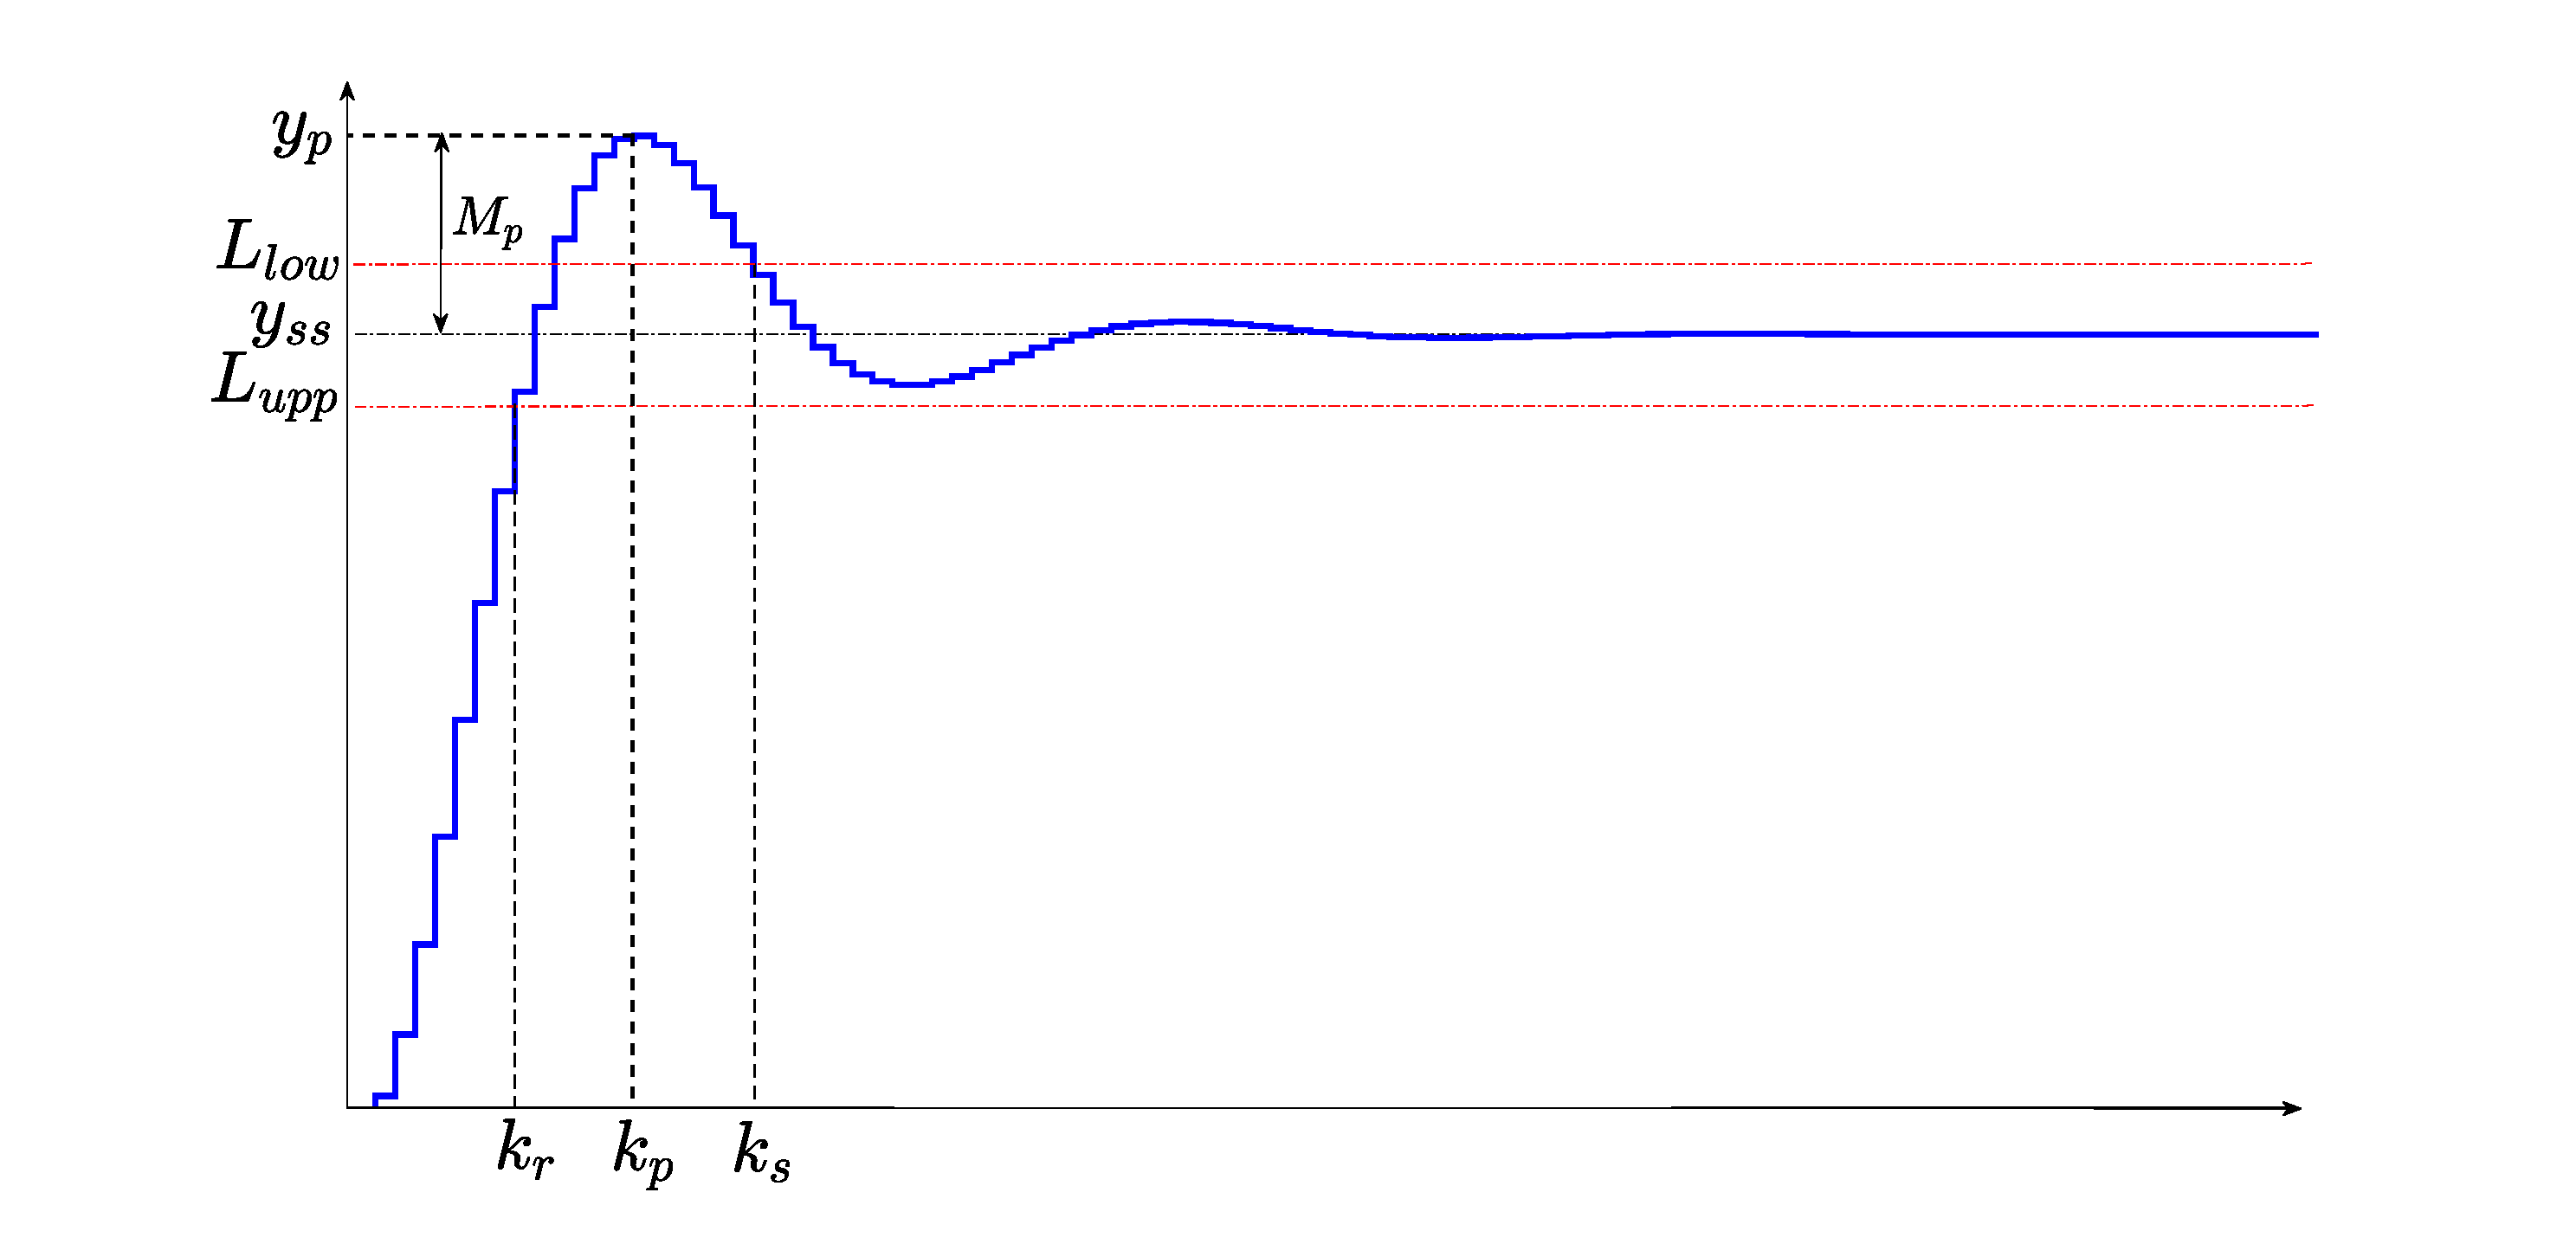
\includegraphics[trim={3.54cm 0cm 0cm 0cm}, clip, width=0.8\textwidth]{figures/output.eps}
			%}
	%}
	\caption{Step response of a discrete-time system.}
	\label{fig:output}
\end{figure}

\section{T�cnicas de Projeto de Controle para Sistemas Discretos}\label{sec:tpcsd}

Quando projetamos controladores para sistemas em tempo discreto, dispomos de muitas tecnicas para realizar o projeto. Muita das vezes, precisa-se fazer uma an�lise minunciosa da t�cnica a ser emprega, devido ao teor do projeto em quest�o. A seguir, mostraremos algumas das t�cnicas utilizadas atualmente e que mais tarde ser� feito uma compara��o das mesmas com a t�cnica que abordamos neste trabalho.

\subsection{Aloca��o de Polos}\label{subsec:ap}

Dado que o sistema em quest�o seja descrito como em (\ref{eq:ssed}), assumindo que tenha apenas um sinal de entrada, e o polin�mio caracter�stico da matrix $\mathbf{A}$ seja $P(z)=z^n+p_\mathrm{1}z^{\mathrm{n-1}}+\dots + p_n$. 
Assumindo que o sistema em (\ref{eq:ssed}) � alcan��vel, pode-se transform�-lo na forma can�nica, mudando as vari�veis de estado pela transforma��o $z=T_\mathrm{s}\mathbf{x}$, e a equa��o de estado transformado �

\begin{equation}\label{eq:ssed2}
z(k+1)=\hat{\mathbf{A}}z(k)+\hat{\mathbf{B}}\mathbf{u}(k)
\end{equation}

Com o sistema sendo alcan��vel, existe uma realimenta��o linear que fornece um sistema em malha fechada com polin�mio caracter�stico $P(z)$. A realimenta��o � dada por $\mathbf{u}[k]=-\mathrm{K}\mathbf{x}[k]$, com

\begin{equation}\label{eq:ctrlD}
\begin{aligned}
\mathbf{K}=&~(p_\mathrm{1}-a_\mathrm{1}~p_\mathrm{2}-a_\mathrm{2}~\dots~p_n-a_n)\hat{\mathbf{W}}_c \mathbf{W}_c^{-1} \\
          =&~(0~\dots~0~1)\mathbf{W}_c^{-1}P(\mathbf{A}) \\
\end{aligned},
\end{equation}

\noindent onde $\hat{\mathbf{W}}_c$ e $\mathbf{W}_c$ s�o as matrizes de alcan�abilidade de (\ref{eq:ssed2}) e (\ref{eq:ssed}), respectivamente.

\begin{equation}\label{eq:reachM1}
\hat{\mathbf{W}}^{-1}_c=\begin{bmatrix}
1 & a_\mathrm{1} & \dots & a_{n-1} \\
0 & 1 & \dots & a_{n-2} \\
\vdots & \vdots & \ddots & \vdots \\
0 & 0 & \dots & 1 
\end{bmatrix}
\end{equation}

\begin{equation}\label{eq:reachM2}
\mathbf{W}_c=(\mathbf{B}~\mathbf{A}\mathbf{B}\dots \mathbf{A}^{n-1}\mathbf{B})
\end{equation}




\subsection{Regulador Quadr�tico Linear}\label{subsec:rql}

O regulador quadr�tico linear LQR da teoria de controle �timo pode ser usado para resolver uma fam�lia de problemas de projeto do regulador em que o estado � acess�vel e a regula��o e o esfor�o do atuador s�o medidos por um desvio m�dio-quadrado. Uma formula��o estoc�stica do problema LQR � conveniente para n�s; uma formula��o mais usual � como um problema de controle �timo. O sistema � descrito por

\begin{equation*}
\dot{\mathbf{x}}=\mathbf{A}\mathbf{x}+\mathbf{B}\mathbf{u}+\mathbf{w},
\end{equation*}

\noindent onde $w$ � um ru�do branco de m�dia zero, isto �, $w$ tem matriz de densidade espectral de pot�ncia $S_\mathrm{w} (w) = I$ para todos $w$. O estado $\mathbf{x}$ est� dispon�vel para o controlador, ent�o $\mathbf{y} = \mathbf{x}$ nesse \textit{framework}.

A fun��o de custo do LQR � a soma do estado ponderado do quadrado m�dio do estado estacion�rio x, e o sinal do atuador ponderado do quadrado m�dio do estado estacion�rio u:

\begin{equation}
J_\mathrm{lqr} = \lim_{t\to \infty} \mathbf{E}(\mathbf{x}(t)^TQ\mathbf{x}(t)+\mathbf{u}(t)^TR\mathbf{u}(t)),
\end{equation}

\noindent onde Q e R s�o matrizes positivas de peso semidefinido; a
O primeiro termo penaliza os desvios de x de zero, e o segundo termo representa o custo de usar o sinal do atuador. Podemos expressar esse custo em nossa estrutura, formando o sinal de sa�da regulado $ \begin{bmatrix}
R^{\frac{1}{2}}u \\
Q^{\frac{1}{2}}x 
\end{bmatrix}  $, portanto, $J_\mathrm{lqr} = \lim_{t\to \infty} \mathbf{E}z(t)^Tz(t),$ o desvio quadr�tico m�dio de z. 

\subsection{S�ntese Indutiva Guidada por Contra Exemplos - CEGIS}\label{subsec:cegis}

\section{Implementa��o de Controladores Digitais}\label{subsec:icd}

\subsection{Efeitos de Palavra Finita}\label{subsec:fwl}



SMT (\textit{Satisfiability Modulo Theories}) verifica a satisfatibilidade de f�rmulas de primeira ordem a partir de uma ou mais teorias de fundamenta��o, que s�o compostas por um conjunto de senten�as. De modo formal, $\sigma$ -- \textit{theory} � uma cole��o de senten�as sobre a assinatura $\sigma$. Dada uma teoria $T$, diz-se que $\varphi$ � um m�dulo satisfat�vel de $T$ se $T \subset {\phi}$. Em outra defini��o, pode-se dizer que uma teoria $T$ � definida como uma classe de estruturas e $\varphi$ � um m�dulo satisfat�vel se existe uma estrutura $M$ em $T$ que satisfaz $\varphi$ (\textit{i.e.}, $M \models \varphi$)~\cite{Moura:2009}.

Solucionadores SMT como o Z3~\cite{Moura:2008} e Boolector~\cite{Brummayer:2009} suportam diferentes tipos de teorias, de modo que o seu desempenho pode variar conforme a sua implementa��o.

\begin{table}[htb]
	\renewcommand{\arraystretch}{1.0}
	\caption{Exemplos de teorias suportadas.}
	\label{table:smt}
	\centering
	\begin{tabular}{c|c}
		\hline \bfseries Teoria & \bfseries Exemplo\\
		\hline Igualdade & $x_1 = x_2 \wedge \neg (x_2 = x_3) \Rightarrow \neg (x_1 = x_3)$\\
		\hline Aritm�tica Linear & $(7y_1 + y_2 \geq 5) \vee (y_2 + y_3 \leq 2)$\\
		\hline Vetores de $bit$ & $(b \gg i) \& 1 = 1$\\
		\hline Arranjos & $store(a, j, 5) \Rightarrow a[j] = 5$\\
		\hline Teorias Combinadas & $(j \leq k \wedge a[j] = 2) \Rightarrow a[i] < 3$\\
		\hline
	\end{tabular}
\end{table}

A Tabela~\ref{table:smt} mostra algumas das teorias suportadas pelos solucionadores SMT utilizados neste trabalho. A teoria de igualdade permite verifica��es de igualdade e desigualdade entre predicados utilizando os operadores ($=$) ($\leq$) ($<$). A teoria da aritm�tica linear � respons�vel apenas pelas fun��es aritm�ticas (adi��o, subtra��o, multiplica��o e divis�o) entre vari�veis e constantes num�ricas. A teoria de vetores de $bit$ permite opera��es $bit$ a $bit$ considerando diferentes arquiteturas (\textit{e.g.}, $32$ e $64$ $bits$), nela est�o presentes os operadores: e ($\&$), ou ($\mid$), ou-exclusivo ($\bigoplus$), complemento ($\sim$), deslocamento para a direita ($\gg$) e deslocamento para a esquerda ($\ll$). Al�m disso, a teoria de arranjos permite a manipula��o de operadores como $select$ e $store$.

Em contraste com as f�rmulas geradas na satisfa��o booleana, que s�o apenas compostas por vari�veis booleanas, as quais podem assumir valores verdadeiro e falso e conectivos l�gicos, as f�rmulas de primeira ordem s�o formadas por conectivos l�gicos, vari�veis, quantificadores, fun��es e s�mbolos de predicado~\cite{Moura:2009}. De modo geral, as teorias do m�dulo da satisfatibilidade tem sido aplicadas em diversos cen�rios~\cite{Moura:2018}, apresentando resultados mais promissores (se comparados � satisfa��o booleana), incluindo o suporte a diferentes teorias de decis�o~\cite{Moura:2008, Moura:2009}.

\subsection{\textit{Efficient SMT-based Context-Bounded Model Checker}}\label{sec:esbmc}

O ESBMC � um verificador de modelos limitado ao contexto baseados nas teorias de m�dulo da satisfiabilidade (SMT), o qual � usado para verificar programas ANSI-C~\cite{Cordeiro:2012,DBLP:conf/tacas/MorseRCN014}. O ESBMC pode verificar tanto programas sequenciais quanto concorrentes e verifica propriedades relacionadas a estouro aritm�tico, divis�o por zero, acesso ilegal a posi��es em mem�ria, seguran�a de ponteiros, bloqueios fatais e corrida de dados. Esse processo � totalmente autom�tico e n�o requer intera��o de usu�rio para anotar programas com pr�- e/ou p�s-condi��es.

No ESBMC, o programa a ser verificado � modelado como um sistema de transi��o de estados $M = (S, R, s_0)$, 
que � extra�do de um gr�fico de fluxo de controle (GFC). $S$ representa o conjunto de estados, $R \subseteq S \times S$ representa o conjunto de transi��es ({\it i.e.}, pares de estados que especificam como o sistema pode navegar de um estado para outro) e $s_0 \subseteq S$ representa o conjunto de estadaos iniciais. Um estado $s \in S$ consiste de um valor do contador de programa $pc$ e os valores de todas as vari�veis do programa. Um estado inicial $s_0$ atribui a localiza��o inicial do programa do GFC para o $pc$. Cada transi��o $\gamma = (s_i, s_{i+1}) \in R$ entre dois estados $s_i$ and $s_{i+1}$ � identificada como uma f�rmula l�gica $\gamma (s_i,s_{i+1})$ que captura as restri��es nos valores do contador de programa e das vari�veis do programa correspondentes.

Dado um sistema de transi��o $M$, uma propriedade de seguran�a $\phi$, um limite de contexto $C$ e um limite $k$, o ESBMC constr�i uma �rvore de alcan�abilidade (AA) que representa o desdobramento do programa para $C$, $k$ e $\phi$. Ele ent�o deriva uma condi��o de verifica��o (CV)$\psi^{\pi}_k$, para cada intercala��o (ou caminho de computa��o) dada $\pi = \{v_1,...,v_k\}$, que � dada pela seguinte f�rmula l�gica:

\begin{equation}
\label{eq:bounded-model-checking}
    \psi^{\pi}_{k} =
    \overbrace{I(s_{0}) \wedge \bigvee_{i=0}^{k} \bigwedge_{j=0}^{i-1} \gamma(s_j,s_{j+1})}^{\textrm{restri��es}}
    \wedge \overbrace{\neg \phi(s_i)}^{\textrm{propriedade}}
\end{equation}

Aqui, $I$ caracteriza o conjunto de estados iniciais $M$ e $\gamma(s_j,s_{j+1})$ � a rela��o de $M$ entre passos de tempo $j$ e $j+1$. Consequentemente, $I(s_0) \wedge \bigvee_{j=0}^{i-1} \gamma (s_j,s_{j+1})$ representa a executa��o de $M$ de largura $i$ e $\psi^{\pi}_{k}$ pode ser satisfat�vel se e somente se para algum $i \leq k$ existe um estado alcan��vel ao longo de $\pi$ em um passo de tempo $i$ no qual $\phi$ � violada. $\psi^{\pi}_{k}$ � uma f�rmula livre de quantificadores em um subconjunto de l�gica de primeira ordem decid�vel, o qual sua satisfiabilidade � verificada por um solucionador SMT. Se $\psi^{\pi}_{k}$ � satisfat�vel, ent�o $\phi$ � violada ao longo de $\pi$ e o solucionador SMT fornece uma atribui��o satisfat�ria, da qual pode-se extrair valores para vari�veis do programa e construir um contraexemplo. Um contraexemplo para uma propriedade $\phi$ � uma sequ�ncia de estados $s_0,s_1,...,s_k$ com $s_0 \in S_0$, $s_k \in S$, e $\gamma (s_i, s_{i+1})$ para $0 \leq i < k$. Se $\psi^{\pi}_{k}$ n�o � satisfat�vel, pode-se concluir que nenhum estado de erro � alcan��vel em $k$ passos ou menos ao longo de $\pi$. Finalmente, pode-se definir $\psi_{k} = \bigwedge_{\pi} \psi_{k}^{\pi}$ e us�-la para verificar todos os caminhos.

No entanto, o ESBMC combina verifica��o de modelos simb�lica com a explora��o expl�cita do espa�o de estados; em particular, ele explicitamente explora todas as poss�veis intercala��es (at� o limite de contexto dado) enquanto ele trata cada intercala��o em si simbolicamente. O ESBMC implementa diferentes varia��es dessa abordagem, que diferem no modo que elas s�o exploradas na AA. A varia��o mais eficaz simplesmente percore a AA em profundidade e chama o procedimento BMC sequencial para cada intercala��o quando ela atinge um nodo folha da AA. Ele p�ra ou quando encontra erro ou sistematicamente explorou todas as poss�veis intercala��es da AA.

O modelo de mem�ria do ESBMC usa an�lise est�tica de ponteiros, preenchimentos em estruturas, com o objetivo de alinhar todos os campos aos limites de palavra, for�amento de regras de alinhamento de acesso de mem�ria e aloca��o de vetores de bytes, quando o tipo de aloca��o de mem�ria n�o � claro, para que a f�rmula SMT n�o seja t�o extensa e suscet�vel a erros.

O ESBMC tamb�m implementa a prova por indu��o~\cite{MorseCNF13,Gadelha:2017} para verificar propriedades em programas, \textit{i.e.}, utilizar uma abordagem iterativa de aprofundamento para checar se uma propriedade de seguran�a $\phi$ � satisfeita em cada passo $k$. O ESBMC usa um algoritmo \textit{k-induction}, que consiste de tr�s casos diferentes: caso base, condi��o adiante e passo indutivo. No caso base tenta-se encontrar um contraexemplo em at� $k$ desdobramentos de la�o; na condi��o adiante verifica-se se os la�os foram completamente desdobrados e que $\phi$ � v�lida em todos os estados alcan��veis dentro de $k$ passos; no passo indutivo assegura-se que sempre que $\phi$ � v�lida para $k$ desdobramentos, ela tamb�m � v�lida ap�s o pr�ximo desdobramento do sistema.

Uma outra aplica��o do ESBMC � a verifica��o de programas concorrentes para a plataforma CUDA~\cite{PereiraAMSCCSF16,Pereira:2016}. Utilizando um modelo operacional, \textit{i.e.}, uma representa��o abstrata das bibliotecas CUDA padr�es que aproxima de forma conservadora as suas sem�nticas, o ESBMC � capaz de verificar propriedades de seguran�a em programas CUDA. Al�m disso, o ESBMC implementa a redu��o parcial de ordem e a an�lise de duas \textit{threads} para minimizar a explora��o de espa�o de estados.

\section{Localiza��o de Falhas e Verifica��o de Modelos}\label{sec:fault-localization-and-model-checking}

\subsection{Uso de Contraexemplos para Localizar Falhas}\label{sec:using-counterexamples}

Em verifica��o de modelos, a atividade mais essencial, em rela��o � localiza��o de falhas, � a de gera��o de um contraexemplo, o qual � produzido quando um programa n�o satisfaz uma dada especifica��o. Um contraexemplo n�o prov� unicamente informa��es sobre a rela��o causa-efeito de uma dada viola��o, mas ele tamb�m pode auxiliar na localiza��o de falhas, como Clarke {\it et al.}~\cite{Clarke:2003,Clarke:1995} citam. Mas, visto que uma grande massa de informa��o � obtida em um contraexemplo, as linhas de fato defeituosas n�o s�o facilmente identificadas.

Alguns m�todos foram propostos, com o objetivo de localizar poss�veis causas de falha, usando contraexemplos. Ball {\it et al.}~\cite{Ball:2003} propuseram uma abordagem que tenta isolar poss�veis causas de contraexemplos, gerados pelo verificador de modelos SLAM~\cite{Ball:2001}. A ideia � que potenciais linhas defeituosas podem ser isoladas atrav�s de uma compara��o entre as transi��es obtidas em contraexemplos e execu��es bem-sucedidas, visto que transi��es n�o presentes em rastreamentos bem-sucedidos s�o potenciais causas de erros. Groce {\it et al.}~\cite{Groce:2003} afirmam que se um contraexemplo existe, um caminho similar mas n�o-defeituoso tamb�m existe e pode ser obtido usando t�cnicas de BMC. Elementos de programa relacionados a uma dada viola��o s�o sugeridos pelas diferen�as entre tal contraexemplo e um caminho bem-sucedido. Tal abordagem � implementada no verificador de modelos {\it Java PathFinder}~\cite{JPF} e tamb�m pode porver caminhos de execu��o que levam a estados err�neos, com rela��o a programasa concorrentes ({\it e.g.}, corrida de dados). O conceito chave da abordagem descrita por Groce {\it et al.}~\cite{Groce:2006} � similar ao anterior e usa alinhamento de restri��es para associar estados, em um contraexemplo, com os estados correspondentes em uma execu��o n�o-defeituosa, os quais s�o gerados por um solucionador de restri��es. Os estados mencionados s�o estados abstratos sobre predicados, os quais representam estados concretos em uma execu��o. Usando propriedades de m�tricas de dist�ncia, restri��es podem ser aplicadas para representar execu��es do programa, e restri��es sem correspondentes que representam estados concretos possivelmente levam a falhas. E ainda, se uma propriedade de m�tricas de dist�nica n�o � satisfeita, um contraexemplo � gerado pelo verificador de modelos~\cite{Groce:2006}.

\subsection{Localiza��o de Falhas em Programas Sequenciais}\label{sec:sequential-fault-localization}

Griesmayer {\it et al.}~\cite{Griesmayer:2007} propuseram um m�todo baseado em t�cnicas de BMC que pode diretamente identificar potenciais falhas em programas. Em particular, o m�todo usa vari�veis num�ricas adicionais, {\it e.g.} \texttt{diag}, para apontar linhas defeituosas em um dado programa.

Cada linha do programa, representando uma declara��o \texttt{S}, � transformada em uma vers�o l�gica de tal declara��o. Logo, o valor atribu�do a \texttt{S} � ou n�o-deterministicamente escolhido pelo verificador de modelos (se o valor de \texttt{diag} for o mesmo que o representado pela linha relacionada � declara��o \texttt{S}) ou o especificado originalmente. Os valores de \texttt{diag} obtidos pelo verificador de modelos representam linhas do programa e est�o estritamente ligados � falha obtida, visto que, corrigindo essa linha no programa original, a falha em quest�o pode ser evitada. No caso de m�ltiplos valores de \texttt{diag}, corrigindo tais linhas levam a uma execu��o bem sucedida do programa. Com o intuito de encontrar o conjunto inteiro de linhas que causam o comportamento defeituoso no programa, uma nova especifica��o no comando de verifica��o\footnote{\texttt{assume(diag != a)}} pode ser adicionada ao c�digo-fonte, o qual ent�o � executado novamente pelo verificador de modelos. Esse processo � executado repetidamente at� que n�o sejam obtidos novos valores para \texttt{diag}, {\it i.e.}, a execu��o n�o falha~\cite{Griesmayer:2007_2}.

Para ilustrar o funcionamento do m�todo em quest�o, toma-se como exemplo um controlador digital baseado na f�rmula da fun��o hor�ria do movimento retil�neo uniformemente variado (MRUV)~\cite{Ohanian:2006} (veja Equa��o~\ref{equation:space-equation}). A equa��o do controlador � definida na Equa��o~\ref{equation:controller-equation} (os valores foram atribu�dos arbritariamente).

\begin{gather}
  s(t) = at^2/2+v_0t+s_0 \label{equation:space-equation}
\end{gather}

\begin{gather}
  c(t) = t^2-3t+2 \label{equation:controller-equation}
\end{gather}

Um modelo na linguagem C do controlador � modelado como na Figura~\ref{figure:sequential-code}.

\begin{figure}[ht]
\centering
\begin{minipage}{0.65\textwidth}
\begin{lstlisting}
#include <stdio.h>
#include <assert.h>

const int A = 1;
const int B = -2;
const int C = 2;

int controller(int input) {
  int output = A * input * input + B * input + C;
  return output;
}

int main() {
  assert(controller(0) == 2 && controller(1) == 0 && controller(2) == 0 && controller(3) == 2);
  return 0;
}
\end{lstlisting}
\end{minipage}
\caption{C�digo sequencial de um controlador qualquer.}
\label{figure:sequential-code}
\end{figure}

Pode-se observar que o modelo n�o est� em conformidade com a equa��o dada, no caso o termo $B$ est� com o valor $-2$ ao inv�s de $-3$. Dessa forma, espera-se que a assertiva falhe ao executar o programa em um verificador de modelos, como pode ser observado no trecho da Figura~\ref{figure:counterexample-model} (o contraexemplo completo est� dispon�vel no Ap�ndice~\ref{appendix:counterexample-1}).

\begin{figure}[ht]
\centering
\begin{minipage}{0.65\textwidth}
\begin{lstlisting}
...
Violated property:
  file model.c line 14 function main
  assertion 
  FALSE

VERIFICATION FAILED
\end{lstlisting}
\end{minipage}
\caption{Trecho do contraexemplo para o modelo.}
\label{figure:counterexample-model}
\end{figure}

Usando o ESMBC como verificador de modelos, o c�digo instrumentado n�o-determin�stico obtido � como na Figura~\ref{figure:griesmayer-method-applied-code}.

\begin{figure}[ht]
\centering
\begin{minipage}{0.65\textwidth}
\begin{lstlisting}
#include <stdio.h>
#include <assert.h>
const int A = 1;
const int B = -2;
const int C = 2;
int nondet(int i) {
  int ret;
  __ESBMC_assume(ret != i);
  return ret;
}
int controller(int input) {
  int diag = nondet(0);
  int ta = (diag == 1 ? nondet(A) : A) * input * input;
  int tb = (diag == 2 ? nondet(B) : B) * input;
  int tc = (diag == 3 ? nondet(C) : C);
  int output = ta + tb + tc;
  return output;
}
int main() {
  __ESBMC_assume(controller(0) == 2 && controller(1) == 0 && controller(2) == 0 && controller(3) == 2);
  assert(0);
  return 0;
}
\end{lstlisting}
\end{minipage}
\caption{C�digo sequencial instrumentado com o m�todo descrito aplicado.}
\label{figure:griesmayer-method-applied-code}
\end{figure}

Ao executar o c�digo da Figura~\ref{figure:griesmayer-method-applied-code} no ESBMC sucessivamente, \textit{i.e.}, at� que n�o sejam encontrados novos valores para $diag$, obt�m-se os valores presentes na Figura~\ref{figure:faulty-lines-griesmayer} (o contraexemplo completo est� dispon�vel no Ap�ndice~\ref{appendix:counterexample-2}).

\begin{figure}[ht]
\centering
\begin{minipage}{0.65\textwidth}
\begin{lstlisting}
griesmayer::controller::1::diag=-2012462479 (-2012462479)
griesmayer::controller::1::diag=2 (2)
griesmayer::controller::1::diag=2 (2)
griesmayer::controller::1::diag=2 (2)
\end{lstlisting}
\end{minipage}
\caption{Linhas defeituosas obtidas pela execu��o do c�digo~\ref{figure:griesmayer-method-applied-code}.}
\label{figure:faulty-lines-griesmayer}
\end{figure}

Segundo o contraexemplo obtido com o ESBMC, pode-se observar que o valor de $diag$ � $2$ em tr�s casos e um inteiro negativo em um caso. Logo, o problema est� no c�lculo do segundo termo, como esperado. O contraexemplo completo mostra que o valor para corrigir tal falha � $-3$. Assim, pode-se corrigir a falha apontada e reexecutar o c�digo no verificador de modelos.

\begin{figure}[ht]
\centering
\begin{minipage}{0.65\textwidth}
\begin{lstlisting}
#include <stdio.h>
#include <assert.h>
const int A = 1;
const int B = -3;
const int C = 2;
int controller(int input) {
  int output = A * input * input + B * input + C;
  return output;
}
int main() {
  assert(controller(0) == 2 && controller(1) == 0 && controller(2) == 0 && controller(3) == 2);
  return 0;
}
\end{lstlisting}
\end{minipage}
\caption{C�digo sequencial corrigido.}
\label{figure:corrected-sequential-code}
\end{figure}

Ap�s a corre��o do problema apontado, executa-se o c�digo corrigido~\ref{figure:corrected-sequential-code} no ESBMC e obt�m-se as linhas presentes na Figura~\ref{figure:correct-faulty-lines-griesmayer} (o contraexemplo completo est� dispon�vel no Ap�ndice~\ref{appendix:counterexample-3}). Em controladores digitais, � importante que os modelos sejam precisamente especificados para evitar falhas durante o funcionamento em ambiente real, visto que podem levar ao mal-funcionamento do equipamento e at� danos, aumentando o custo do mesmo.

\begin{figure}[ht]
\centering
\begin{minipage}{0.65\textwidth}
\begin{lstlisting}
griesmayer::controller::1::diag=-934770697 (-934770697)
griesmayer::controller::1::diag=-1 (-1)
griesmayer::controller::1::diag=-1 (-1)
griesmayer::controller::1::diag=-1 (-1)
\end{lstlisting}
\end{minipage}
\caption{Linhas defeituosas obtidas pela execu��o do c�digo~\ref{figure:corrected-sequential-code}.}
\label{figure:correct-faulty-lines-griesmayer}
\end{figure}

Dessa forma, foi poss�vel observar o m�todo proposto por Griesmayer {\it et al.}~\cite{Griesmayer:2007} aplicado em um programa sequencial.

Este m�todo foi escolhido para ser utilizado neste trabalho, pois al�m de ser simples a sua implementa��o, ele aponta n�o s� linhas que cont�m defeitos, como tamb�m poss�veis valores que levam a uma execu��o bem-sucedida do programa original.

\section{Resumo}\label{sec:chap-2-summary}

Neste cap�tulo, foram introduzidos os conceitos b�sicos para o entendimento desta disserta��o, relacionadas � verifica��o de modelos. Mais especificamente, explicou-se o conceito de verifica��o de modelos limitada usando teorias de m�dulo da satisfiabilidade (SMT) com o verificador de modelos ESBMC ({\it Efficient SMT-based Context-Bounded Model Checker}), que verifica propriedades de programas sequenciais e concorrentes. Tamb�m foram mostradas discuss�es sobre o uso de contraexemplos para auxiliar no processo de localiza��o de falhas. Por fim, foi apresentado um m�todo para localizar falhas em programas sequenciais, usando n�o-determinismo para instrumentar atribui��es, de forma que o verificador de modelos escolhe o valor para cada vari�vel do programa para que propriedade (em forma de assertiva) presente no c�digo seja satisfeita. Como resultado, o cont�udo deste cap�tulo fornece todo o embasamento necess�rio para compreens�o do trabalho desenvolvido, que ser� descrito nas se��es subsequentes.

\chapter{Trabalhos Relacionados}\label{chap_related_work}

Neste cap�tulo, ser�o descritos oito trabalhos relacionados que direta ou indiretamente abordam localiza��o de falhas em programas concorrentes. Apesar de existirem outros estudos relacionados ao tema, foram selecionados apenas os que se assemelham a este trabalho.

Cada trabalho relacionado ser� descrito de acordo com suas caracter�sticas mais relevantes. Ao final de cada subse��o ser�o destacados os melhores aspectos e os pontos fracos de cada um. Por fim, ser� feito um paralelo das caracter�sticas que s�o importantes para os objetivos propostos neste trabalho, que servir� como base de compara��o.

\section{\textit{Formal Non-Fragile Stability Verification of Digital Control Systems with Uncertainty}}\label{sec:related-work-1}

Bessa {\it et al.}~\cite{bessa2017formal} apresentam uma metodologia de verifica��o para determinar formalmente a estabilidade incerta de sistemas lineares em controladores digitais com considera��es sobre os aspectos de implementa��o. Especificamente, esta estrat�gia � combinada com o DSVerifier, que � uma ferramenta de verifica��o que utiliza a verifica��o de modelo limitado com base nas teorias de m�dulo de confiabilidade (SMT) para verificar a estabilidade dos sistemas de controle digital considerando incerteza. O DSVerifier determina a estabilidade do sistema de controle, considerando a planta, juntamente com os efeitos do comprimento da palavra finita (FWL) na implementa��o do controlador digital. Em seguinda, verifica-se a estabilidade robusta ``n�o fr�gil'' de um determinado sistema em malha fechada. A metodologia proposta e a respectiva ferramenta (DSVerifier) s�o avaliadas considerando exemplos de controle n�o fr�geis encontrados na literatura.

O trabalho mostra que a t�cnica � capaz de prever problemas de fragilidade em controladores robustos quando consideramos a estabilidades de sistemas de controle digital, visto que leva em considera��o os efeito FWL. No entanto, este trabalho se prende a apenas verificar a estabilidade, sendo que aspectos de desempenho s�o deixados de lado, visto que as propriedades de desempenho s�o super importantes quando se projeta controladores, al�m de j� considerarem a estabilidade.

\section{\textit{Formal Analysis of Robustness at Model and Code Level }}\label{sec:related-work-2}

Wang {\it et al.}~\cite{WangGRJF16} apresentam uma abordagem de verifica��o da robustez de sistemas de controle, a nivel de c�digo e modelagem, onde se baseia em um c�lculo invariante na din�mica discreta do sistema. Usando solucionadores de programa��o semi-definida (SDP), uma fun��o baseada em Lyapunov � sintetizada, capturando as margens do vetor do sistema linear em malha fechada considerado. Essa invariante num�rica expressa sobre as vari�veis de estado do sistema � compat�vel com a an�lise de c�digo e permite sua valida��o no artefato de c�digo. Esta an�lise autom�tica amplia as t�cnicas de verifica��o focadas na implementa��o do controlador, abordando a valida��o da robustez no modelo e no n�vel de c�digo. Ele foi implementado em uma ferramenta que analisa sistemas SISO discretos e gera super-aproxima��es de margens de fase e ganho.

Os autores apresentam uma abordagem eficaz para verificar robustez dos controladores digitais a nivel de c�digo e modelagem. Novamente, esse trabalho emprega a verifica��o usando uma abordagem a nivel de c�digo, por�m n�o considera aspectos de desempenho do controlador, apesar de considerar aspectos relativos a efeitos causados pela aritm�tica de ponto fixo.

\section{\textit{Temporal Logic Control of Discrete-Time Piecewise Affine Systems}}\label{sec:related-work-3}

Yordanov {\it et al.}~\cite{yordanov2012temporal} apresentam uma estrutura computacional para s�ntese autom�tica de uma estrat�gia de controle de realimenta��o para um sistema de tempo discreto (mais precisamente sistemas PWA) a partir de uma especifica��o dada como uma l�gica linear temporal (LTL) sobre um conjunto arbitr�rio de predicados lineares nas vari�veis de estado do sistema. A abordagem consiste em definir parti��es apropriadas para seu estado e espa�os de entrada, e ent�o constr�i-se uma abstra��o finita do sistema na forma de um sistema de transi��o de controle. Depois disso, aproveitando ideias e t�cnicas de verifica��o de modelos LTL e jogos de Rabin, desenvelvoram um algoritmo para gerar uma estrat�gia de controle para a abstra��o finita.

A abordagem apresentada para a constru��o da abstra��o garante que uma estrat�gia de controle gerada para o sistema de controle finito pode ser facilmente transformada em uma estrat�gia de controle para o sistema PWA inicial. Embora comprovadamente correta, a solu��o geral � conservadora e computacionalmente cara. Apesar de esta abordagem conseguir sintetizar controladores, deixa de considerar alguns aspectos bem relevantes em projetos de controladores digitais, como aspectos de desempenho e efeitos da fragilidade de controladores quando implementados em microprocessadores.

\section{\textit{Formal Methods for Adaptive Control of Dynamical Systems}}\label{sec:related-work-4}

Sadraddini and Belta~\cite{sadraddini2017formal} desenvolveram um m�todo para controlar sistemas de tempo discreto com par�metros constantes mas inicialmente desconhecidos a partir de especifica��es de l�gica temporal linear (LTL).Os autores usam as no��es de sistemas de transi��o param�tricos e adaptativos (n�o-determin�sticos) e ferramentas de m�todos formais para computar estrat�gias de controle adaptativo para sistemas finitos. 

Apesar de n�o utilizar os m�todos tradicionais de controle adaptativo, usando uma abordagem correta por constru��o a qual n�o requer um modelo de refer�ncia e pode lidar com uma gama muito maior de sistemas e especifica��es, n�o leva em considera��o aspectos relativos a depensempenho de sistemas considerando a resposta ao degrau, bem como deixa de lado aspectos enfrentados com a implementa��o, como os efeitos de fwl. Como a maioria das outras aplica��es de m�todos formais, os resultados sofrem pela alta complexidade computacional. Como discutido no artigo, o n�mero de estados no sistema de transi��o adaptativa (ATS) pode ser muito grande. Al�m disso, a constru��o de quocientes finitos para sistemas infinitos � computacionalmente dif�cil.

\section{\textit{Correct-by-construction Adaptive Cruise Control: Two Approaches}}\label{sec:related-work-5}

Nilsosn {\it et al.}~\cite{nilsson2016correct} descrevem duas abordagens para sintetizar controladores correto por constru��o em istemas de controle de cruzeiro adaptativo. Ambas as abordagens baseiam-se na computa��o em pontos fixos no dom�nio do controlador, a partir da qual a especi?ca��o em l�gica linear temporal (LTL) pode ser aplicada. Uma calcula tais pontos fixos diretamente no espa�o de estados cont�nuo, a outra em uma abstra��o de estados finitos da din�mica n�o-linear.

De acordo com os resultados experimentais, este trabalho se mostra eficaz para sistemas de controle de cruzeiro adaptativo. Por�m, leva em considera��o a s�ntese de controladores est�veis considerando a propriedade de \textit{safety}, mas n'ao aborda quest�es de projeto de controladores referentes a desempenho a resposta ao degrau.

\section{\textit{Formal Specification and Analysis Approaches for Spacecraft Attitude Control Requirements}}\label{sec:related-work-6}

Gross {\it et al.}~\cite{gross2017formal} propuseram uma abordagem para formalizar requisitos comuns de sistema de controle de atitude de naves espaciais, como limites do atuador, erro de indica��o, alcan�abilidade, desvio, tempo de assentamento, tempo de subida e sobressinal. Os autores utlizaram m�todos formais, mais especificamente verifica��o de modelos e teste de hip�tese para verificar requisitos de desempenho de sistemas de controle de atitude de naves espaciais. O trabalho em quest�o avalia esses sistemas e verifica se obedecem a esses requisitos no dom�nio do tempo cont�nuo. Embora a inten��o inicial de formalizar os requisitos fosse conduzir an�lises formais de m�todos para determinar se o projeto de controle de atitude de naves espaciais atendia aos requisitos do sistema, as equa��es de movimentos n�o-lineares se mostraram muito complexas para os solucionadores e apenas alguns requisitos puderam ser analisados.

Um ponto positivo desse trabalho foi que consideraram aspectos de desempenho na verifica��o de controladores. Apesar disso, os autores n�o trabalharam com sistemas em tempo discreto, n�o levando em considera��o aspectos de implementa��o, como os efeitos fwl.

\section{\textit{Formal Synthesis of Analytic Controllers for Sampled-Data Systems via Genetic Programming.}}\label{sec:related-work-7}

Park {\it et al.}~\cite{Park:2014} apresentam um m�todo de localiza��o de falhas din�mico para localizar as ra�zes da causa de defeitos de concorr�ncia e a implementa��o de um prot�tipo da t�cnica, chamado \textsc{Falcon}. Usando detec��o din�mica de padr�es e localiza��o de falhas estat�stica, o \textsc{Falcon} � capaz de mostrar a exist�ncia de defeitos em programas concorrentes, tanto de atomicidade quanto viola��o de ordem, auxiliando desenvolvedores a corrigir falhas em c�digos. A t�cnica utiliza dados providos por casos de teste para o programa em verifica��o e tenta encontrar padr�es pr�-estabelecidos de acesso � mem�ria compartilhada. Tais padr�es s�o organizados estatisticamente de forma a priorizar quais as poss�veis falhas existentes no programa.

De acordo com o estudo emp�rico realizado pelos autores, a t�cnica aparentou ser eficaz para tratar viola��es de atomicidade e ordem em programa concorrentes, mostrando-se eficiente em termos de espa�o e tempo utilizado. No entanto, essa abordagem foi desenvolvida apenas para lidar com programas Java, depende de casos de teste para a procura por padr�es defeituosos e, no trabalho em quest�o, os autores apenas avaliaram a ferramenta com uma entrada de teste e m�ltiplas execu��es do programa.

\section{\textit{Cause Clue Clauses: Error Localization using Maximum Satisfiability}}\label{sec:related-work-8}

Jose {\it et al.}~\cite{Jose:2011} discutem sobre um algoritmo para localiza��o de causas de erro, considerando uma redu��o para o {\it problema da satisfiabilidade m�xima} (MAX-SAT), que aponta o n�mero m�ximo de cl�usulas de uma f�rmula booleana que uma atribui��o pode satisfazer simultaneamente. A ideia chave � combinar uma f�rmula de rastreamento booleana e uma f�rmula n�o-satisfat�vel, ambas em rela��o ao desdobramento do programa e uma execu��o do programa malsucedida, e usar MAX-SAT para encontrar o conjunto m�ximo de cl�usulas que podem ser satisfeitas ao mesmo tempo nessa f�rmula. O complemento desse conjunto devolvido pelo solucionador MAX-SAT cont�m os locais do programa que levam ao erro, logo, corrigindo esses locais, � poss�vel conseguir uma execu��o sem falhas do programa para o caso de teste dado. Vale ressaltar que o uso de MAX-SAT tamb�m foi abordado por Trindade {\it et al.}~\cite{Trindade:2016} no ESBMC para avaliar o problema de particionamento de hardware-software.

O algoritmo apresentado � capaz de localizar linhas defeituosas e os autores tamb�m realizaram experimentos para sugerir reparos de atribui��es aritm�ticas e troca de operadores de compara��o no c�digo original. Apesar dessa abordagem ser �til para localizar linhas defeituosas, ela ainda depende de uma execu��o malsucedida, e funciona apenas para para programas ANSI-C padr�o.

\section{\textit{Automated Formal Synthesis of Digital Controllers for State-Space Physical Plants}}

Hong {\it et al.}~\cite{abate2017automated} prop�em uma abordagem s�lida e automatizada para sintetizar controladores digitais com realimenta��o seguros para plantas f�sicas representadas como modelos lineares invariantes no tempo. Os autores utilizaram s�ntese indutiva guiada por contra-exemplo (CEGIS) o qual possui duas fases: s�ntese de um controlador de realimenta��o est�tico que estabiliza o sistema, mas que pode n�o ser seguro para todas as condi��es iniciais. A seguran�a � ent�o verificada via verifica��o de modelos limitada (BMC, do ingl�s \textit{bounded model checking}) ou acelera��o abstrata; se a etapa de verifica��o falhar, um contra-exemplo � fornecido ao mecanismo de s�ntese e o processo itera at� que um controlador seguro seja obtido.

O trabalho em quest�o apresenta excelentes resultados, por�m ainda deixa de considerar aspectos desempenho de projeto de controladores, considerando somente a estabilidade dos mesmos. Um bom aspecto � que a metodologia considera fragilidade na implementa��o dos controladores digitais.

\section{\textit{Metallaxis-FL: Mutation-Based Fault Localization}}

Papadakis {\it et al.}~\cite{Papadakis:2015} apresentam uma abordagem de localiza��o de falhas baseadas em an�lise de muta��o, chamada \textit{Metallaxis}. A abordagem consiste em usar mutantes e associ�-los com potenciais locais defeituosos do programa, e quando mutantes s�o mortos (principalment por casos de testes que falham), tais s�o essencialmente bons indicadores sobre os locais defeituosos de um programa.  Ainda mais, a abordagem apresentada usa em seu favor um n�mero alto de casos de teste para ordenar instru��es mutadas, com rela��o � sua pontua��o de suspeita, o qual leva a falhas no programa. De acordo com dados experimentais, \textit{Metallaxis} � substancialmente mais efetivo que abordagens baseadas em instru��es, at� quando t�cnicas de redu��o de custo de muta��o (\textit{e.g.}, amostragem de muta��o) s�o usada. \textit{Metallaxis} localiza falhas efetivamente e, visto que ele funciona sobre uma su�te de teste, ele s� pode ser usado durante o teste para localizar potenciais falhas.

A abordagem se mostra superior a abordagens baseadas em instru��es; no entanto, ela ainda deende de uma extensa su�te de teste e s� foi avaliada em software ANSI-C procedural/sequencial.

\section{Compara��o entre os Trabalhos}

Os trabalhos relacionados tratam ou de localiza��o de falhas em programas ou em verifica��o de programas concorrentes. Foi poss�vel observar que o problema de localiza��o de falhas � pertinente, visto que este processo toma muito tempo dos desenvolvedores no ciclo de desenvolvimento de software. O tratamento de programas concorrentes tamb�m foi observado como um problema complexo de ser tratado devido ao grande n�mero de possibilidades nas tentativas de simular um comportamento defeituoso. Tendo esses pontos em mente, as principais diferen�as entre a abordagem proposta nesse trabalho para as aqui discutidas podem ser listadas: o m�todo proposto requer apenas o c�digo-fonte do programa, em contraste com outros m�todos, onde mais dados s�o necess�rios, como uma execu��o malsucedida; o m�todo proposto funciona para programas concorrentes em C, amplamente usados em sistemas embarcados; e, finalmente, � poss�vel apontar linhas defeituosas facilmente, enquanto que outras abordagens verificam a seguran�a de um programa. A Tabela~\ref{table:related-work-comparison} mostra um quadro comparativo entre o m�todo proposto nesta disserta��o e os trabalhos relacionados selecionados.

\begin{table}[ht]
    \renewcommand{\arraystretch}{1.0}
    \caption{Compara��o dos trabalhos relacionados}
    \label{table:related-work-comparison}
    \centering
    \begin{tabular}{c|c|c|c|c}
        \hline \shortstack{\bfseries Trabalhos} & \bfseries Localiza & \bfseries Aplic�vel em & \bfseries Verifica & \bfseries Necessita\\
\bfseries relacionados & \bfseries falhas & \bfseries programas & \bfseries c�digo & \bfseries de casos\\
\bfseries & & \bfseries concorrentes & \bfseries C & \bfseries de teste\\
        \hline Jones {\it et al.} (2009) & X & & X & X\\
        \hline Cleve {\it et al.} (2005) & X & & X & X\\
        \hline Birch {\it et al.} (2015) & X & & X & X\\
        \hline Tomasco {\it et al.} (2015) & & X & X &\\
        \hline Cordeiro {\it et al.} (2011) & & X & X &\\
        \hline Griesmayer {\it et al.} (2007) & X & & X &\\
        \hline Park {\it et al.} (2014) & X & X & &\\
        \hline Jose {\it et al.} (2011) & X & & X &\\
        \hline Hong {\it et al.} (2015) & X & & X & X\\
        \hline Papadakis {\it et al.} (2015) & X & & X & X\\
        \hline M�todo proposto & X & X & X &\\
	\end{tabular}
\end{table}

Atrav�s da Tabela~\ref{table:related-work-comparison} pode-se observar que existem outros trabalhos que s�o capazes de localizar falhas em programas concorrentes. No entanto, nenhum deles � capaz de atingir ambos objetivos em programas escritos na linguagem C e, ainda mais, sem o aux�lio de casos de teste previamente escritos, diferentemente do m�todo proposto.

\section{Resumo}\label{chap-3-summary}

Neste cap�tulo foram apresentados diversos trabalhos relacionados a algum dos seguintes problemas: localiza��o de falhas, suporte a programas concorrentes, verifica��o de c�digo escrito na linguagem C e/ou depend�ncia de casos de testes externos. Ap�s a apresenta��o de cada t�cnica, assim como uma breve discuss�o sobre as vantagens e desvantagens de cada uma delas, foi feita uma compara��o com o m�todo proposto neste trabalho. Foi poss�vel observar que o m�todo proposto aborda os tr�s primeiros itens sem a necessidade de casos de testes externos, o que o diferencia dos demais trabalhos. O pr�ximo cap�tulo apresenta a metodologia proposta para localizar falhas em programas concorrentes utilizando t�cnicas de sequencializa��o e BMC.
\chapter{A Metodologia Proposta}\label{chap_methodology}

Neste cap�tulo, o m�todo proposto para localizar falhas em programas concorrentes em C ser� completamente descrito. Primeiramente, um exemplo de motiva��o ser� apresentado para descrever a abordagem. Os passos anteriores � localiza��o de falhas, onde t�cnicas de BMC s�o aplicadas, s�o mostrados a seguir. Tamb�m s�o descritas as regras de transforma��o para sequencializar um programa concorrente. Finalmente, uma explica��o � dada sobre o processo de localiza��o de falhas no programa concorrente transformado.

\section{Vis�o Geral do M�todo}
\label{sec:method-overview}

Aqui, o m�todo proposto � descrito brevemente, como mostrado na Figura~\ref{figure:methodology}, e uma explica��o mais detalhada � exposta nas se��es seguitnes. Dado um programa concorrente $P$, primeiramente checa-se se ele apresenta uma execu��o mal-sucedida com rela��o a uma determinada intercala��o. Para realizar tal tarefa, $P$ � executado em um verificador de modelos duas vezes: a primeira execu��o verifica se existe algum bloqueio fatal e a segunda � respons�vel por outros tipos de viola��o, tais como erros de aquisi��o de sem�foro, divis�o por zero, seguran�a de ponteiros, estouro aritm�tico e viola��o de limites de vetores. N�o � poss�vel verific�-lo apenas uma vez porque os verificadores de modelos separam essas verifica��es, \textit{i.e.}, � necess�rio adicionar uma op��o de linha de comando para habilitar a detec��o de bloqueios fatais e ignorar viola��es devido a assertivas. Caso um contraexemplo possa ser obtido nesse passo, � poss�vel prosseguir com o m�todo. Ent�o, o pr�ximo passo define as regras de transforma��o, que s�o as instru��es sequenciais que substituir�o as originais concorrentes, e um arcabou�o sequencial, o qual tem como objetivo simular a execu��o concorrente da intercala��o mal-sucedida. O terceiro passo consiste em usar o m�todo proposto por Griesmayer~\cite{Griesmayer:2007} para instrumentar atribui��es e express�es, de forma a apontar locais e instru��es defeituosas do programa. Tal programa instrumentado pode ent�o ser executado, usando um verificador de modelos, e � poss�vel coletar as linhas defeituosas, at� que a verifica��o associada n�o produza diferentes elementos. Essa itera��o � descrita na Figura~\ref{figure:methodology} por meio dos passos $3$, $4$, j� que o m�todo busca novos contraexemplos, com o intuito de encontrar novas linhas defeituosas. Finalmente, as linhas defeituosas s�o obtidas, assim como atribui��es necess�rias para produzir uma execu��o bem-sucedida de $P$.

\begin{figure}[ht]
  \centering
  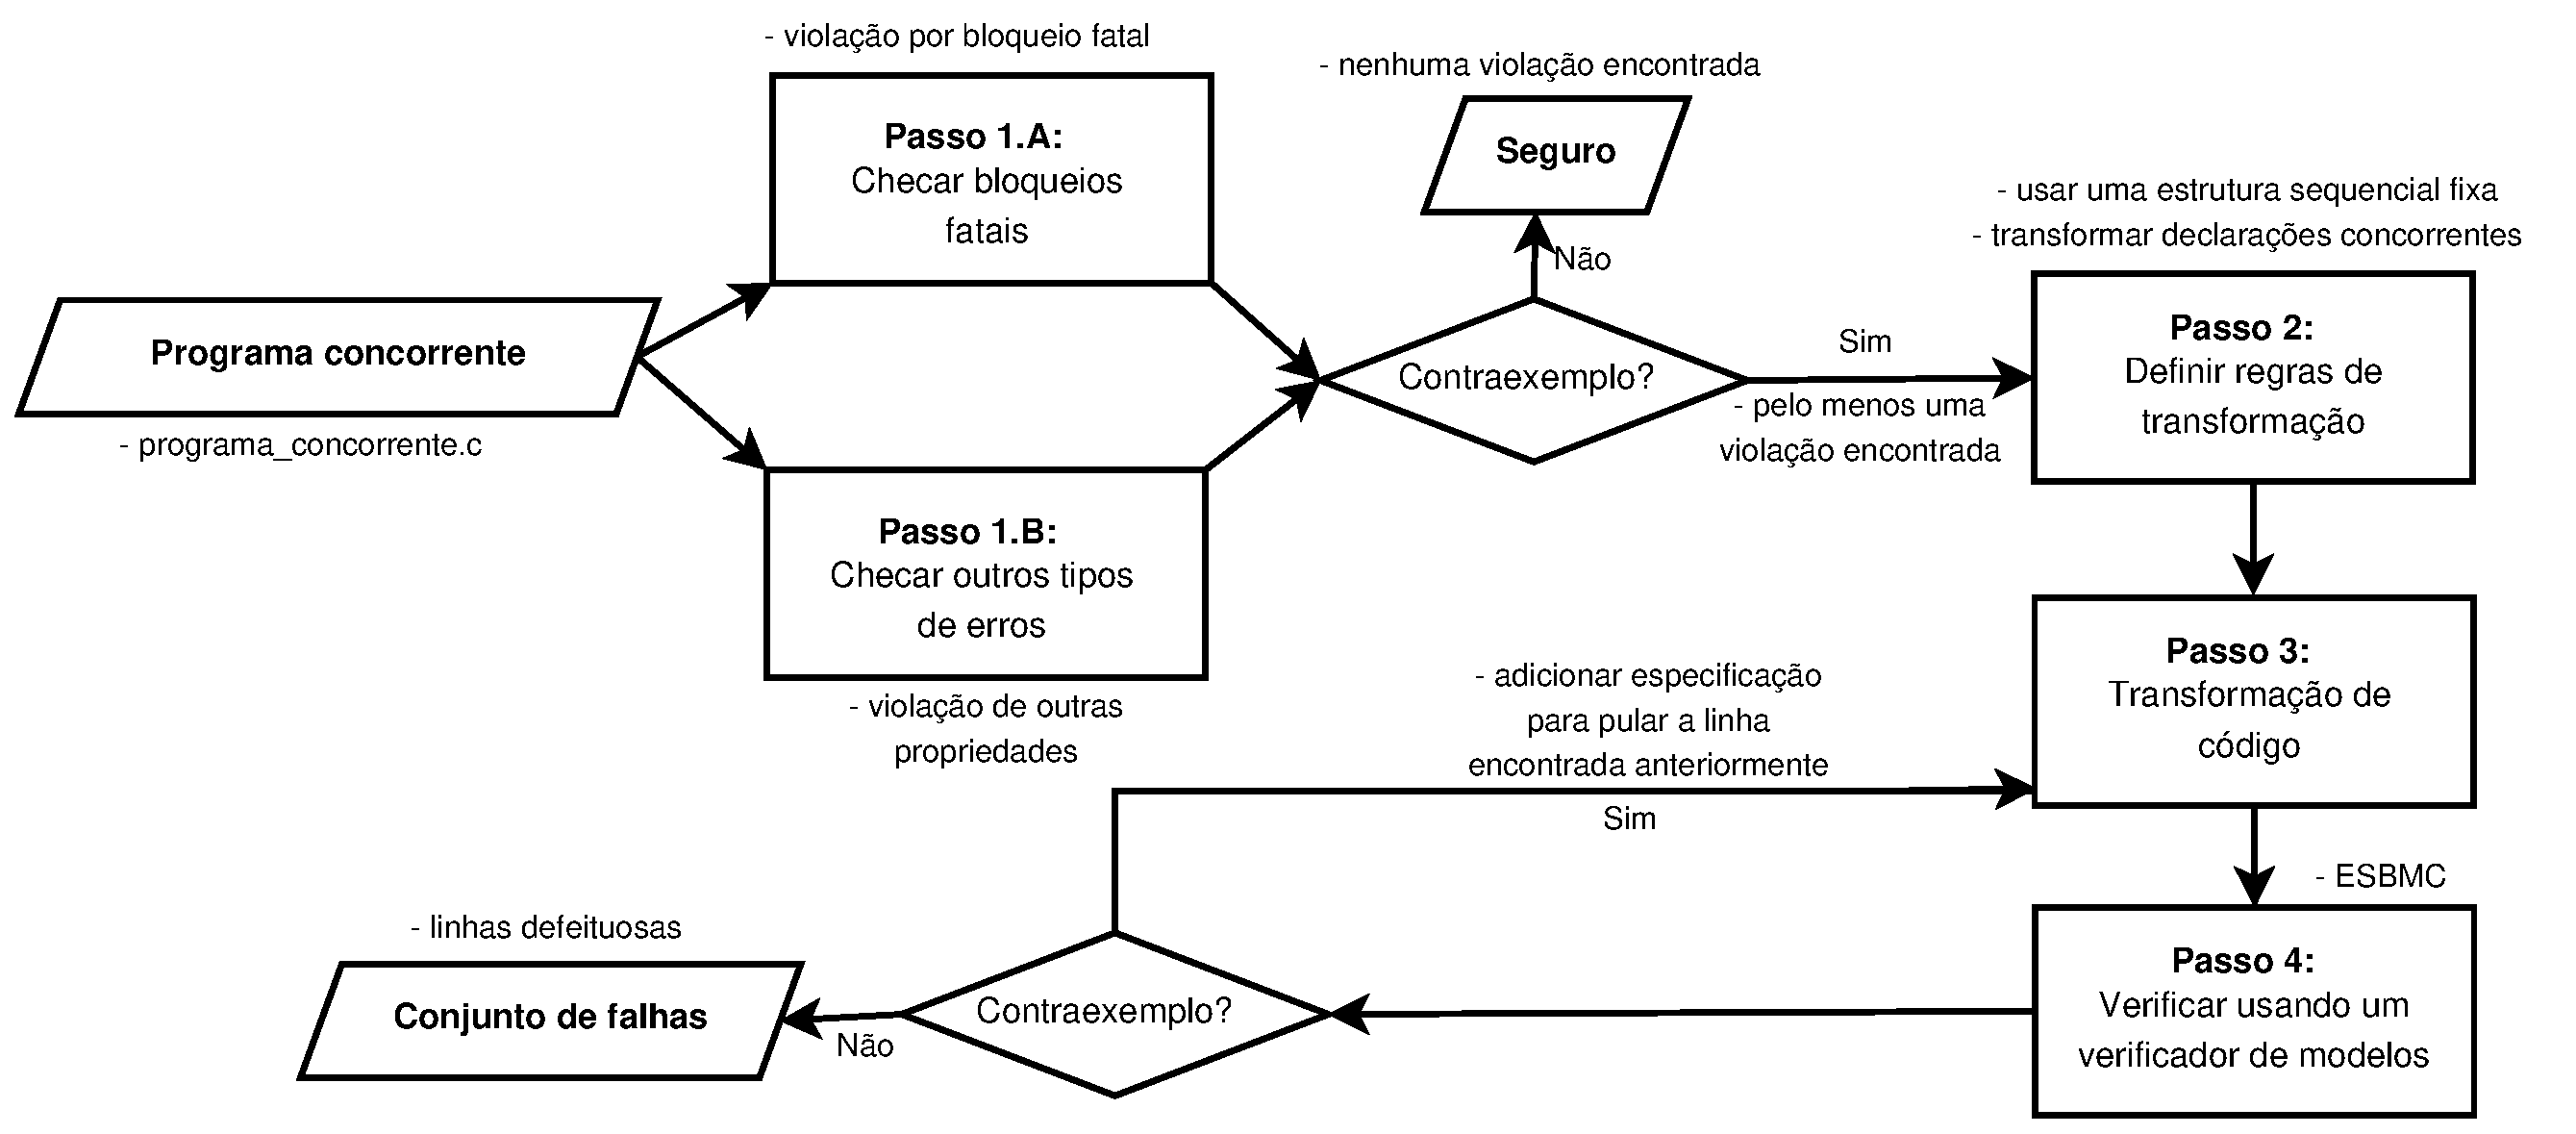
\includegraphics[scale=0.35]{figures/methodology}
  \caption{Metodologia proposta.}
  \label{figure:methodology}
\end{figure}

\section{Exemplos Motivacionais}\label{sec:running-example}

Dois programas concorrentes simples s�o utilizados para ilustrar a abordagem proposta. O primeiro (ver Figura~\ref{figure:example-1}) tem duas vari�veis compartilhadas, os sem�foros \texttt{mutex} e \texttt{lock}, usados para sincronizar as {\it threads} \texttt{A} e \texttt{B}. A fun��o \texttt{main} inicializa cada contador da sua respectiva {\it thread} e come�a a executar duas {\it threads}, executando as fun��es \texttt{threadA} e \texttt{threadB}, respectivamente. Cada fun��o de {\it thread} adquire o sem�foro \texttt{mutex}, incrementa o seu respectivo contador (\texttt{A\_count} ou \texttt{B\_count}), verifica se � poss��vel adquirir o sem�foro \texttt{lock} (caso seu contador seja igual a um), libera o sem�foro \texttt{mutex}, tenta adquirir o sem�foro \texttt{mutex} logo em seguida, decrementa o seu contador, verifica se � poss��vel liberar o sem�foro \texttt{lock} (caso seu contador seja zero), e finalmente libera o sem�foro \texttt{mutex}. Visto que n�o h� assertivas, n�o se deve obter outros tipos de viola��es, a n�o ser erros de concorr�ncia. Pode-se notar que o controle de acesso ao sem�foro \texttt{lock} � feito de forma local. Assumindo que trocas de contexto podem ocorrer em qualquer linha do programa, � prov�vel que uma execu��o espec�fica leve a um erro de bloqueio fatal.
%
\begin{figure}[htb]
\centering
\begin{minipage}{0.65\textwidth}
\begin{lstlisting}
void *threadA(void *arg) {
	pthread_mutex_lock(&mutex);
	A_count++;
	if (A_count == 1) pthread_mutex_lock(&lock);
	pthread_mutex_unlock(&mutex);
	pthread_mutex_lock(&mutex);
	A_count--;
	if (A_count == 0) pthread_mutex_unlock(&lock);
	pthread_mutex_unlock(&mutex);
}
void *threadB(void *arg) {
	pthread_mutex_lock(&mutex);
	B_count++;
	if (B_count == 1) pthread_mutex_lock(&lock);
	pthread_mutex_unlock(&mutex);
	pthread_mutex_lock(&mutex);
	B_count--;
	if (B_count == 0) pthread_mutex_unlock(&lock);
	pthread_mutex_unlock(&mutex);
}
int main() {
	pthread_t A, B;
	A_count = 0; B_count = 0;
	pthread_create(&A, NULL, threadA, NULL);
	pthread_create(&B, NULL, threadB, NULL);
	pthread_join(A, NULL);
	pthread_join(B, NULL);
	return EXIT_SUCCESS;
}
\end{lstlisting}
\end{minipage}
\caption{Primeiro exemplo motivacional.}
\label{figure:example-1}
\end{figure}

Para transformar um c�digo concorrente para sequencial, deve-se, em linhas gerais, transformar declara��es de programa concorrentes para vers�es sequenciais que tenham o mesmo comportamento e adicionar uma estrutura fixa para que o novo programa sequencial execute da mesma forma que o original, processo que ser� descrito nas pr�ximas se��es. Aplicando tais passos no c�digo da Figura~\ref{figure:example-1}, tem-se como resultado o c�digo mostrado nas Figuras~\ref{figure:hawk-applied-example-1-p1} e~\ref{figure:hawk-applied-example-1-p2}. Com o m�todo aplicado no c�digo concorrente, o restante do processo de localiza��o de falhas depende apenas do verificador de modelos em uso, que retornar� informa��es �teis relacionadas �s falhas existentes no programa (o contraexemplo simplificado para esse c�digo est� dispon�vel no Ap�ndice~\ref{appendix:counterexample-4}).

\begin{figure}[h!]
\centering
\begin{minipage}{0.65\textwidth}
\begin{lstlisting}
... int non_det(), diag;
int A_count, B_count;
h_mutex mutex, lock;
void A_1(void *arg) {
	int t;
	h_cs cs;
	h_lock(&mutex, &cs, 1, 9);
	t = A_count;
	A_count = (diag == 10 ? non_det() : t + 1);
	if ((diag == 11 ? non_det() : A_count) == 1)
		h_lock(&lock, &cs, 1, 11);
	h_unlock(&mutex, &cs, 1, 12);
}
void A_2(void *arg) {
	int t;
	h_cs cs;
	h_lock(&mutex, &cs, 1, 13);
	t = A_count;
	A_count = (diag == 14 ? non_det() : t - 1);
	if ((diag == 15 ? non_det() : A_count) == 0)
		h_unlock(&lock, &cs, 1, 15);
	h_unlock(&mutex, &cs, 1, 16);
}
void B_1(void *arg) {
	int t;
	h_cs cs;
	h_lock(&mutex, &cs, 2, 20);
	t = B_count;
	B_count = (diag == 21 ? non_det() : t + 1);
	if ((diag == 22 ? non_det() : B_count) == 1)
		h_lock(&lock, &cs, 2, 22);
}
void B_2(void *arg) { ... } ...
\end{lstlisting}
\end{minipage}
\caption{M�todo aplicado ao exemplo da Figura~\ref{figure:example-1} (parte $1$).}
\label{figure:hawk-applied-example-1-p1}
\end{figure}

\begin{figure}[h!]
\centering
\begin{minipage}{0.65\textwidth}
\begin{lstlisting}
... #define NCS 4
int cs[] = {11, 21, 31, 22};
int main() {
	int i;
	diag = non_det();
	for (i = 0; i < NCS; i++) {
		switch (cs[i]) {
			case 1: {
				case 11: {
					A_count = 0; B_count = 0;
					if (cs[i] == 11) break;
				}
			} break;
			case 2: {
				case 21: {
					A_1(NULL);
					if (cs[i] == 21) break;
				}
				case 22: {
					A_2(NULL);
					if (cs[i] == 22) break;
				}
			} break;
			case 3: {
				case 31: {
					B_1(NULL);
					if (cs[i] == 31) break;
				}
			} break;
		}
	}
	assert(0);
}
\end{lstlisting}
\end{minipage}
\caption{M�todo aplicado ao exemplo da Figura~\ref{figure:example-1} (parte $2$).}
\label{figure:hawk-applied-example-1-p2}
\end{figure}

O segundo (ver Figura~\ref{figure:example-2}) cont�m duas vari�veis globais, \texttt{x} e \texttt{y}, utilizadas por cada uma das \textit{threads} existentes no programa. A primeira \textit{thread} incrementa o valor de \texttt{x} e a segunda decrementa o valor de \texttt{y}. Ambas \textit{threads} s�o executadas e finalmente � verificada uma propriedade, \textit{i.e.}, ambas as vari�veis devem ter um valor positivo.

\begin{figure}[htb]
\centering
\begin{minipage}{0.65\textwidth}
\begin{lstlisting}
... int x = 0, y = 0;
void* sum_x(void* args) {
    x++;
    return NULL;
}
void* sum_y(void* args) {
    y--;
    return NULL;
}
int main(void) {
    pthread_t t1, t2;
    pthread_create(&t1, NULL, sum_x, NULL);
    pthread_create(&t2, NULL, sum_y, NULL);
    pthread_join(t1, NULL);
    pthread_join(t2, NULL);
    assert(x > 0 && y > 0);
    return 0;
}
\end{lstlisting}
\end{minipage}
\caption{Segundo exemplo motivacional.}
\label{figure:example-2}
\end{figure}

Utilizando os mesmos passos ilustrados no exemplo anterior, obt�m-se o c�digo da Figura~\ref{figure:example-2}, tem-se como resultado o c�digo mostrado na Figura~\ref{figure:hawk-applied-example-2}. De forma similar, o verificador de modelos retornar� informa��es �teis relacionadas �s falhas existentes no programa (o contraexemplo simplificado para esse c�digo est� dispon�vel no Ap�ndice~\ref{appendix:counterexample-5}), assim como valores poss�veis para reproduzir uma execu��o bem-sucedida do mesmo. A seguir, ser� explicada a metodologia por completo, resumida na Figura~\ref{figure:methodology}.

\begin{figure}[h!]
\centering
\begin{minipage}{0.65\textwidth}
\begin{lstlisting}
...
int main(void) {
    int cs[] = { 11, 21, 31, 12 };
    int ncs  = 4;
    int diag = nondet_int();
    int x, y;
    for (int i = 0; i < ncs; i++) {
        switch (cs[i]) {
            case 1: {
                case 11: {
                    x = 0;
                    y = 0;
                    if (cs[i] == 11) break;
                }
                case 12: {
                    if (cs[i] == 12) break;
                }
            } break;
            case 2: {
                case 21: {
                    int temp = x + 1;
                    x = (diag == 7 ? nondet_int() : temp);
                    if (cs[i] == 21) break;
                }
            } break;
            case 3: {
                case 31: {
                    int temp = y - 1;
                    y = (diag == 12 ? nondet_int() : temp);
                    if (cs[i] == 31) break;
                }
            } break;
        }
    }
    __ESBMC_assume(x > 0 && y > 0);
    assert(0);
    return 0;
}
\end{lstlisting}
\end{minipage}
\caption{M�todo aplicado ao exemplo da Figura~\ref{figure:example-2}.}
\label{figure:hawk-applied-example-2}
\end{figure}

\section{Uso de BMC para Auxiliar na Localiza��o de Falhas}\label{sec:bmc-usage}

\subsection{Assegurando a Exist�ncia de Falhas em Programas Concorrentes}\label{sec:unsafety}

De forma que seja poss�vel aplicar a metodolgia proposta, � necess�rio assegurar a exist�ncia de falhas do programa concorrente $P$ sob verifica��o (\textbf{Passo 1.A} e \textbf{Passo 1.B} da Figura~\ref{figure:methodology}). Para alcan�ar tal objetivo, � necess�rio pelo menos uma propriedade violada (erro de bloqueio fatal, assertiva, aquisi��o de sem�foro, divis�o por zero, seguran�a de ponteiros, estouro aritm�tico, e/ou viola��o de limites de vetores) e o seu respectivo contraexemplo (veja Se��o~\ref{sec:esbmc} para mais detalhes), informa��o que pode ser obtida por meio da verifica��o de $P$ em um verificador de modelos duas vezes. Se um contraexemplo para $P$ n�o puder ser encontrado, ou o limite $k$ � aumentado (limitado aos recursos de m�quina dispon�veis) ou afirma-se que $P$ � seguro ($P$ n�o cont�m falhas) at� a profundidade $k$.

\subsection{Extra��o de Informa��es das Trocas de Contexto de Contraexemplos}\label{sec:context-switch}

Com posse de um contraexemplo $C_{ex}$ para $P$, � necess�rio extrair as informa��es de trocas de contexto para posteriormente aplic�-las com o objetivo de encontrar um programa sequencial $P_{seq}$ que reproduza o mesmo comportamento defeituoso que $P$ tem (\textbf{Passo 2} da Figura~\ref{figure:methodology}).

Para que seja poss�vel obter tal informa��o, seja $C_{ex}$ composto por um conjunto de estados $s_0,s_1,...,s_k$. Cada estado $s_i$ cont�m a linha $l_{s_i}$ e a {\it thread} $T_{s_i}$ a qual tal estado pertence. Anotando a tupla $(T_{s_i},l_{s_i})$ onde $T_{s_i} \neq T_{s_{i+1}}$ resulta nas trocas de contexto que ocorrem em $P$ para o dado comportamento defeituoso. Por exemplo, em rela��o ao programa da Figura~\ref{figure:example-1}, a informa��o de troca de contexto obtida do seu respectivo contraexemplo � $CS = [(0,27),(1,5),(2,14),(1,6)]$, onde a {\it thread} $0$ representa a fun��o \texttt{main}, a {\it thread} $1$ representa a {\it thread} $A$ e a {\it thread} $2$ representa a {\it thread} $B$.

\section{Sequencializa��o de Programas Concorrentes}\label{sec:sequentialization}

\subsection{Modelagem das Primitivas de Sincroniza��o da Biblioteca \textit{Phtread}}\label{sec:pthread}

Levando em considera��o a sequentializa��o, � necess�rio modelar as declara��es de programa originalmente concorrentes para obter uma vers�o sequencial de tais declara��es, mantendo suas respectivas funcionalidades (\textbf{Passo 2} da Figura~\ref{figure:methodology}).

Primeiramente, uma estrutura do tipo \texttt{struct} foi desenvolvida para representar trocas de contexto. S�o armazenadas as vari�veis \texttt{thread\_ID}, um identificador para a {\it thread} onde a troca de contexto ocorreu, e \texttt{program\_line}, um identificador para a linha do programa onde a troca de contexto ocorreu. Essa estrutura � chamada \texttt{h\_cs} e � definida como na Figura~\ref{figure:hawk-cs}.
%
\begin{figure}[htb]
\centering
\begin{minipage}{0.4\textwidth}
\begin{lstlisting}
typedef struct h_context_switch {
	int thread_ID;
	int program_line;
} h_cs;
\end{lstlisting}
\end{minipage}
\caption{Estrutura que representa uma troca de contexto.}
\label{figure:hawk-cs}
\end{figure}

Ent�o, desenvolveu-se uma estrutura do tipo \texttt{struct} para representar uma vari�vel do tipo \texttt{pthread\_mutex\_t}. S�o armazenadas as vari�veis \texttt{status}, um identificador para dizer se tal sem�foro est� adquirido ou n�o, e \texttt{last\_cs}, identificando as informa��es do programa relacionadas � aquisi��o ou libera��o de tal sem�foro. Essa estrutura � chamada \texttt{h\_mutex} e � definida como na Figura~\ref{figure:hawk-mutex}.
%
\begin{figure}[htb]
\centering
\begin{minipage}{0.3\textwidth}
\begin{lstlisting}
typedef struct h_mutex {
	int status;
	h_cs last_cs;
} h_mutex;
\end{lstlisting}
\end{minipage}
\caption{Estrutura que representa o tipo \texttt{pthread\_mutex\_t}.}
\label{figure:hawk-mutex}
\end{figure}

Implementa��es para a manipula��o de sem�foros, que s�o a aquisi��o de um sem�foro, \texttt{pthread\_mutex\_lock}, e a libera��o de um sem�foro, \texttt{pthread\_mutex\_unlock}. A fun��o que representa a aquisi��o de um sem�foro tem $4$ argumentos, que s�o \texttt{m} (o sem�foro que uma {\it thread} est� tentando adquirir), \texttt{cs} (uma vari�vel de troca de contexto), \texttt{id} (um identificador para a {\it thread} que chamou a fun��o de aquisi��o), e \texttt{line} (um identificador para a linha do programa de onde a fun��o foi chamada). A fun��o de libera��o tamb�m tem $4$ argumentos, que s�o \texttt{m} (o sem�foro que uma {\it thread} est� tentando liberar), \texttt{cs} (uma vari�vel de troca de contexto), \texttt{id} (um identificador para a {\it thread} que chamou a fun��o de libera��o), e \texttt{line} (um identificador para a linha do programa de onde a fun��o foi chamada). A fun��o de aquisi��o � chamada \texttt{h\_lock} e � definida como na Figura~\ref{figure:hawk-mutex-lock}. A fun��o de libera��o � chamada \texttt{h\_unlock} e � definida como na Figura~\ref{figure:hawk-mutex-unlock}.

Vari�veis condicionais s�o implementadas em {\it pthread} como na Figura~\ref{figure:pthread-conditionals}. De forma a simular o mesmo comportamento, a execu��o n�o precisa ser parada. Visto que se simula apenas um comportamento defeituoso, a condi��o necess�ria � assumida como j� satisfeita, ent�o basicamente muda-se a vari�vel do tipo \texttt{pthread\_cond\_t} para o tipo inteiro, a fun��o \texttt{pthread\_cond\_signal} atribui $0$ a tal variavel, e a fun��o \texttt{pthread\_cond\_signal} atribui $1$. Esse processo � descrito na Figura~\ref{figure:hawk-conditionals}, como uma modelagem do c�digo da Figura~\ref{figure:pthread-conditionals}.
%
\begin{figure}[htb]
\centering
\begin{minipage}{0.35\textwidth}
\begin{lstlisting}
pthread_cond_t c;
...
	pthread_cond_signal(&c, &m);
...
while (!condition) {
	pthread_cond_wait(&c, &m);
}
\end{lstlisting}
\end{minipage}
\caption{Uso de vari�veis condicionais padr�o.}
\label{figure:pthread-conditionals}
\end{figure}

\begin{figure}[ht]
\centering
\begin{minipage}{0.35\textwidth}
\begin{lstlisting}
int c;
...
	c = 0;
...
while (!condition) {
	c = 1;
	break;
}
\end{lstlisting}
\end{minipage}
\caption{Modelagem de condicionais no m�todo proposto.}
\label{figure:hawk-conditionals}
\end{figure}

%
\begin{figure}[htb]
\centering
\begin{minipage}{0.5\textwidth}
\begin{lstlisting}
void h_lock(h_mutex *m,
			h_cs *cs,
			int id,
			int line) {
	int status = m->status;
	if (status == 1) {
		__VERIFIER_error();
	} else {
		cs->thread_ID = id;
		cs->program_line = line;
		m->status = 1;
		m->last_cs.thread_ID = cs->thread_ID;
		m->last_cs.program_line = cs->program_line;
	}
}
\end{lstlisting}
\end{minipage}
\caption{Modelagem da fun��o \texttt{pthread\_mutex\_lock}.}
\label{figure:hawk-mutex-lock}
\end{figure}
%
\begin{figure}[htb]
\centering
\begin{minipage}{0.5\textwidth}
\begin{lstlisting}
void h_unlock(h_mutex *m,
			  h_cs *cs,
			  int id,
			  int line) {
	if (m->status == 1 &&
			m->last_cs.thread_ID == id) {
		cs->thread_ID = id;
		cs->program_line = line;
		m->status = 0;
		m->last_cs.thread_ID = cs->thread_ID;
		m->last_cs.program_line = cs->program_line;
	} else {
		__VERIFIER_error();
	}
}
\end{lstlisting}
\end{minipage}
\caption{Modelagem da fun��o \texttt{pthread\_mutex\_unlock}.}
\label{figure:hawk-mutex-unlock}
\end{figure}

A Tabela~\ref{table:rules} resume todas as regras desenvolvidas neste trabalho para transformar programas concorrentes em sequenciais. A coluna \textit{``\#''} representa os dois grupos de instru��es de programas, \textit{i.e.}, ($1$) normal e ($2$) concorrente, a coluna \textit{``Fragmento de c�digo''} mostra o c�digo a ser transformado, e as colunas \textit{``Sem bloqueio fatal''} and \textit{``Com bloqueio fatal''} dizem qual regra de transforma��o precisa ser executada, caso um programa apresente ou n�o um bloqueio fatal, respectivamente.

\begin{table}[htb!]
%\renewcommand{\arraystretch}{0.97}
\renewcommand\arraystretch{0.97}
\caption{Regras para transformar programas concorrentes}
\label{table:rules}
\centering\small
\begin{tabular}{c|c|c|c}
\hline \bfseries \# & \bfseries Fragmento de c�digo & \bfseries Sem bloqueio fatal & \bfseries Com bloqueio fatal\\
\hline \multirow{3}{*}{1}&Declara��o&Sem altera��es&Sem altera��es\\ &Express�o&Desdobramento&Desdobramento\\&Instru��o&Sem altera��es&Sem altera��es\\
\hline \multirow{11}{*}{2}&\texttt{pthread\_t}&$\epsilon$&$\epsilon$\\
&\texttt{pthread\_attr\_t}&$\epsilon$&$\epsilon$\\
&\texttt{pthread\_cond\_attr\_t}&$\epsilon$&$\epsilon$\\
&\texttt{pthread\_create}&$\epsilon$&$\epsilon$\\
&\texttt{pthread\_join}&$\epsilon$&$\epsilon$\\
&\texttt{pthread\_exit}&$\epsilon$&$\epsilon$\\
&\texttt{pthread\_mutex\_t}&$\epsilon$&Sem�foro � declarado\\
&\texttt{pthread\_mutex\_lock}&$\epsilon$&Aquisi��o � chamada usando a vari�vel\\
&\texttt{pthread\_mutex\_unlock}&$\epsilon$&Libera��o � chamada usando a vari�vel\\
&\texttt{pthread\_cond\_t}&$\epsilon$&Vari�vel condicional � declarada\\
&\texttt{pthread\_cond\_wait}&$\epsilon$&Parada � chamada usando a vari�vel\\
&\texttt{pthread\_cond\_signal}&$\epsilon$&Sinaliza��o � chamada usando a vari�vel\\
\hline
\end{tabular}
\end{table}

\subsection{Adi��o de uma Estrutura Fixa para Simula��o}\label{sec:framework}

Uma estrutura fixa prov� a mesma sequ�ncia de execu��o presente no programa original. Ela consiste basicamente em escrever cada c�digo de {\it thread} dentro de um bloco condicional \texttt{case}, e as suas respectivas sequ�ncias de execu��o s�o especificadas no vetor \texttt{cs}. Tal estrutura � usada como a estrutura base para novas vers�es sequenciais de programas concorrentes (\textbf{Passo 2} da Figura~\ref{figure:methodology}) e a Figura~\ref{figure:framework} mostra como � tal codifica��o.
%
\begin{figure}[htb]
\centering
\begin{minipage}{0.45\textwidth}
\begin{lstlisting}
#define NCS X
int cs[] = {...};
int main(int argc, char *argv[]) {
	int i;
	for(i = 0; i < NCS; i++) {
	  switch(cs[i]) {
	    case 1:
    	    case 11: { ... }
    	    ...
    	    case 20: { ... }
	    break;
	    case 2:
    	    case 21: { ... }
    	    ...
    	    case 30: { ... }
	    break;
	    case 3:
	        case 31: { ... }
    	    ...
    	    case 40: { ... }
    	break;
	    ...
	    default:
	    break;
	  }
	}
	return 1;
}
\end{lstlisting}
\end{minipage}
\caption{A estrutura padr�o para sequencializar programas concorrentes.}
\label{figure:framework}
\end{figure}

Como se pode notar, a estrutura fixa mencionada prov� novas posi��es fixas para cada parte do c�digo original e a Tabela~\ref{table:relation} mostra a rela��o entre as novas posi��es e o tipo de fragmento de c�digo, isto �, ela resume como o novo c�digo sequencial � estruturado. Em particular, elementos globais, vari�veis globais, declara��es de arquivos de bibliotecas e outros tipos de declara��es globais s�o posicionadas antes da fun��o \texttt{main} do c�digo sequencial. O corpo da sua fun��o \texttt{main}, do c�digo original, � posicionado entre a declara��o do \texttt{case 1} e seu respectivo comando \texttt{break}, o corpo da primeira {\it thread} � posicionado entre a declara��o do \texttt{case 2} e seu respectivo comando \texttt{break}, e assim por diante. Esse processo � repetido at� que n�o existam mais {\it threads} para serem inseridas na vers�o sequencial do c�digo. Adicionalmente, os argumentos passados para a fun��o \texttt{main} do programa original s�o todos passados para a fun��o \texttt{main} da vers�o sequencial. Em casos onde {\it threads} s�o parcialmente executadas, uma troca de contexto ocorre, outra {\it thread} � executada ou uma {\it thread} anterior continua a execu��o do ponto onde a mesma parou, os respectivos trechos de c�digo s�o inseridos em cada bloco \texttt{case} dentro do bloco maior $N^{th}$ \texttt{case} (o $N^{th}$ \texttt{case} representa a $N^{th}$ {\it thread}), de tal forma que a ordem de execu��o permance a mesma.
%
\begin{table}[htb]
	\renewcommand{\arraystretch}{1.0}
	\caption{Rela��o entre as posi��es no programa e o c�digo original}
	\label{table:relation}
	\centering
	\begin{tabular}{c|c}
		\hline \bfseries Tipo de fragmento de c�digo & \bfseries Posi��o no\\
		\bfseries no c�digo original & \bfseries novo c�digo sequencial\\
		\hline elementos globais & antes da linha $1$\\
		\hline corpo da fun��o principal & entre o ''case $1$'' e o ''break''\\
		\hline corpo da {\it thread} $n$ & entre o ''case $n + 1$'' e o ''break''\\
		\hline
	\end{tabular}
\end{table}

De forma a manter a mesma ordem de execu��o encontrada no programa original, o controle da ordem do \texttt{switch} � necess�rio. Uma ordem de trocas de contexto, obtida por meio de um contraexemplo do programa concorrente, pode ser copiada para o novo c�digo sequencial, controlando os blocos \texttt{case} e as declara��es condicionais\footnotemark dentro do bloco \texttt{switch}. Em linhas gerais, o processo de adi��o de controle de ordem de trocas de contexto para o novo programa sequencial pode ser dividido em dois passos. Com o intuito de mostrar uma situa��o simples de tal passo, assume-se que existem no m�ximo $10$ trocas de contexto em cada {\it thread} ($\forall N_{ti}, N_{ti} < 10$), um contraexemplo, dado pelo verificador de modelos, tem $N$ trocas de contexto, e dentre essas $N$ trocas de contexto, $N_{t0}$ ocorrem na fun��o \texttt{main} do programa, $N_{t1}$ ocorrem na {\it thread} $1$, $N_{t2}$ na {\it thread} $2$, e assim por diante, de forma que $(N_{t0} + ... + N_{tn} = N)$.

O primeiro passo � obter informa��es dos contraexemplos gerados pelo verificador de modelos, {\it i.e.}, o n�mero total de trocas de contexto no programa original e em cada {\it thread}, a ordem de todas as trocas de contexto por todo o programa e tamb�m em cada {\it thread} isolada, e a posi��o correspondente onde uma troca de contexto ocorreu. Com tais dados, � poss�vel adicionar declara��es condicionais\footnotemark[\value{footnote}] para manter a mesma ordem de execu��o do programa original, de forma que quando uma linha � executada, o c�digo sequencial executa o pr�ximo bloco \texttt{case}, o qual representa a pr�xima {\it thread} no programa original.

\footnotetext{\texttt{if (cs[i]) == Y) break;}, onde \texttt{Y} representa o n�mero da troca de contexto relacionada}

Pode-se notar que se existem la�os iterativos no programa original concorrente, para cada la�o, uma vari�vel global \texttt{loopcounter} � adicionada. Al�m disso, a declara��o para incrementar o valor da vari�vel \texttt{loopcounter} tamb�m � adicionado ao fim do bloco de cada la�o. Essa nova vari�vel global adicionada � usada como uma condi��o para controlar diretamente os comandos \texttt{break}, de forma que quando uma troca de contexto ocorre, dentro de um la�o, o valor atribu�do � vari�vel \texttt{loopcounter} tamb�m deve ser respectivamente usado no comando \texttt{break}, de forma a manter a sequ�ncia de execu��o original do programa.

O segundo passo consiste em modificador os valores relacionados ao vetor \texttt{cs}, de tal forma que a ordem de execu��o � mantida, no novo programa sequencial. Mudando as linhas $1$ e $2$, na Figura~\ref{figure:framework}, de acordo com o n�mero espec�fico de trocas de contexto existentes e as suas respectivas ordens de execu��o, � poss�vel garantir a ordem de execu��o original, visto que o bloco \texttt{switch} (linha $6$) seleciona qual trecho de c�digo (representando {\it threads} do programa original) � executado, baseado no valor de \texttt{cs[i]}.

Por exemplo, na Figura~\ref{figure:example-1}, a ordem de execu��o �: {\it thread} $0$, {\it thread} $1$, {\it thread} $2$ e, finalmente {\it thread} $1$ (essa informa��o � obtida atrav�s da an�lise do contraexemplo gerado pelo verificador de modelos, como descrito na Se��o~\ref{sec:context-switch}). O vetor \texttt{cs} ter� os valores $11$, $21$, $31$ e $22$, significando que o primeiro \texttt{case} ser� executado, ent�o o primeiro \texttt{case} mais interno dentro do segundo, o terceiro e, por �ltimo, o segundo \texttt{case} mais interno dentro do segundo.

Vale ressaltar que a tarefa de considerar todos as poss�veis intercala��es � atribu�da ao verificador de modelos, j� que o mesmo procurar� alguma intercala��o que n�o satisfa�a alguma propriedade de seguran�a. O m�todo em quest�o � respons�vel por, dada uma intercala��o mal-sucedida, encontrar as linhas envolvidas na falha presente no programa.

\section{Aplica��o de um M�todo Sequencial para Localizar Falhas}\label{sec:fault-localization}

Finalmente, o m�todo proposto por Griesmayer~\cite{Griesmayer:2007} � aplicado (\textbf{Passo 3} da Figura~\ref{figure:methodology}). Em linhas gerais, cada atribui��o em $P$ � convertida para uma vers�o n�o-determin�stica dela mesma e esse valor � escolhido pelo verificador de modelos (\textbf{Passo 4} da Figura~\ref{figure:methodology}) e tamb�m � relacionado � vari�vel de diagn�stico, {\it i.e.}, \texttt{diag}. Desta forma, se um contraexemplo for obtido para $P_{seq}$, existem valores para \texttt{diag} em tal rastro, os quais podem compor o conjunto de linhas defeituosas em $P$. A corre��o de tais linhas leva a uma execu��o bem-sucedida de $P$. Por exemplo, na Figura~\ref{figure:example-2}, o valor obtido para $diag$ � $12$. Isso significa que esta linha no programa original causa a falha da assertiva. De fato, ao analizar o programa � poss�vel perceber que a assertiva espera um valor positivo para \texttt{y}, mas a opera��o de decremento na linha $12$ impossibilita isso.

\section{Resumo}\label{chap-4-summary}

Neste cap�tulo foi apresesentado o m�todo proposto para localizar falhas em programas concorrentes usando t�cnicas de verifica��o de modelos e sequencializa��o, sendo esta a contribui��o maior do presente trabalho. Foi dada uma explica��o detalhada das transforma��es necess�rias, assim como um exemplo para ilustrar melhor o processo de localiza��o de falhas. Mostrou-se tamb�m a import�ncia do contraexemplo obtido antes da aplica��o do m�todo proposto, visto que o mesmo cont�m a ordem das {\it threads} executadas e os pontos onde trocas de contexto ocorreram. A modelagem necess�ria para transformar declara��es de programa concorrentes em sequenciais tamb�m foi explicada, assim como a estrutura fixa necess�ria para reproduzir a mesma ordem de execu��o do programa original. Por fim, um m�todo sequencial pode ser aplicado no novo c�digo para obter as linhas que levam �s falhas do programa. Como resultado, tem-se o embasamento para a avalia��o experimental realizada no pr�ximo cap�tulo.

\chapter{Resultados e Discuss�es}\label{chap_results}

Este cap�tulo est� dividido em tr�s partes. A primeira parte descreve os objetivos dos experimentos conduzidos neste trabalho. A segunda � dedicada � descri��o da configura��o na qual os experimentos foram realizados, incluindo programas, vers�es e ambientes. A terceira apresenta os resultados obtidos quando se realizaram os experimentos com os benchmarks selecionados, assim como uma discuss�o sobre os resultados obtidos e avalia��o geral do m�todo proposto nesta disserta��o.

\section{Objetivos do Experimento}\label{sec:experimental-objectives}

Utilizando os benchmarks propostos, o experimento tem os seguintes objetivos:

\begin{enumerate}

\item Demonstrar a aplicabilidade da metodologia para a localiza��o de falhas em programas concorrentes em C.

\item Avaliar o tempo usado pelo verificador de modelos para verificar o c�digo gerado pelo m�todo proposto.

\end{enumerate}

\section{Configura��o Experimental}\label{sec:experimental-setup}

De forma a verificar e validar o m�todo proposto, foram usados o ESBMC v$3$.$0$.$0$ com o solucionador SMT Boolector~\cite{Brummayer:2009} e o Lazy-CSeq v$1$.$1$, com o CBMC~\cite{Clarke:2004} v$5$.$3$ (backend). Todos os experimentos foram conduzidos em um processador ocioso Intel Core i$7$ -- $4500$ $1$.$8$Ghz, com $8$ GB de RAM e executando sistema operacional Fedora $24$ $64$-bits.

Os benchmarks na Tabela \ref{table:results} s�o os mesmos usados para avaliar o ESBMC em rela��o a programas concorrentes em C~\cite{Cordeiro:2011}. {\it $account\_bad.c$} � um programa que representa as opera��es b�sicas em contas banc�rias: dep�sito, saque e saldo atual, com um sem�foro para control�-las. {\it $arithmetic\_prog\_bad.c$} � um programa b�sico produtor-consumidor, usando sem�foros e vari�veis condicionais para sincronizar opera��es. {\it $carter\_bad.c$} � um programa extra�do de uma aplica��o de banco de dados, o qual usa um sem�foro para sincronizar as {\it threads}. {\it $circular\_buffer\_bad.c$}  simula um buffer, usando vari�veis compartilhadas para sincronizar as opera��es de recebimento e envio. {\it $lazy01\_bad.c$} usa um sem�foro para controlar opera��es de soma sobre uma vari�vel compartilhada e ent�o verificar o valor dela. {\it $queue\_bad.c$} � um programa que simula uma estrutura de dados de fila. {\it $sync01\_bad.c$} e {\it $sync02\_bad.c$} s�o programas produtores e consumidores: o primeiro nunca consome os dados e o �ltimo inicializa uma vari�vel compartilha com algum dado (arbrit�rio). {\it $token\_ring\_bad.c$} propaga valores por meio de vari�veis compartilhadas e verifica se elas s�o equivalentes, por meio de {\it threads} diferentes. {\it $twostage\_bad.c$} simula um grande n�mero de {\it threads} executando simultaneamente e {\it $wronglock\_bad.c$} simula um extenso n�mero de {\it threads} produtoras e a propaga��o dos seus respectivos valores para outras {\it threads}. {\it $race-1\_1-join\_true-unreach-call.c$} � um programa que testa condi��es de corrida em uma vari�vel compartilhada usando um sem�foro para sincronizar o acesso � mesma. {\it $bigshot\_p\_false-unreach-call.c$} � um programa que aloca e copia dados para um ponteiro de \textit{string}, em duas \textit{threads} diferentes, e por �ltimo verifica se o ponteiro foi manipulado como esperado. {\it $fib\_bench\_false-unreach-call.c$} e {\it $fib\_bench\_longer\_false-unreach-call.c$} s�o programas que iteram um n�mero de vezes pr�-determinado e incrementam duas vari�veis compartilhadas, sem um sem�foro para sincronizar acessos, e ent�o checam se alguma delas atingiu um valor espec�fico ou n�o. {\it $lazy01\_false-unreach-call.c$} usa um sem�foro para controlar opera��es de soma sobre uma vari�vel compartilhada e ent�o verifica o seu valor. {\it $stateful01\_false-unreach-call.c$} usa duas vari�veis compartilhadas guardadas por dois diferentes sem�foros, realiza opera��es aritm�ticas nas mesmas e ent�o verifica seus valores finais. {\it $qw2004\_false-unreach-call.c$} testa opera��es aritm�ticas n�o guardadas sobre vari�veis compartilhadas. Finalmente, {\it half\_sync.c} e {\it no\_sync.c} compartilham um contador para incrementar seu valor e verificar uma propriedade sem uma sincronia completa de \textit{threads}.

O procedimento de avalia��o experimental pode ser dividido em tr�s passos diferentes. Primeiro, � necess�rio obter um contraexemplo para o dado programa. Caso o resultado dado pelo ESBMC for \textit{verification failed}, ent�o o benchmark n�o � seguro, \textit{i.e.}, ele apresenta um erro de bloqueio fatal, assertiva, aquisi��o de sem�foro, divis�o por zero, seguran�a de ponteiros, estouro aritm�tico, e/ou viola��o de limites de vetores, e pode-se traduzir este compartamento defeituoso em um programa sequencial que simula tal execu��o. No segundo passo, � necess�rio extrair as informa��es de troca de contexto , \textit{i.e.}, n�mero de trocas de contexto (instru��es onde trocas de contexto ocorreram) e o n�mero de \textit{threads} em execu��o, por meio do m�todo apresentado no Cap�tulo~\ref{chap_methodology}, o qual � obtido por meio da remo��o da op��o \emph{\tt --deadlock-check} na linha de comando do ESBMC em quest�o\footnote{\label{esbmc-command-line}\texttt{esbmc} {\tt --no-bounds-check} {\tt --no-pointer-check} {\tt --no-div-by-zero-check} {\tt --no-slice} {\tt --deadlock-check} {\tt --boolector} {\tt\textless file\textgreater}} (no caso do Lazy-CSeq, removendo a op��o \emph{\tt --deadlock} do comando line\footnote{\label{lazycseq-command-line}\texttt{cseq} {\tt --deadlock} {\tt --cex} {\tt --rounds 5} {\tt -i} {\tt\textless file\textgreater}} ir� produzir o resultado esperado), e ent�o realizar o processamento do contraexemplo gerado. No terceiro passo, o programa original � transformado em um sequencial, com as informa��es obtidas nos passos $1$ e $2$, aplicando as regras definidas no Cap�tulo~\ref{chap_methodology} e o m�todo proposto por Griesmayer {\it et al.}~\cite{Griesmayer:2007}. Finalmente, a vers�o sequencial pode ser verificada no ESBMC, usando a linha de comando\footnotemark[\value{footnote}] sem a op��o \emph{\tt --deadlock-check}, mudando o arquivo especificado e aplicando a mesma estrat�gia demonstrada no Cap�tulo~\ref{chap_methodology}.

\section{Resultados Experimentais}\label{sec:experimental-results}

A Tabela~\ref{table:results} resume os resultados experimentais. \textbf{F} descreve o nome do benchmark, \textbf{L} representa o n�mero de linhas no c�digo em quest�o, \textbf{T} � o n�mero de {\it threads} no c�digo, \textbf{D} identifica se um bloqueio fatal ocorreu (caso tal valor seja \texttt{1}), \textbf{FE} � o n�mero de erros encontrados durante o processo de localiza��o de falhas, isto �, o n�mero de diferentes valores para \texttt{diag} retornados pelo ESBMC, \textbf{AE} � o n�mero falhas verdadeiras, \textbf{R} representa o resultado final (\texttt{1} se a informa��o obtida pelo ESBMC � de fato �til), e, finalmente, \textbf{VT} � o tempo que o ESBMC levou para verificar o benchmark em quest�o. O ponto de interroga��o � usado para identificar testes dos quais nenhuma informa��o foi obtida, devido a limita��es do sistema.

\begin{table}[ht]
\renewcommand{\arraystretch}{1.0}
\caption{Resultados do experimento}
\label{table:results}
\centering
\begin{tabular}{c|c|c|c|c|c|c}
\hline \bfseries \bfseries F & \bfseries L & \bfseries T & \bfseries D &\bfseries FE/AE & \bfseries VT & \bfseries R\\
\hline {\it account\_bad.c} & $49$ & $2$ & $0$ & $3/3$ & $0$.$102$ & $1$\\
\hline {\it arithmetic\_prog\_bad.c} & $82$ & $2$ & $1$ & $2/2$ & $0$.$130$ & $1$\\
\hline {\it carter\_bad.c} & $43$ & $4$ & $1$ & $1/1$ & $0$.$289$ & $1$\\
\hline {\it circular\_buffer\_bad.c} & $109$ & $2$ & $0$ & $7/7$ & $0$.$227$ & $1$\\
\hline {\it queue\_bad.c} & $153$ & $2$ & $0$ & $4/4$ & $0$.$934$ & $1$\\
\hline {\it sync01\_bad.c} & $64$ & $2$ & $1$ & $1/0$ & $0$.$451$ & $0$\\
\hline {\it sync02\_bad.c} & $39$ & $2$ & $1$ & $2/2$ & $0$.$116$ & $1$\\
\hline {\it token\_ring\_bad.c} & $56$ & $4$ & $0$ & $1/1$ & $0$.$307$ & $1$\\
\hline {\it twostage\_bad.c} & $128$ & $9$ & $0$ & $1/1$ & $0$.$284$ & $1$\\
\hline {\it wronglock\_bad.c} & $111$ & $7$ & $0$ & $1/1$ & $0$.$310$ & $1$\\
\hline {\it race-1\_1-join\_true-unreach-call.c} & $58$ & $1$ & $0$ & $1/1$ & $0$.$399$ & $1$\\
\hline {\it bigshot\_p\_false-unreach-call.c} & $35$ & $2$ & $0$ & $2/2$ & $10$.$724$ & $1$\\
\hline {\it fib\_bench\_false-unreach-call.c} & $44$ & $2$ & $0$ & $2/2$ & $8$.$966$ & $1$\\
\hline {\it fib\_bench\_longer\_false-unreach-call.c} & $44$ & $2$ & $0$ & $2/2$ & $11$.$147$ & $1$\\
\hline {\it lazy01\_false-unreach-call.c} & $51$ & $3$ & $0$ & $1/1$ & $0$.$259$ & $1$\\
\hline {\it stateful01\_false-unreach-call.c} & $56$ & $2$ & $0$ & $2/2$ & $0$.$264$ & $1$\\
\hline {\it qw2004\_false-unreach-call.c} & $60$ & $1$ & $0$ & $1/1$ & $0$.$250$ & $1$\\
\hline {\it half\_sync.c} & $22$ & $2$ & $0$ & $1/0$ & $0$.$322$ & $0$\\
\hline {\it no\_sync.c} & $21$ & $2$ & $0$ & $1/0$ & $0$.$320$ & $0$\\
\hline
\end{tabular}
\end{table}

A verifica��o do arquivo {\it account\_bad.c} apresentou $3$ diferentes valores para \texttt{diag}, os quais est�o em diferentes partes do c�digo; no entanto, eles, por fim, identificaram a falha real existente no c�digo original: uma assertiva mal-formulada.

Os $7$  valores diagnosticados em rela��o ao {\it circular\_buffer\_bad.c} levam � uma assertiva err�nea no programa, que est� relacionada a um la�o. Dessa forma, os valores de \texttt{diag} indicam tal la�o.

Durante a verifica��o do {\it arithmetic\_prog\_bad.c}, a metodologia proposta informou $2$ valores diferentes para \texttt{diag}, os quais direcionam a um la�o na {\it thread} $2$ deste programa, significando que a falha est� neste la�o espec�fico. 

A an�lise de {\it queue\_bad.c} apresentou $4$ erros. As falhas identificadas s�o relacionadas a \textit{flags} que prov�m controle de acesso a uma vari�vel compartilhada e um loop onde elas s�o modificadas, isto �, o problema reside novamente em m� opera��o.

{\it sync02\_bad.c} apresentou $2$ valores diferentes de diagn�stico, relacionados � \textit{thread} consumidora no programa original, cujas linhas est�o relacionadas a um bloqueio fatal presente no benchmark.

{\it carter\_bad.c}, {\it token\_ring\_bad.c}, {\it twostage\_bad.c} e {\it wronglock\_bad.c} apresentaram $1$ linha defeituosa durante o diagn�stico de cada programa sequencializado. No primeiro, o m�todo proposto foi capaz de encontrar uma atribui��o a uma vari�vel compartilhada que corrige o bloqueio fatal presente neste programa. No segundo, o valor de diagn�stico leva a express�o l�gica mal-formulada na assertiva. O terceiro foi diagnosticado com uma linha defeituosa que aponta para uma assertiva mal-formulada e, finalmente, o quarto benchmark referido cont�m uma assertiva mal-formulada, a qual a metodologica foi capaz de apontar.

A metodologia foi capaz de informar $1$ linha defeituosa diferente para {\it race-1\_1-join\_tru\\e-unreach-call.c}, o qual leva a uma assertiva mal-formulada no programa, e mudando o valor de compara��o produziria uma execu��o bem-sucedida do programa.

Os benchmarks {\it bigshot\_p\_false-unreach-call.c}, {\it fib\_bench\_false-unreach-call.c} e {\it fib\_be\\nch\_longer\_false-unreach-call.c} foram diagnosticados com $2$ erros. No primeiro, as linhas defeituosas obtidas se referem a uma assertiva, significando que a express�o l�gica n�o � verdadeira em uma determinada intercala��o. Os outros dois benchmarks s�o essencialmente os mesmos, diferindo apenas em um valor avaliado na assertiva. As linhas defeituosas associadas tamb�m est�o relacionadas a tais valores, visto que os valores s�o usados nas compara��es mencionadas podem ser diferentes dos esperados.

{\it lazy01\_false-unreach-call.c} e {\it qw2004\_false-unreach-call.c} apresentaram $1$ erro cada. Em ambos, esses erros est�o relacionados a assertivas, significando que as express�es associadas deveriam ser avaliadas com valores diferentes.

{\it stateful01\_false-unreach-call.c} foi diagnosticado com $2$ falhas que levam a express�es em assertivas. Logo, para que seja poss�vel produzir uma execu��o bem-sucedida do programa, deve-se alterar os valores utilizados.

Embora {\it sync01\_bad.c} n�o tenha apresentado erros, ele foi diagnosticado com uma falha. De fato o ESBMC encontrou um \texttt{diag} com valor $0$, o que � particularmente estranho, visto que n�o h� uma linha $0$. Al�m disso, mesmo ap�s adicionar uma assertiva, o ESBMC ainda retorna o valor $0$. De fato, o programa apresenta problemas de sincroniza��o, mas a metodologica proposta n�o foi capaz de prover informa��es �teis. Ainda mais, esse benchmark apresenta um bloqueio fatal devido a suas condicionais, caracter�stica que a metodologia n�o modela atualmente. Para considerar tal programa, seria necess�ria uma melhoria na gram�tica de sequencializa��o, de forma a modelar o comportamento de bloqueios fatais presentes em programas como este.

Os casos principais que a metodologia proposta falhou foram {\it half\_sync.c} e {\it no\_sync.c}. Mesmo que o ESBMC tenha provido valores de \texttt{diag} razo�veis, eles n�o levam �s falhas de verdade, visto que aplicando os consertos propostos n�o corrige o programa de entrada e tal procedimento ao inv�s disso leva a diferentes caminhos defeituosos. As falhas nesses programas est�o relacionadas a sincroniza��o de \textit{threads}, \textit{i.e.}, a propriedade � validada pelo verificador de modelos antes que outras \textit{threads} terminem sua execu��o. Ainda mais, a falta de uma chamada apropriada do m�todo \texttt{pthread\_join} leva a essas falhas de sincroniza��o, as quais n�o s�o suportadas pela abordagem proposta.

De acordo com os resultados apresentados na Tabela~\ref{table:results}, pode-se notar que a metodologia proposta foi capaz de encontrar falhas (informa��es �teis) em $16$ de $19$ benchmarks, o que representa um total de $84$.$21$\%. � poss�vel notar que os benchmarks os quais a verifica��o falhou e, consequentemente, para os quais nenhum contraexemplo foi obtido tamb�m est�o inclu�dos nessa avalia��o. A metodologia em si se mostrou ser �til para diagnosticar viola��es de corrida de dados, visto que a maioria dos benchmarks apresentam uma falha relacionada a esse problema; no entanto, o m�todo proposto precisa ser aprimorado, de modo a verificar bloqueios fatais de uma maneira mais eficiente, transforma��es de la��s tamb�m necessitam de um trabalho significativo, para que intercala��es de \textit{threads} dentro de la�os possam ser melhor representadas, e tamb�m um modelo apropriado para espera de \textit{threads} tamb�m necessita ser proposto, para que problemas de sincroniza��o sejam completamente cobertos.

Com rela��o ao tempo de verifica��o dos programas sequenciais instrumentados, na maioria dos benchmarks esse tempo � menor que $2$ segundos. Isso ocorre porque a metodologia proposta prov� uma vers�o minimizada e sequencializada do programa concorrente, e tamb�m com menores fontes de n�o-determinismo, basicamente os valores de \texttt{diag}, os quais levam a uma sobrecarga pequena no verificador de modelos. Em $3$ benchmarks, no entanto, obtiveram-se tempos de verifica��o significantemente maiores, $5$ a $6$ mais que o normal. A execu��o do verificador de modelos foi analizada e, em tais casos, o solucionador SMT levou mais tempo que o esperado para avaliar a f�rmula SMT do programa, possivelmente devido ao n�o-determinismo em \texttt{diag}.

Com rela��o aos benchmarks em que nenhuma informa��o �til foi obtida, isso leva � conclus�o de que gram�tica e regras aprimoradas s�o necess�rias, de modo a localizar falhas. Al�m disso, os resultados experimentais mostraram a viabilidade da metodologia proposta para localizar falhas em programas concorrentes em C, visto que o ESBMC e o Lazy-CSeq s�o capazes de prover informa��es de diagn�stico �teis relacionadas a potenciais falhas.

� importante mencionar que � poss�vel aplicar a metodologia em programas onde o verificador de modelos � capaz de obter um contraexemplo para uma propriedade de seguran�a violada. Este contraexemplo � imprescind�vel para a etapa de sequencializa��o do programa, visto que ela depende inteiramente da intercala��o presente no contraexemplo. Desta forma, cabe ao verificador escolhido explorar as intercala��es poss�veis para encontrar tal viola��o. No entanto, existem pontos em que o m�todo pode ser melhorado, que ser�o explicitados posteriormente (cf. Cap�tulo~\ref{chap_conclusion}).

\subsection{Compara��o com Outras T�cnicas de Localiza��o de Falhas}
\label{sec:comparison-fault-localization}

Abordagens de localiza��o de falhas baseadas em espectro (SBFL), tal como a proposta por Jones \textit{et al.}~\cite{Jones:2002}, tentam identificar blocos de c�digo suspeitos, \textit{i.e.}, aqueles que s�o executados quando um caso de teste falha e leva a falhas no programa. Por um lado, t�cnicas SBFL n�o realizam an�lises sem�nticas complexas em programas, visto que as pontua��es de suspeita s�o calculadas usando apenas informa��es provenientes da execu��o de su�tes de teste. Por outro lado, a acur�cia de abordagens SBFL s�o geralmente abaixo do desejado, quando aplicadas em programas reais grandes e complexos~\cite{Hong:2015}.

Abordagens de localiza��o de falhas baseadas em mutantes (MBFL), tal como a apresentada por Hong \textit{et al.}~\cite{Hong:2015}, tamb�m tentam encontrar blocos de c�digo suspeitos, mas elas geram mutantes para tais blocos e executam novamente os casos de teste: se um bloco de c�digo mutante � morto, ent�o o bloco de c�digo tem uma pontua��o de suspeita mais alta. Esse esquema de mutantes geralmente supera a performance de abordagens SBFL~\cite{Hong:2015}, mas ele tamb�m leva mais tempo para gerar resultados �teis, visto que h� uma variedade de poss�veis mutantes para express�o de c�digo.

Dado o conhecimento atual em localiza��o de falhas, n�o h� outra t�cnica de localiza��o de falhas que combine sequencializa��o, n�o-determinismo, e contraexemplos de verifica��o de modelos para solucionar o problema e que aborde programas concorrentes. Ainda mais, aplicando as abordagens deste trabalho em outras solu��es n�o seria vi�vel, visto que o passo de introdu��o de n�o-determinismo faz com que haja uma depend�ncia de um verificador de modelos, anulando os passos de outras t�cnicas. Portanto, n�o � poss�vel comparar o m�todo proposto diretamente com abordagens SBFL e MBFL, visto que seria necess�rio reimplement�-las para abrangerem programas C baseados na biblioteca \textit{Pthread}, o que poderia introduzir erros e resultados inconclusivos.

\subsection{Escalonabilidade}
\label{sec:scalability}

A metodologia proposta depende inteiramente de t�cnicas de verifica��o de modelos e uma execu��o mal-sucedida do programa, \textit{i.e.}, um contraexemplo proveniente de um verificador de modelos, para localizar falhas em programas concorrentes. Logo, pode-se afirmar que a metodologia � escal�vel caso o verificador de modelos usados para aplic�-la � escal�vel e pode prover corretamente um contraexemplo para o programa em verifica��o.

Atualmente, verificadores de modelos s�o escal�veis para lidar com programas concorrentes grandes~\cite{Beyer:2016}. A princ�pio, verificadores de modelos tentavam modelos programas concorrentes em seus estados naturais, modelando instru��es e execu��es concorrentes, mas essa abordagem geralmente se deparava com o problema da explos�o de estados. Ent�o, pesquisadores propuseram diferentes abordagens, de forma a escalar a verifica��o de modelos com rela��o a programas concorrentes. Como exemplo, o Lazy-CSeq~\cite{Inverso:2014} � capaz de encontrar viola��es de su�tes de teste extensas, tais como a su�te de concorr�ncia da \textit{SV-Comp}, que cont�m erros de diferentes naturezas, e tamb�m j� foi premiado como um dos verificadores de modelos mais eficientes para tratar concorr�ncia em edi��es da \textit{SV-Comp}.

\subsection{Aplicando a Abordagem Proposta na Pr�tica}
\label{sec:method-in-practice}

Para avaliar como a metodologia proposta melhora o tempo de depura��o geral, conduziu-se um experimento simples com $6$ desenvolvedores, com diferentes n�veis de experi�ncia. Pediu-se para que eles depurassem o benchmark {\it account\_bad.c} da forma que eles fariam normalmente tal tarefa. Ent�o, explicaram-se os passos da abordagem proposta e pediu-se para que eles refizessem a tarefa usando a metodologia e anotou-se o tempo utilizado por cada um. Vale a pena apontar que os volunt�rios n�o tinham conhecimento pr�vio sobre a metodologia e cada um foi indepentemente contactado e avaliado.

Um resumo dos resultados obtifos est� dispon�vel na Tabela~\ref{table:practice}, onde \textbf{Descri��o do cargo} representa o n�vel de experi�ncia de cada desenvolvedor, \textbf{Tempo de depura��o n�o-assistida} representa o tempo, em minutos, que cada desenvolvedor levou para encontrar um erro no programa, e, finalmente, \textbf{Tempo de depura��o assistida} representa o tempo, em minutos, que cada desenvolvedor levou para encontrar um erro usando a metodologia proposta.

\begin{table}[htb]
\renewcommand{\arraystretch}{1.0}
\caption{Medindo os benef�cios da metodologia proposta na pr�tica.}
\label{table:practice}
\centering
\begin{tabular}{c|c|c}
\hline \bfseries Descri��o & \bfseries Tempo de depura��o & \bfseries Tempo de depura��o\\
       \bfseries do cargo  & \bfseries n�o-assistida      & \bfseries assistida\\
\hline Desenvolvedor Sr A & $13.20$ & $2.50$\\
\hline Desenvolvedor Sr B & $14.00$ & $2.75$\\
\hline Desenvolvedor Pl A & $19.50$ & $3.20$\\
\hline Desenvolvedor Pl B & $20.00$ & $3.00$\\
\hline Desenvolvedor Jr A & $38.30$ & $5.10$\\
\hline Desenvolvedor Jr B & $41.20$ & $4.25$\\
\hline
\end{tabular}
\end{table}

Embora o grupo de volunt�rios n�o tenha sido grande e n�o foi levada em considera��o a familiaridade pr�via com o erro proposto avaliada, assim como sua experi�ncia pr�tica em depura��o, uma tend�ncia parece existir em rela��o � redu��o do tempo utilizado associado para identificar o erro existente no programa escolhido. A principal causa � que a intui��o e a experi�ncia s�o substitu�das pela metodologia, a qual consiste em prover uma execu��o mal-sucedida para o programa dado e ent�o aplicar o arcabou�o de sequencializa��o, de forma a detectar linhas que precisam de reparos. Como consequ�ncia, a tarefa de localiza��o de falhas tornou-se um processo sistem�tico composto pelos seguintes passos: obten��o de um contraexemplo, cria��o de um c�digo sequencial instrumentado n�o-determin�stico equivalente e a extra��o de linhas defeituosas do novo contraexemplo. Esta metodologia, portanto, poderia ser aplicada na fase de testes do desenvolvimento de software, j� que auxiliaria na diminui��o do esfor�o para encontrar e solucionar defeitos de programas concorrentes. Para tal, seria necess�ria a implanta��o de um ambiente de verifica��o, \textit{e.g.}, um computador para realizar as tarefas de verifica��o, para prover os contraexemplos necess�rios para a aplica��o do m�todo.

\subsection{Considera��es Finais}
\label{sec:final-considerations}

Os benchmarks aplicados basicamente apresentam um tipo de erro: bloqueios fatais, assertivas, aquisi��o de sem�foros, divis�o por zero, seguran�a de ponteiros, estouro aritm�tico, ou viola��o de limites de vetores. Logo, aplicaram-se diferentes regras, dependendo da falha detectada. A Figura~\ref{figure:summary-verification-results} mostra um resumo de todos os resultados obtidos, o qual mostra que a metodologia proposta gera informa��es �teis sobre execu��es mal-sucedidas, com rela��o ao erro presente no benchmark, em $84$.$21$\% dos benchmarks utilizados, al�m de identificar quais linhas est�o relacionadas � falha associada e quais valores podem ser atribu�dos para produzir uma execu��o bem-sucedida. Com rela��o aos benchmarks utilizados, a abordagem n�o foi capaz de diagnosticar linhas defeituosas em tr�s deles, devido � modelagem da biblioteca concorrente do C, visto que tais benchmarks apresentaram problemas de bloqueios fatais e sincroniza��o.

\begin{figure*}[htb]
\centering
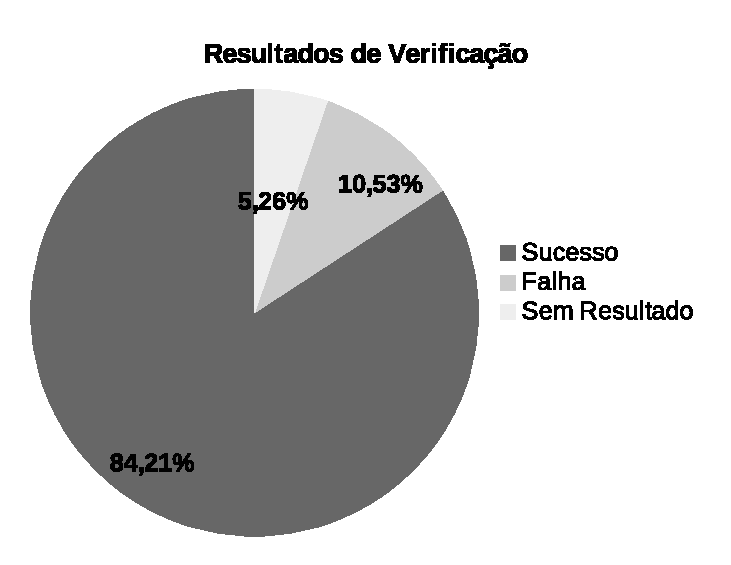
\includegraphics[scale=0.75]{figures/verification_results}
\caption{Resumo dos resultados de verifica��o}
\label{figure:summary-verification-results}
\end{figure*}

A Figura~\ref{figure:summary-verification-time} mostra um resumo do tempo de verifica��o necess�rio para cada benchmark. Treze programas levaram menos de $2$ segundos, de forma a avaliar as falhas existentes e as atribui��es associadas para produzir uma execu��o bem-sucedida, tr�s programas n�o foram verificados corretamente, com tempos associados de verifica��o menores que  $2$ segundos, e, finalmente, tr�s benchmarks levaram cerca de $4$ a $5$ vezes mais para produzir resultados �teis. Com rela��o ao �ltimo caso, analizando o processo de verifica��o do verificador de modelos, foi poss�vel apontar o gargalo como sendo o solucionador SMT, devido � quantidade de fontes de n�o-determinismo presentes em tais benchmarks. No entanto, o tempo de verifica��o em m�dia ainda � baixo, se comparado com o que pode ser obtido com depura��o de programas n�o-assistida~\cite{Mayer:2008}.

\begin{figure*}[htb]
\centering
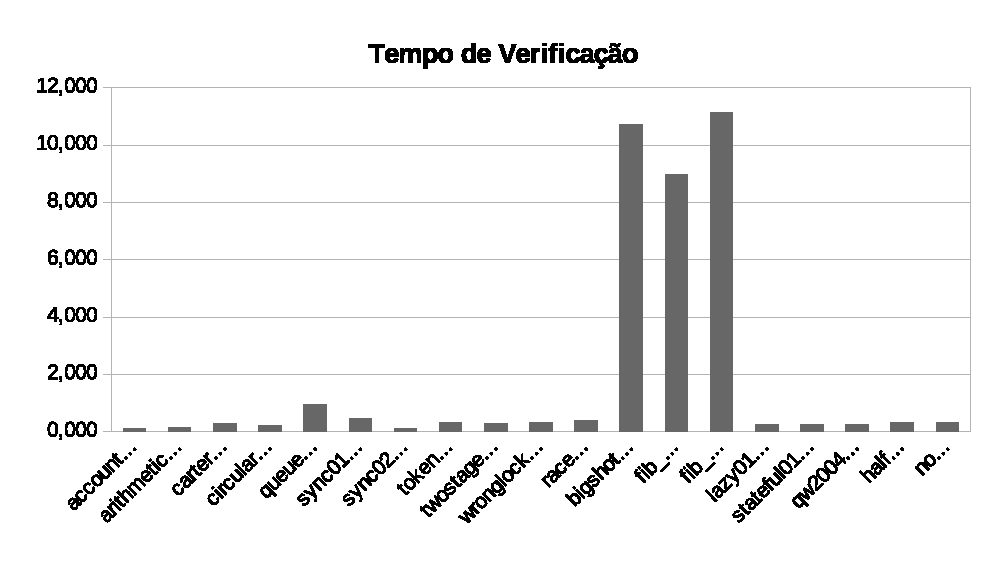
\includegraphics[scale=0.75]{figures/verification_time}
\caption{Resumo dos resultados de todos os benchmarks}
\label{figure:summary-verification-time}
\end{figure*}

Em resumo, os resultados apresentados mostram que a metodologia proposta � apropriada para localizar falhas em programas concorrentes em C, e que o tempo de verifica��o necess�rio para produzir uma execu��o bem-sucedida do programa � curto. Logo, a metodologia proposta pode ser �til para auxiliar desenvolvedores a depurar programas.

\section{Resumo}\label{chap-5-summary}

Neste cap�tulo apresentou a avalia��o experimental realizada para o m�todo proposto neste trabalho, assim como considera��es a serem feitas sobre a metodologia apresentada. O experimento foi conduzido com um computador padr�o e os dados obtidos foram analizados, mostrando a viabilidade do m�todo para encontrar linhas defeituosas em c�digos concorrentes, tendo uma taxa de sucesso de $84$.$21$\%, considerando todos os benchmarks propostos. A metodologia proposta mostrou-se �til para determinar as linhas defeituosas em um programa concorrente. No entanto, a depend�ncia de um contraexemplo para iniciar o processo de transforma��o de c�digo levou a alguns benchmarks n�o serem avaliados, pois o ESBMC n�o foi capaz de retornar um contraexemplo para os mesmos. Tamb�m � importante notar que ap�s a transforma��o de c�digo ser feita, o tempo de verifica��o do c�digo instrumentado foi sempre menor que $1$ segundo. De modo geral, a metodologia garante que a corre��o no c�digo original das linhas obtidas nos contraexemplos do novo c�digo sequencial levam a uma execu��o bem-sucedida do programa.

\chapter{Conclus�es}\label{chap_conclusion}

\section{Considera��es Finais}

Nesta disserta��o foi apresentado um m�todo para localizar falhas em programas concorrentes em C, usando regras de sequencializa��o e t�cnicas de verifica��o de modelos limitada. Este trabalho consistiu na transforma��o linha a linha do c�digo original concorrente com o intuito de simular o mesmo comportamento presente no �ltimo, e ent�o aplicar o m�teodo proposto por Griesmayer {\it et al.}~\cite{Griesmayer:2007} para obter as linhas que levam a uma viola��o de uma dada propriedade do programa, representando linhas existentes no programa concorrente.

Com rela��o aos resultados experimentais, a metodologia proposta foi capaz de identificar potenciais falhas em software concorrente, em $84$.$21$\% dos benchmarks escolhidos, enquanto falhou em obter linhas defeituosas �teis em tr�s dos benchmarks adotados. De fato, um deles apresentou um bloqueio fatal e os outros dois falham devido a problemas de sincroniza��o de \textit{threads}, o que necessita de uma investiga��o mais a fundo, de forma a prover aprimoramentos relacionados �s abordagens de modelagem das primitivas de sincroniza��o do C. No entanto, o m�todo � �til para avaliar programas concorrentes que apresentam falhas relacionadas a assertivas mal-formuladas e bloqueios fatais, o que o torna interessante para auxiliar desenvolvedores a encontrar atribui��es que levem a execu��es bem-sucedidas de programas e, consequentemente, minimiza o esfor�o em depura��o de c�digo.

Ao ser comparado com outras abordagens, o m�todo proposto � capaz de localizar falhas em programas concorrentes usando apenas o c�digo-fonte do programa, ao inv�s de um caminho mal-sucedido e uma su�te de teste. Ele tamb�m � capaz de n�o somente apontar as linhas defeituosas, como tamb�m prover poss�veis consertos para produzir execu��es bem-sucedidas do programa.

Durante o desenvolvimento deste trabalho foram identificados pontos que diminuem a efici�ncia do m�todo proposto. Dentre esses pontos, tamb�m observados na avalia��o experimental, pode-se destacar a necessidade de um contraexemplo para a posterior aplica��o do m�todo, dependendo inteiramente da capacidade do verificador de modelos de encontrar viola��es no programa original. Este problema est� relacionado diretamente � tarefa de custo mais elevado no m�todo proposto, que � a defini��o do vetor \texttt{cs}. Uma defini��o arbrit�ria, por meio de uso de t�cnicas de BMC, pode ser estudado em trabalhos posteriores.

Outro ponto a se considerar � a modelagem de estruturas da biblioteca {\it pthread}. Internamente, o ESBMC implementa um modelo para as primitivas de sincroniza��o da biblioteca, e neste trabalho define-se uma modelagem em um n�vel anterior � tradu��o interna do ESBMC. Deve-se tamb�m investigar qual das duas modelagens deve ser adotada com o objetivo de melhorar os resultados obtidos.

Apesar dos pontos descritos anteriormente, quando se trata do m�todo proposto para localizar falhas, o tempo de verifica��o � curto (geralmente menor que $1$ segundo) para o programa sequencial instrumentado n�o-determin�stico, possibilitando um diagn�stico r�pido para o mesmo.

De maneira geral, pode-se concluir que os objetivos espec�ficos desta disserta��o tamb�m foram atingidos.

Em uma empresa de desenvolvimento de software � comum o uso de programa��o concorrente para prover solu��es com tempo menor de resposta. Por�m, esta classe de programas est� sujeita a erros mais dif�ceis de serem corrigidos, e por consequ�ncia, erros que levem mais tempo para serem encontrados. O uso de um m�todo para localizar falhas em tais programas reduziria drasticamente o tempo associado a esta tarefa, melhorando o processo de desenvolvimento de software concorrente. O m�todo proposto nesta disserta��o visa ser uma alternativa para depura��o comum, usando uma t�cnica tamb�m em ascens�o para busca por defeitos, a verifica��o de modelos.

\section{Propostas para Trabalhos Futuros}

Nesta se��o ser�o apresentadas algumas propostas para desenvolvimentos futuros relacionados ao m�todo proposto descrito nesta disserta��o. Estas propostas podem ser dividas em duas categorias. Na primeira, � considerado o problema de sequencializa��o e modelagem de c�digo, e, na segunda, ser�o apresentadas propostas que visam melhorar a aplicabilidade do m�todo em geral.

Quanto ao problema de sequencializa��o e modelagem de c�digo:

\begin{itemize}

\item Novas regras para transforma��o devem ser adicionadas para que seja poss�vel representar melhor o programa original em rela��o �s intercala��es entre as {\it threads} existentes.

\item Melhorias na gram�tica para que seja poss�vel diagnosticar melhor problemas relacionados a declara��es relacionadas � biblioteca {\it pthread}.

\item O uso de desdobramento de la�os para melhor representa��o de la�os existentes em programas concorrentes, onde tamb�m podem existir trocas de contexto.

\end{itemize}

Quanto ao problema de aplicabilidade do m�todo em geral:

\begin{itemize}

\item Um {\it plugin} deve ser desenvolvido em um ambiente de desenvolvimento, como o {\it Eclipse}, de forma a automatizar o processo de localiza��o de falhas.

\item Propor uma estrat�gia para simular todas as intercala��es poss�veis, retirando o processo de defini��o do escalonamento definido em c�digo do verificador de modelos.

\item Incorporar a abordagem proposta por Gadelha {\it et al.}~\cite{Nicole:2017} para minimizar o esfor�o necess�rio para encontrar um contraexemplo para um programa concorrente defeituoso.

\item Aplicar o m�todo em outros seguimentos de programas, {\it e.g.}, programas concorrentes em Qt~\cite{Monteiro:2017}.

\end{itemize}


\bibliographystyle{abntex2-num}
\bibliography{references/references}

\appendix

\chapter{Publica��es}

\section{Referente � Pesquisa}

%\begin{itemize}

%\item \textbf{Alves, E. H. S.}, Cordeiro, L. C., Lima Filho, E. B. {\it Fault Localization in Multi-Threaded C Programs using Bounded Model Checking}. Em V Simp�sio Brasileiro de Engenharia de Sistemas Computacionais (SBESC), 2015. (\textbf{Publicado})~\cite{AlvesCF15}
%
%\item \textbf{Alves, E. H. S.}, Cordeiro, L. C., Lima Filho, E. B. {\it A Method to Localize Faults in Concurrent C Programs}. Em \textit{Journal of Software and Systems}, 2017. (\textbf{Publicado})~\cite{AlvesCF17}

%\end{itemize}

\section{Contribui��es em outras Pesquisas}

\begin{itemize}
\item \textbf{Cavalcante, T. R. F.}, Alves, E. H. S., Carvalho, C. B. \textit{Radio Communication to Control and Run an Autonomous Mission for UAVs via a Mobile Application}. Em IV Escola Regional de Inform�tica (ERIN), 2017. (\textbf{Publicado})
\item \textbf{Cavalcante, T. R. F.}, de Bessa, I. V., Cordeiro, L. C. \textit{Planning and Evaluation of UAV Mission Planner for Intralogistics Problems}. Em VII Simp�sio Brasileiro de Engenharia de Sistemas Computacionais (SBESC), 2017. (pp. 9-16). IEEE. (\textbf{Publicado})~\cite{cavalcante2017planning}
\end{itemize}

\chapter{\textit{Benchmarks} Utilizados}\label{appendix:bench}

\begin{table}[ht]
\centering
\caption{Descri��o dos \textit{benchmarks} usados nos experimentos do trabalho.}
\label{table:bench}
\footnotesize
\resizebox{0.9\textwidth}{!}{%
\begin{tabular}{|c|c|c|c|c|c|}
\hline
\textbf{ID} & \textbf{$A$} & \textbf{$B$} & \textbf{$C$} & \textbf{$t_{\mathrm{sr}}$ (s)} & \textbf{$PO_{\mathrm{r}}$} \\ \hline
1           & $ \begin{bmatrix}
-0.5 & 1.0 \\
0.0 & -0.5 
\end{bmatrix}  $ & $ \begin{bmatrix}
0.0 \\
2.5 
\end{bmatrix} $                                                              & $ \begin{bmatrix}
0.0 & 2.6 
\end{bmatrix} $                                                                                                                        & 2.5 & 5              \\
2           & $ \begin{bmatrix}
-0.5 & 1.0 & 0.0 \\
0.0 & -0.5 & 1.0 \\
0.0 & 0.0 & -0.5 
\end{bmatrix}  $ & $ \begin{bmatrix}
-0.4 \\
2.5 \\
-0.8 
\end{bmatrix} $ & $ \begin{bmatrix}
0.0 & 2.6 & 0.0 
\end{bmatrix} $ & 3.5     & 5          \\
3           & $ \begin{bmatrix}
-0.5 & 1.0 & 0.0 & 0.0 \\
0.0 & -0.5 & 1.0 & 0.0 \\
0.0 & 0.0 & -0.5 & 1.0 \\
0.0 & 0.0 & 0.0 & -0.5 
\end{bmatrix}  $ & $ \begin{bmatrix}
1.0 \\
2.5 \\
1.0 \\
1.0 
\end{bmatrix} $ & $ \begin{bmatrix}
0.0 & 2.6 & 1.2 & 0.0 \end{bmatrix} $ & 4.5      & 30         \\
4           & $ \begin{bmatrix}
-0.5 & 1.0 & 0.0 & 0.0 & 0.0 \\
0.0 & -0.5 & 1.0 & 0.0 & 0.0 \\
0.0 & 0.0 & -0.5 & 1.0 & 0.0 \\
0.0 & 0.0 & 0.0 & -0.5 & 1.0 \\
0.0 & 0.0 & 0.0 & 0.0 & -0.5 
\end{bmatrix}  $ & $ \begin{bmatrix}
-0.4 \\
-0.6 \\
5.5 \\
1.0 \\
-0.3 
\end{bmatrix} $ & $ \begin{bmatrix}
0.0 & 2.6 & 0.5 & 1.2 & 0.0 \end{bmatrix} $ & 5.5          & 20     \\
5           & $ \begin{bmatrix}
-0.5 & 0.4 \\
-0.4 & -0.5 
\end{bmatrix}  $                                                                                                                                           & $ \begin{bmatrix}
0.0 \\
2.5 
\end{bmatrix} $                                                                                                                           & $ \begin{bmatrix}
0.0 & 2.6 \end{bmatrix} $                                                                                                                        & 3.0    & 5           \\
6           & $ \begin{bmatrix}
-0.5 & 0.4 & 1.0 & 0.0 \\
-0.4 & -0.5 & 0.0 & 1.0 \\
0.0 & 0.0 & -0.5 & 0.4 \\
0.0 & 0.0 & -0.4 & -0.5 
\end{bmatrix}  $ & $ \begin{bmatrix}
0.0 \\
0.0 \\
2.5 \\
1.6 
\end{bmatrix} $ & $ \begin{bmatrix}
0.0 & 2.6 & 0.0 & 2.0 \end{bmatrix} $ & 5.0    & 30           \\
7           & $ \begin{bmatrix}
-0.5 & 0.4 & 0.0 & 0.0 \\
-0.4 & -0.5 & 0.0 & 0.0 \\
0.0 & 0.0 & -0.8 & 0.4 \\
0.0 & 0.0 & -0.4 & -0.8 
\end{bmatrix}  $ & $ \begin{bmatrix}
-0.4 \\
-0.6 \\
2.5 \\
1.6 
\end{bmatrix} $ & $ \begin{bmatrix}
0.0 & 2.6 & 0.0 & 2.0 \end{bmatrix} $ & 10.0          & 4    \\
8           & $ \begin{bmatrix}
-0.2 & 0.0 \\
0.0 & -0.3 
\end{bmatrix}  $                                                                                                                                            &$ \begin{bmatrix}
-0.6 \\
2.5 
\end{bmatrix} $                                                                                                                          & $ \begin{bmatrix}
0.0 & 2.6 
\end{bmatrix} $                                                                                                                        & 1.5         & 8      \\
9           & $ \begin{bmatrix}
-0.2 & 0.0 & 0.0 \\
0.0 & -0.3 & 0.0 \\
0.0 & 0.0 & -0.7 
\end{bmatrix}  $ & $ \begin{bmatrix}
-0.8 \\
-0.7 \\
-0.5 
\end{bmatrix} $ & $ \begin{bmatrix}
0.0 & 2.6 & 0.0 \end{bmatrix} $ & 2.0       & 8        \\
10          & $ \begin{bmatrix}
-0.2 & 0.0 & 0.0 & 0.0 \\
0.0 & -0.3 & 0.0 & 0.0 \\
0.0 & 0.0 & -0.7 & 0.0 \\
0.0 & 0.0 & 0.0 & -0.9 
\end{bmatrix}  $ & $ \begin{bmatrix}
-0.4 \\
2.5 \\
1.0 \\
-0.7
\end{bmatrix} $ & $ \begin{bmatrix}
0.0 & 2.6 & 1.2 & 0.0 \end{bmatrix} $ & 5.0       & 30        \\
11          & $ \begin{bmatrix}
-0.2 & 0.0 & 0.0 & 0.0 & 0.0 \\
0.0 & -0.3 & 0.0 & 0.0 & 0.0 \\
0.0 & 0.0 & -0.7 & 0.0 & 0.0 \\
0.0 & 0.0 & 0.0 & -0.9 & 0.0 \\
0.0 & 0.0 & 0.0 & 0.0 & -0.5 
\end{bmatrix}  $ & $ \begin{bmatrix}
-0.5 \\
-0.2 \\
2.5 \\
2.0 \\
-0.8
\end{bmatrix} $ & $ \begin{bmatrix}
0.0 & 2.6 & 0.5 & 1.2 & 0.0 \end{bmatrix} $ & 10.0    & 18          \\
12          & $ \begin{bmatrix}
4.5 & 1.0 \\
0.0 & 4.5 
\end{bmatrix}  $ & $ \begin{bmatrix}
0.0 \\
2.5 
\end{bmatrix} $                                                                                                                           & $ \begin{bmatrix}
0.0 & 2.6 
\end{bmatrix} $                                                                                                                        & 8.0         & 10      \\
13          & $ \begin{bmatrix}
1.5 & 1.0 & 0.0 \\
0.0 & 1.5 & 1.0 \\
0.0 & 0.0 & 1.5 
\end{bmatrix}  $ & $ \begin{bmatrix}
-0.4 \\
2.5 \\
-0.8
\end{bmatrix} $ & $ \begin{bmatrix}
0.0 & 2.6 & 0.0 \end{bmatrix} $ & 10.0 & 9
\\
14          & $ \begin{bmatrix}
-0.5 & 0.4 & 0.0 & 0.0 \\
-0.4 & -0.5 & 0.0 & 0.0 \\
0.0 & 0.0 & -0.8 & 0.4 \\
0.0 & 0.0 & -0.4 & -0.8 
\end{bmatrix}  $ & $ \begin{bmatrix}
-0.4 \\
-0.6 \\
-0.4 \\
-0.6
\end{bmatrix} $ & $ \begin{bmatrix}
0.0 & 2.6 & 0.0 & 2.0 \end{bmatrix} $ & 10.0     & 2          
\\
15          & $ \begin{bmatrix}
-0.6386 & 0.4151 \\
-0.0098 & 0.8266
\end{bmatrix}  $ & $ \begin{bmatrix}
0.2442 \\
1.0745 
\end{bmatrix} $ & $ \begin{bmatrix}
0.1807 & 0.2076 
\end{bmatrix} $ & 6.5      & 5         \\
16          & $ \begin{bmatrix}
-1.0003 & -0.0002 & 0.0 \\
-8.0007 & -1.0003 & 0.0001 \\
0.0 & 0.0 & -0.9216 
\end{bmatrix}  $ & $ \begin{bmatrix}
0.0008 \\
0.0016 \\
1.9608 
\end{bmatrix} $ & $ \begin{bmatrix}
-0.00016 & -0.0000831 & 0.000016 
\end{bmatrix} $ & 10.5  & 8             \\
17          & $\mathcal{A}$ & $\mathcal{B}$ & $\mathcal{C}$ & 27.0  & 1                                
\\ \hline
\multicolumn{6}{|l|}{\textit{Veja as matrizes $\mathcal{A}$, $\mathcal{B}$ e $\mathcal{C}$ em} \texttt{https://goo.gl/fSwVVb}}
%\multicolumn{14}{l}{\textit{See matrices $\mathcal{A}$, $\mathcal{B}$, $\mathcal{C}$ and $\mathcal{K}$ at} \texttt{http://dsverifier.org}}                                                                                                                                                                                                                                                                                                                                                                                                                                                                                                                                         \\ 
\\ \hline
\end{tabular}}
\end{table}

\end{document}

